\chapter{Equilibrio Estelar Relativista}\label{cap:Eq-Rel}

\section{M'etrica de Schwarzschild interna}

\subsection{Ecuaciones de Einstein para un fluido ideal}\label{sec:einsteinfluido}
En el presente cap'itulo, se estudiar'a una soluci'on para las ecuaciones de campo de Einstein \eqref{EE1} dentro de una estrella esf'erica y est'atica en equilibrio hidrost'atico, extendiendo el an'alisis del cap'itulo anterior para incluir los efectos de Relatividad General. Esto complementa la soluci'on en el vac'io de Schwarzschild encontrada en la secci'on \eqref{solucion_sch}, pues a diferencia de ella, que describe el campo gravitacional \emph{fuera} de una masa esf'erica y sim'etrica, ahora podremos describir el espacio-tiempo \emph{dentro} de dicha distribuci'on de materia, a trav'es de la \emph{m'etrica de Schwarzschild interna}.

\subsubsection{Tensor energ'ia-momentum de un fluido ideal}
Para encontrar la soluci'on interna se supondr'a, al igual que en el caso de Schwarzschild, que la m'etrica para un espaciotiempo esf'erico y est'atico est'a dada por \eqref{dsoriginal}, pero sin la dependencia temporal. Adem'as, se modelar'a la materia dentro de la estrella como un fluido ideal. De este modo, el lado derecho de las ecuaciones de campo \eqref{EE1} estar'a descrito por la distribuci'on de energ'ia dentro de la estrella, dada a trav'es del tensor de energ'ia-momentum de un fluido ideal:
\begin{equation}\label{tem}\marginnote{Tensor de energ'ia-momentum de un fluido ideal}
T_{\mu\nu}=\left(\rho+\dfrac{P}{c^2}\right)u_{\mu}u_{\nu}-Pg_{\mu\nu}.
\end{equation}
 La principal diferencia entre (\ref{tem}) y \eqref{temfp} es la generalizaci'on de la m'etrica de Minkowski $\eta_{\mu\nu}$, usada en Relatividad Especial, a la m'etrica general del espacio-tiempo $g_{\mu\nu}$, usada en Relatividad General. Adicionalmente, consideramos que la presi'on y densidad propia de masa dependen s'olo de la coordenada $r$, es decir, $P=P(r)$ y $\rho=\rho(r)$, ya que
la distribuci'on es esf'ericamente sim'etrica y est'atica.

Ahora bien, como estamos considerando el caso est'atico, las componentes espaciales de la cuadrivelocidad de cada elemento del fluido, en coordenadas de curvatura, se anulan:
\begin{equation}\label{uu}
 u^{\mu}(x)=\frac{dx^{\mu}}{d\tau}=(u^0,0,0,0).
\end{equation}
Dado que el elemento de l'inea se escribe en funci'on de la m'etrica de acuerdo a \eqref{dsymet}, es posible obtener la siguiente identidad para la cuadrivelocidad:
% \begin{equation}\label{dsymet}
%  ds^2=g_{\mu\nu}dx^{\mu}dx^{\nu},
% \end{equation}
\begin{equation}\label{cuadri}
g_{\mu\nu}u^{\mu}u^{\nu}\equiv c^2=g_{00}(u^0)^2\quad\Rightarrow\quad u^{0}=c\exp^{-\frac{1}{2}\alpha(r)}.
\end{equation}
Bajando el 'indice con la m'etrica \eqref{dsoriginal}, obtenemos
\begin{equation}\label{u0}
 u_0=g_{0\mu}u^{\mu}=g_{00}u^{0}=c\,e^{\frac{1}{2}\alpha(r)}.
\end{equation}
Por lo tanto, reemplazando la m'etrica y las componentes de la cuadrivelocidad  \eqref{uu} y \eqref{u0} en el tensor energ'ia-momentum (\ref{tem}), tenemos que s'olo sus cuatro elementos diagonales ser'an no nulos:
\begin{align}
T_{00}&=\rho c^2 e^{\alpha},\nonumber\\
T_{11}&=P e^{\beta},\nonumber\\
T_{22}&=P r^2,\label{tem2}\\
T_{33}&=T_{22}\sen^2\theta=P r^2\sen^2\theta,\nonumber
\end{align}
es decir,
\marginnote{Tensor de energ'ia-momentum de un fluido ideal est'atico}\begin{equation}\label{tem3}
 \boxed{T_{\mu\nu}=diag(\rho c^2 e^{\alpha},P e^{\beta},P r^2,P r^2\sen^2\theta).}
\end{equation}
De aqu'i se observa que la cuarta componente s'olo difiere en un factor de la tercera, $T_{33}=T_{22}\sen^2\theta$. Adem'as, tomando la traza de (\ref{tem}), usando (\ref{cuadri}), y la definici'on de m'etrica inversa, tenemos que
\begin{align}\label{traza}
T:=T^{\mu}_{\mu}=T_{\mu\nu}g^{\mu\nu}&=\left(\rho+\dfrac{P}{c^2}\right)u_{\mu}u_{\nu}g^{\mu\nu}-Pg_{\mu\nu}g^{\mu\nu}\\
&=\left(\rho+\dfrac{P}{c^2}\right)c^2-P\delta_{\mu}^{\mu}\\
&=\rho c^2-3P.
\end{align}

\subsubsection{Ecuaciones a resolver y procedimiento}
Tenemos todos los elementos necesarios para determinar el lado derecho de las ecuaciones de campo (\ref{EE1}). Reemplazando el tensor energ'ia-momentum de las ecs. (\ref{tem2}), su traza de (\ref{traza}), y la m'etrica de \eqref{dsoriginal}, notamos primero que $R_{\mu\nu}=0,\;\forall\; \mu\neq\nu$. Luego, las ecuaciones no nulas ser'an las componentes diagonales:

\begin{align}
 R_{00}&=\frac{8\pi G}{c^{4}}\left( T_{00}-\dfrac{1}{2}g_{00}T\right)=
% \frac{8\pi G}{c^{4}}\left( \rho c^2e^{\alpha}-\dfrac{1}{2}e^{\alpha}(\rho c^2-3P)\right)=
\frac{4\pi G}{c^{4}}(\rho c^2+3P)e^{\alpha},\\
R_{11}&=\frac{8\pi G}{c^{4}}\left( T_{11}-\dfrac{1}{2}g_{11}T\right)=
% \frac{8\pi G}{c^{4}}\left(Pe^{\beta}-\dfrac{1}{2}(-e^{\beta})(\rho c^2-3P)\right)=
\frac{4\pi G}{c^{4}}(\rho c^2-P)e^{\beta},\\
R_{22}&=\frac{8\pi G}{c^{4}}\left(T_{22}-\dfrac{1}{2}g_{22}T\right)=
% \frac{8\pi G}{c^{4}}\left(Pr^2-\dfrac{1}{2}(-r^2)(\rho c^2-3P)\right)=
\frac{4\pi G}{c^{4}}(\rho c^2-P)r^2\\
R_{33}&=R_{22}\sen^2\theta.
\end{align}

Ahora, el lado izquierdo de las ecuaciones anteriores se calcula a partir a partir de las componenes de la m'etrica \eqref{dsoriginal}. Esto ya se hizo en las ecuaciones \eqref{ricci00}-\eqref{ricci33}, por lo que aplic'andolas al caso est'atico aqu'i considerado, todas las derivadas temporales se anulan. Entonces, tendremos 3 ecuaciones de campo relevantes (ya que $R_{33}$ s'olo difiere en un factor $\sen^2\theta$ de $R_{22})$:
\begin{align}
R_{00}&=\frac{1}{2}e^{\alpha-\beta}\left[\alpha''-\frac{\beta'\alpha'}{2}+\frac{2\alpha'}{r}+\frac{\alpha'^2}{2}\right]=\frac{4\pi G}{c^{4}}\left( \rho c^2+3P\right)e^{\alpha},\label{ricci0}\\
R_{11}&=-\frac{1}{2}\left[\alpha''-\frac{\beta'\alpha'}{2}-\frac{2\beta'}{r}+\frac{\alpha'^2}{2}\right]=\frac{4\pi G}{c^{4}}\left( \rho c^2-P\right)e^{\beta},\label{ricci1} \\
R_{22}&=1-e^{-\beta}\left[1-\frac{1}{2}r\beta'+\frac{1}{2}r\alpha'\right]=\frac{4\pi G}{c^{4}}\left( \rho c^2-P\right)r^2. \label{ricci2}
\end{align}

\subsubsection{Obtenci'on del coeficiente m'etrico \texorpdfstring{$\beta$}{B}}
Ahora resolveremos el sistema de ecuaciones anterior. Primero despejaremos el coeficiente de la m'etrica $\beta(r)$ realizando la siguiente operaci'on sobre los coeficientes m'etricos:
\begin{align}
 &\frac{1}{2}e^{-\alpha}R_{00}+\frac{1}{2}e^{-\beta}R_{11}+r^{-2}R_{22}=e^{-\beta}\left(\frac{\beta'}{r}-\frac{1}{r^2}\right)+\frac{1}{r^2}=\frac{8\pi G}{c^2}\rho.
\end{align}

La relaci'on anterior implica, multiplic'andola por $r^2$, para despu'es integrar de $r'=0$ a $r'=r$, que
\begin{gather}
e^{-\beta}\beta' r-e^{-\beta}+1=\frac{8\pi G}{c^2}\rho r^2,\\
 \frac{d}{dr}\left( e^{-\beta}r\right) =1-\frac{8\pi G}{c^2}\rho r^2,\\
 \int\limits_{0}^r\frac{d}{dr'}\left( e^{-\beta(r')}r'\right)\,dr' =\int\limits_{0}^r \left(1-\frac{8\pi G}{c^2}\rho(r') r'^2\right)\,dr',\\
 r\,e^{-\beta(r)}-\lim_{r\to0}r\,e^{-\beta(r)}=r-\int\limits_{0}^r \frac{8\pi G}{c^2}\rho(r') r'^2\,dr',\\
e^{-\beta(r)}=1+\frac{1}{r}\lim_{r\to0}r\,e^{-\beta(r)}-\frac{1}{r}\int\limits_{0}^r \frac{8\pi G}{c^2}\rho(r') r'^2\,dr',\\
e^{\beta(r)}=\left(1+\frac{1}{r}\lim_{r\to0}r\,e^{-\beta(r)}-\frac{2G\mathcal{M}(r)}{c^2r}\right)^{-1}.
\end{gather}
En el 'ultimo paso se ha usado la misma definici'on de la funci'on de masa $\mathcal{M}(r)$ que en caso newtoniano, es decir,  (\ref{masa1}).

Asumimos que el coeficiente m'etrico $g_{11}=-B=-e^{\beta}$ es \textit{no singular en} $r=0$, de modo que $\lim_{r\to0}r\,e^{-\beta(r)}=0$, y as'i, el segundo coeficiente m'etrico ser'a finalmente:
\begin{equation}\label{beta}
% \boxed{e^{\beta(r)}=-\ln\left(1-\frac{2G\mathcal{M}(r)}{c^2r}\right)}\qquad \text{'o}\qquad
\boxed{B(r)=e^{\beta(r)}=\dfrac{1}{1-\frac{2G\mathcal{M}(r)}{c^2r}}.}
\end{equation}

\subsubsection{Obtenci'on del coeficiente m'etrico \texorpdfstring{$\alpha'$}{'a}}
Para hallar el otro coeficiente m'etrico $\alpha(r)$, es 'util usar el hecho que la derivada covariante del tensor energ'ia-momentum es id'enticamente nula (ver \eqref{dcT0}):
\begin{equation}\label{cons}
 \nabla_{\nu}T^{\mu\nu}=\partial_{\nu}T^{\mu\nu}+\Gamma^{\nu}_{\nu\lambda}T^{\lambda\mu}+\Gamma^{\mu}_{\nu\lambda}T^{\lambda\nu}=0.
\end{equation}

La relaci'on anterior es la generalizaci'on a campos gravitacionales no nulos de la ley de conservaci'on de energ'ia y momentum de un sistema. Es consecuencia directa de las ecuaciones de campo \eqref{EE1} y representa la versi'on relativista de las ecuaciones de continuidad y de Euler para un fluido ideal. Para evaluar las ecuaciones contenidas en la relaci'on anterior, se necesitan los s'imbolos de Christoffel, que fueron determinados en \eqref{gammas1_sch}-\eqref{gammas3_sch}. Adem'as, se requiere el tensor de energ'ia-momentum con los dos 'indices contravariantes, subiendo los 'indices de \eqref{tem3}:
\begin{equation}
 T^{\mu\nu}=g^{\mu\lambda}g^{\nu\rho}T_{\lambda\rho}=diag\left(\rho c^2 e^{-\alpha},P e^{-\beta},\frac{P}{r^2}, \frac{P}{r^2\sen^2\theta}\right).
\end{equation}
Entonces, de los s'imbolos de Christoffel no nulos se pueden determinar los dos 'ultimos t'erminos del lado derecho de la ecuaci'on de conservaci'on (\ref{cons}):
\begin{align}
 \Gamma^{\nu}_{\nu\lambda}T^{\lambda\mu}&=\Gamma_{01}^{0}T^{1\mu}+\Gamma_{11}^{1}T^{1\mu}+\Gamma_{21}^{2}T^{1\mu}+\Gamma_{31}^3T^{1\mu}+\Gamma_{32}^3T^{2\mu}\\&=T^{1\mu}\left(\frac{\alpha'}{2}+\frac{\beta'}{2}+\frac{2}{r}\right)+T^{2\mu}(\cot\theta),\\
\Gamma^{\mu}_{\nu\lambda}T^{\lambda\nu}&=\Gamma_{00}^{\mu}T^{00}+\Gamma_{11}^{\mu}T^{11}+\Gamma_{22}^{\mu}T^{22}+\Gamma_{33}^{\mu}T^{33}\\&=\rho c^2e^{-\alpha}\Gamma^{\mu}_{00}+Pe^{-\beta}\Gamma^{\mu}_{11}+\frac{P}{r^2}\Gamma^{\mu}_{22}+\frac{P}{r^2\sen^2\theta}\Gamma^{\mu}_{33}.
\end{align}

Reemplazando lo anterior en (\ref{cons}), es posible evaluar la componente $\mu=1$:
\begin{align}
 0=\nabla_{\nu}T^{1\nu}&=\frac{\partial T^{11}}{\partial x^1}+\cancelto{0}{\frac{\partial T^{12}}{\partial x^2}}+\cancelto{0}{\frac{\partial T^{13}}{\partial x^3}}+\Gamma_{v\lambda}^{\nu}T^{\lambda1}+\Gamma_{\nu\lambda}^{1}T^{\lambda\nu}\\
&=\frac{\partial T^{11}}{\partial x^1}+\left\{T^{11}\left(\frac{\alpha'}{r}+\frac{\beta'}{2}+\frac{2}{r}\right)\right\} \nonumber\\
&\quad+\left\{\rho c^2 e^{-\alpha}\Gamma^{1}_{00}+Pe^{-\beta}\Gamma^{1}_{11}+\frac{P}{r^2}\Gamma^{1}_{22}+\frac{P}{r^2\sen^2\theta}\Gamma^{1}_{33}\right\}\\
&=\frac{\partial}{\partial r}(Pe^{-\beta})+Pe^{-\beta}\left(\frac{\alpha'}{r}+\frac{\beta'}{2}+\frac{2}{r}\right) \nonumber\\
&\quad+\rho c^2 e^{-\alpha}\left(\frac{1}{2}\alpha'\, e^{\alpha-\beta}\right)+Pe^{-\beta}\left(\frac{\beta'}{2}\right) \nonumber\\
&\phantom{+}+\frac{P}{r^2}(-re^{-\beta})+\frac{P}{r^2\sen^2\theta}(-r^2\sen^2\theta e^{-\beta})\\
&=e^{-\beta}\left[P'+\frac{P\alpha'}{2}+\frac{\rho c^2 \alpha'}{2}\right].
\end{align}

Por lo tanto, al despejar $\alpha'$ se obtiene\footnote{Es posible mostrar que esta expresi'on se reduce, en el caso no relativista, a la ecuaci'on de equilibrio hidrost'atico en un potencial gravitacional $\phi$. Ver la secci'on (\ref{sec:tov}) para m'as detalles.}:
\begin{equation}\label{alpha'}
 \alpha'=-2\frac{P'}{P+\rho c^2}=-2\frac{\,dP/dr}{P+\rho c^2}.
\end{equation}


\subsubsection{Obtenci'on de la ecuaci'on T.O.V. para \texorpdfstring{$P'$}{P}}
A continuaci'on, reemplazando la ecuaci'on \eqref{beta} para $\beta$, y la reci'en obtenida \eqref{alpha'} para $\alpha'$,  en la componente $R_{22}$ del tensor de Ricci, ec. (\ref{ricci2}), podemos notar que obtenemos una ecuaci'on sin ambos coeficientes m'etricos, pudiendo determinar as'i $P':=dP/dr:$

\begin{align}
 R_{22}&=\frac{4\pi G}{c^{4}}\left( \rho  c^2-P\right)r^2\\
&=1-e^{-\beta}\left[1-\frac{1}{2}r\beta'+\frac{1}{2}r\alpha'\right]\\
&=1-\underbrace{\left(1-\frac{2G\mathcal{M}}{c^2r}\right)}_{\text{ec. (\ref{beta})}}\left[1-\frac{1}{2}r\frac{d}{dr}\underbrace{\left\{-\ln\left(1-\frac{2G\mathcal{M}}{c^2r}\right)\right\}}_{\text{ec. (\ref{beta})}}+\frac{1}{2}r\underbrace{\left(\frac{-2P'}{P+\rho c^2}\right)}_{\text{ec. (\ref{alpha'})}}\right]\\
&=1-\left(1-\frac{2G\mathcal{M}}{c^2r}\right)\left[1+\frac{1}{2}r\left\{\frac{1}{1-\frac{2G\mathcal{M}}{c^2r}}\left(\frac{2G\mathcal{M}}{c^2r^2}-\frac{2G\mathcal{M}'}{c^2\,r}\right)\right\}-\frac{r}{P+\rho c^2}P'\right]\\
&=\frac{2G\mathcal{M}}{c^2r}-\frac{1}{2}r\left(\frac{2G\mathcal{M}}{c^2r^2}-\frac{2G}{c^2r}\underbrace{4\pi r^2\rho}_{\text{ec. } \eqref{masa2}}\right)+\left(1-\frac{2G\mathcal{M}}{c^2r}\right)\frac{r}{P+\rho c^2}P'.
\end{align}

De este modo, despejando $P'$, podemos escribir
\begin{align}
 \left(1-\frac{2G\mathcal{M}}{c^2r}\right)\frac{r}{P+\rho c^2}P'&=\frac{4\pi G}{c^{4}}\left( \cancel{\rho c^2}-P\right)r^2-\frac{G\mathcal{M}}{c^2 r}-\cancel{\frac{4\pi Gr^2\rho}{c^2}},\\
\left(1-\frac{2G\mathcal{M}}{c^2r}\right)\frac{P'}{1+\frac{P}{\rho c^2}}\frac{r}{\rho c^2}&=-\frac{G\mathcal{M}}{c^2}\left(4\pi \frac{P r^2}{c^2\mathcal{M}}+\frac{1}{r}\right),\\
\left(1-\frac{2G\mathcal{M}}{c^2r}\right)\frac{P'}{1+\frac{P}{\rho c^2}}&=-\frac{G\mathcal{M}\rho}{r^2}\left(1+\frac{4\pi r^3}{c^2 \mathcal{M}}P\right).
\end{align}

As'i, hemos hallado $P'$ en funci'on de tres campos escalares conocidos: la presi'on $P(r)$, la densidad propia de masa $\rho(r)$ y la cantidad (sin interpretaci'on de momento) $\mathcal{M}(r)$, llegando a la famosa \textit{ecuaci'on de Tolman-Oppenheimer-Volkoff} (TOV)\footnote{Esta expresi'on fue derivada por Oppenheimer y Volkoff en 1939 (ver \cite{Oppenheimer39enero}), en base a trabajos anteriores de R. Tolman de los a\~nos 1934 y 1939.}:
\begin{equation}\label{tov}\marginnote{Ecuaci'on de T.O.V.}
\boxed{\frac{dP}{dr}=-\frac{G\mathcal{M}(r)\rho(r)}{r^2}\left[ 1+\frac{P(r)}{\rho c^2}\right]\left[ 1+\frac{4\pi r^3P(r)}{\mathcal{M}(r)c^2}\right]\left[ 1-\frac{2G\mathcal{M}(r)}{c^2r}\right]^{-1} .}
\end{equation}

\subsubsection{Obtenci'on del coeficiente m'etrico \texorpdfstring{$\alpha$}{a}}
 Notemos ahora que podemos reemplazar la ecuaci'on \eqref{tov} en la expresi'on para $\alpha'$ \eqref{alpha'}, y as'i obtener la forma expl'icita del coeficiente $\alpha$, integrando desde $r'=r$ a $r'\to\infty$:
\begin{align}
 \alpha'&=-\frac{2}{\rho c^2}\frac{1}{1+\frac{P}{\rho c^2}}\frac{dP}{dr}\\
&=\frac{2}{\rho(r) c^2}\frac{1}{1+\frac{P(r)}{\rho(r) c^2}}\frac{G\mathcal{M}(r)\rho(r)}{r^2}\left[ 1+\frac{P(r)}{\rho c^2}\right]\left[ 1+\frac{4\pi r^3P(r)}{\mathcal{M}(r)c^2}\right]\left[ 1-\frac{2G\mathcal{M}(r)}{c^2r}\right]^{-1}\\
&=\frac{2}{c^2}\frac{G\mathcal{M}(r)}{r^2}\left[ \frac{\mathcal{M}(r)c^2+4\pi r^3P(r)}{\mathcal{M}(r)c^2}\right]\left[ 1-\frac{2G\mathcal{M}(r)}{c^2r}\right]^{-1}. \label{dPdr1}
\end{align}
Equivalentemente, \eqref{dPdr1} puede encontrarse considerando la combinaci'on $e^{-\alpha}R_{00}/2+e^{-\beta}R_{11}/2-R_{22}/r^2$ a partir de \eqref{ricci0}-\eqref{ricci2} y luego usando \eqref{beta}. Por lo tanto,
\begin{align}
\int\limits_r^{\infty}\alpha'(r')dr'&=\int\limits_r^{\infty}\frac{2G}{c^2r'^2}\left[ \mathcal{M}(r')+\frac{4\pi r'^3P(r')}{c^2}\right]\left[ 1-\frac{2G\mathcal{M}(r')}{c^2r'}\right]^{-1}dr'.
\end{align}
Imponiendo la condici'on de borde: $\lim_{r\to\infty}\alpha=0$, que es equivalente a $\lim_{r\to\infty}g_{00}=1$ (pues $g_{00}=A=e^{\alpha}$), es decir, suponer que la m'etrica tiende asint'oticamente a la m'etrica plana de Minkowski en el infinito, obtenemos finalmente\footnote{Note que esta condici'on no restringe la generalidad de la soluci'on, puesto que se puede implementar por medio de un simple reescalamiento de la coordenada temporal $t$, de modo tal que 'esta coincida con el tiempo propio medido por observadores est'aticos en el infinito.}:
\begin{equation}\label{alpha1}
\boxed{\alpha(r)=-\frac{2G}{c^2}\int\limits_r^{\infty}\frac{dr'}{r'^2}\left[ \mathcal{M}(r')+\frac{4\pi r'^3P(r')}{c^2}\right]\left[ 1-\frac{2G\mathcal{M}(r')}{c^2r'}\right]^{-1},}
\end{equation}
\begin{equation}\label{alpha2}
\boxed{A(r)=\exp{\left[-\frac{2G}{c^2}\int\limits_r^{\infty}\frac{dr'}{r'^2}\left[ \mathcal{M}(r')+\frac{4\pi r'^3P(r')}{c^2}\right]\left[ 1-\frac{2G\mathcal{M}(r')}{c^2r'}\right]^{-1}\right]}.}
\end{equation}

\subsection{M'etrica de Schwarzschild interior}

En resumen, a partir de las ecuaciones de Einstein \eqref{EE1} en un espacio tiempo esf'ericamente sim'etrico y est'atico, con un tensor de energ'ia-momentum correspondiente a un fluido ideal de presi'on $P(r)$ y densidad $\rho(r)$ distribuido en una regi'on $r<R$ (estrella), se han hallado los coeficientes de la m'etrica \eqref{dsoriginal} $\alpha$  y $\beta$ (dados por \eqref{alpha1} y \eqref{beta}, respectivamente) en el interior de una estrella compuesta de dicho fluido, que es lo que se conoce como \emph{m'etrica de Schwarzschild interior}, determinando la geometr'ia del espacio-tiempo.

N'otese que para poder determinar completamente la m'etrica, se requiere conocer previamente, $\forall \;r<R$, los tres campos escalares que describen la estructura de la estrella: $\rho(r)$, $P(r)$, $\mathcal{M}(r)$. Para ello, se debe resolver en primer lugar las ecuaciones de estructura estelar que las determina, lo que analizaremos en la siguiente secci'on.
%Asumiendo conocidas esas cantidades, a'un falta una condici'on inicial para $\alpha$. Esto es
%as'i debido a que tenemos dos ecuaciones que determinan los dos primeros coeficientes de la
%m'etrica: (\ref{beta}) y (\ref{alpha1}). La primera de ellas es una ecuaci'on algebraica, pero %la segunda es una ecuaci'on integral en $\alpha$, que es equivalente a tener una ecuaci'on %diferencial de primer orden (ver \ref{alpha'}), que requiere una condici'on inicial para %determinar una soluci'on un'ivoca.

\subsubsection{Schwarzschild interior y exterior}\label{sec:interiorexterior}
Un primer test de consistencia para los coeficientes m'etricos hallados, es la verificaci'on que la soluci'on (m'etrica) de Schwarzschild interior se reduce a la conocida soluci'on de Schwarzschild exterior (\ref{Sch}). Para ello, se debe notar que la distribuci'on de masa caracterizada por $\rho(r)$, $P(r)$ y $\mathcal{M}(r)$ est'a limitada a un cierto rango $r<R$ (con $R$ definida como el radio de la estrella, de la misma forma que en el caso newtoniano). En cambio, el exterior de la estrella $r>R$ estar'a caracterizado por
\begin{equation}\label{condicionesexterior}
 \rho(r)=0,\quad P(r)=0,\quad \mathcal{M}(r)=\mathcal{M}(R)=M,
\end{equation}
en donde $M$ ser'ia el an'alogo relativista de la masa total de la estrella.
%(ver secci'on \ref{sec:masagravitacional} para detalles sobre la interpretaci'on).
Luego, el primer coeficiente m'etrico $g_{00}$ queda determinado al imponer las condiciones (\ref{condicionesexterior}) en (\ref{alpha1}):
\begin{align}\label{Arext1}
A(r)=e^{\alpha(r)}&=\exp{\left[-\frac{2G}{c^2}\int\limits_r^{\infty}\frac{dr'}{r'^2}\frac{M}{1-\frac{2GM}{c^2r'}}\right]},\qquad r>R.
\end{align}
Mediante la sustituci'on
\begin{equation}
x=1-\frac{2GM}{c^2r}\quad\Rightarrow\quad dx=\frac{2GM}{c^2r^2}dr,
\end{equation}
y dado que $r\to\infty\quad\Rightarrow\quad x=1$, obtenemos:
\begin{align}
A(x)&=\exp\left[-\int\limits_{x}^{1}\frac{dx'}{x'}\right]=\exp\left[\ln x-\ln 1\right]=x.
\end{align}
Volviendo a la variable original $r$, encontramos:
\begin{align} \label{Arext2}
A(r) =e^{\alpha(r)}&= 1-\frac{2GM}{c^2r}\qquad
\text{$r>R$}.
\end{align}
De forma an'aloga, el segundo coeficiente m'etrico $g_{11}$ se determina al imponer (\ref{condicionesexterior}) en (\ref{beta}):
\begin{equation}
 B(r)=e^{\beta(r)}=\dfrac{1}{1-\dfrac{2GM}{c^2r}},\qquad
\text{$r>R$}.
\end{equation}
Por lo tanto, el elemento de l'inea de la m'etrica de Schwarzschild interior se reduce a:
\begin{equation}
 ds^2=\left(1-\dfrac{2GM}{c^2r}\right)c^2dt^2-\dfrac{dr^2}{\left(1-\dfrac{2GM}{c^2r}\right)}-r^2(d\theta^2+\sen^2\theta d\varphi^2),\qquad
\text{$r>R$}.
\end{equation}
Esta soluci'on es precisamente la soluci'on (m'etrica) de Schwarzschild en el vac'io (soluci'on exterior) \eqref{Sch}, verificando as'i que la cantidad $M:=\mathcal{M}(R)$ es la masa total de la estrella.

\section{Ecuaci'on de Tolman-Oppenheimer-Volkoff}

\subsection{Ecuaciones de Estructura Estelar}\label{ecs-estructura-estelar}
Mientras se resolv'ian las ecuaciones de Einstein para hallar la soluci'on de Schwarzschild exterior (antes de obtener la forma expl'icita de $\alpha$), se obtuvo la ecuaci'on (\ref{tov}), que determinaba el gradiente de presi'on en el interior de la estrella, en funci'on de la coordenada radial $r$ y los campos $\rho(r)$ y $\mathcal{M}(r)$. Esta ecuaci'on de Tolman-Oppenheimer-Volkoff es de importancia fundamental para determinar un modelo estelar an'alogo al caso newtoniano descrito en el cap'itulo \ref{chap:eq_newton}, pues representa una generalizaci'on de la ecuaci'on \eqref{eqnewton} de equilibrio hidrost'atico newtoniano en Relatividad General. En efecto, en el l'imite no relativista, $P/\rho c^2\ll1$ y $G\mathcal{M}/rc^2\ll1$, por lo que (\ref{tov}) se reduce a \eqref{eqnewton}, puesto que cada uno de los factores en par'entesis cuadrados se aproxima a 1.

Entonces, es posible determinar un modelo estelar siguiendo la analog'ia con el cap'itulo \ref{chap:eq_newton} (ver secci'on \ref{resolviendo}), a partir de las ecuaciones de equilibrio hidrost'atico de \emph{Tolman-Oppenheimer-Volkoff}(\ref{tov}), ecuaci'on de estado (\ref{estado}) y de masa (\ref{masa2}):
\begin{align}
\frac{dP}{dr}&=-\frac{G\mathcal{M}(r)\rho(r)}{r^2}\left[ 1+\frac{P(r)}{\rho c^2}\right]\left[ 1+\frac{4\pi r^3P(r)}{\mathcal{M}(r)c^2}\right]\left[ 1-\frac{2G\mathcal{M}(r)}{c^2r}\right]^{-1},\marginnote{Ecs. de estructura estelar} \\
\frac{d\mathcal{M}(r)}{dr}&=4\pi r^2\rho(r),\\
P(r)&=P(\rho(r)).
\end{align}
Notemos que estas ecuaciones presentan la siguiente estructura:
\begin{align}
 P'(r)&=P'(P(r),\rho(r),\mathcal{M}(r)),\\
\mathcal{M}'(r)&=\mathcal{M}(\rho(r)),\\
P(r)&=P(\rho(r)).
\end{align}
As'i, de forma muy similar a la presentada en el caso newtoniano de la secci'on \ref{resolviendo}, tenemos tres ecuaciones para los campos escalares que determinan la estructura de la estrella (y a partir de las cuales es posible determinar la m'etrica). De ellas, dos son ecuaciones diferenciales de primer orden, por lo cual se requerir'an dos condiciones iniciales, dadas por las mismas expresiones que en la secci'on \ref{resolviendo}, aunque la interpretaci'on de la primera de ellas (para $\mathcal{M}$) ser'a diferente ahora (ya no es la ``masa'' dentro del radio $r$ de la estrella, sino una magnitud que incluye tanto su masa-energ\'ia en reposo, como tambi\'en a la energ\'ia del campo gravitacional que produce). Y al igual que en el cap'itulo \ref{chap:eq_newton}, integraremos las tres ecuaciones simult'aneamente desde el centro de la estrella hasta el sitio en que la presi'on y la densidad se anulen, definiendo as'i el radio de la estrella.


\subsection{Propiedades de la ecuaci'on TOV}\label{sec:tov}

Una propiedad que comparte la ec. (\ref{tov}) con su an'alogo newtoniano (\ref{eqnewton}) es que tambi'en es mon'otonamente decreciente, pues la densidad tambi'en  es definida positiva en este caso. Sin embargo, el gradiente de presi'on en la ecuaci'on relativista es mayor que en la expresi'on newtoniana, pues el denominador es m'as peque\~no, $\left(1-{2G\mathcal{M}(r)}/{c^2r}\right)<1$, y cada factor en el numerador es m'as grande:  $\left(1+{P(r)}/{\rho c^2}\right)>1$ y $1+{4\pi r^3P(r)}/{\mathcal{M}(r)c^2}>1$. Entonces, conforme $r\to0$, la presi'on relativista crece m'as r'apido que la newtoniana. Y dado que esto contribuye a incrementar los t'erminos de la presi'on en el denominador, el gradiente de 'esta ser'a a'un m'as grande conforme se vaya acercando al centro de la estrella. Podemos decir entonces que \textbf{la teor'ia de Relatividad General requiere (para mantener el equilibrio) campos m'as intensos que en la teor'ia de Newton, en el interior de una estrella}.

Este hecho tambi'en puede deducirse a partir de una ecuaci'on derivada antes de llegar a la ecuaci'on TOV: la expresi'on para $\alpha'$ (\ref{alpha'}). Primero, notemos que dicha ecuaci'on se reduce a la expresi'on newtoniana de equilibrio hidrost'atico newtoniano en un potencial gravitacional $\phi$. En efecto, en el l'imite no relativista, $\rho c^2\gg P$. Luego, la ec. (\ref{alpha'}) se reduce a
\begin{equation}
 \alpha'=(\ln A)'=\frac{A'}{A}\approx-2\frac{dP/dr}{\rho c^2}.
\end{equation}
Por otra parte, en el l'imite newtoniano, ver la ec. \eqref{g00phi}, el primer coeficiente m'etrico es
\begin{equation}
g_{00}=A=e^{\alpha}\approx1+\frac{2\phi}{c^2}.
\end{equation}
De este modo, dado que $A'=(2/c^2)d\phi/dr$ , es posible comparar con la ecuaci'on anterior y obtener
\begin{align*}
\alpha'=\frac{A'}{A}\approx2 \frac{d\phi/dr}{c^2}\frac{1}{1+\frac{2\phi}{c^2}}&\approx-2\frac{dP/dr}{\rho c^2}.
\end{align*}
Pero $2\phi/c^2\ll 1$, y por lo tanto
\begin{align*}
\frac{dP}{dr}&\approx-\rho\frac{d\phi}{dr},
\end{align*}
que es la ecuaci'on de equilibrio hidrost'atica newtoniana (\ref{equir}).

Otro hecho digno de ser destacado es que la ecuaci'on \eqref{tov} predice que las mayores fuerzas gravitacionales presentes dentro de una estrella, cuando se modela con Relatividad General, tienen como consecuencias que, dadas ciertas condiciones, algunas enanas blancas y estrellas supermasivas colapsan gravitacionalmente en circunstancias que la teor'ia de gravitaci'on newtoniana predecir'ia equilibrio hidrost'atico estable. Una de estas condiciones de estabilidad proviene de la simple inspecci'on de la ecuaci'on de Tolman-Oppenheimer-Volkoff, pues como el gradiente de presi'on debe ser siempre finito, se debe tener necesariamente que el 'ultimo t'ermino debe ser definido positivo:
\begin{equation}\marginnote{Condici'on de estabilidad relativista}
 \boxed{\frac{2G\mathcal{M}(r)}{c^2r}<1.}
\end{equation}
Esta condici'on es intr'insecamente relativista y no est'a presente en la teor'ia de Newton. En la siguiente secci'on se resolver'an, para el caso particular m'as simple posible, las ecuaciones de estructura estelar y se encontrar'an otras condiciones de estabilidad.


\section{Soluci'on: Densidad constante}

\subsection{Obteniendo la presi'on  \texorpdfstring{$P(r)$}{P(r)} relativista}
Ahora, an'alogamente al caso newtoniano, determinaremos la soluci'on de las ecuaciones de estructura estelar relativista para una estrella con distribuci'on de masa homog'enea de la forma:
\begin{equation}\label{er1}
 \rho(r)=\begin{cases}
  \rho_{\rm c}=\text{cte.}, & r<R\\
  0, & r>R.
\end{cases}
\end{equation}
Esta ecuaci'on de estado es independiente de la presi'on, as'i que estamos considerando materia incompresible. Esto corresponde al l'imite $\gamma\rightarrow\infty$ en la ecuaci'on de estado politr'opica (\ref{estadopolitropica}). Reemplazando en la ecuaci'on de definici'on de $\mathcal{M}(r)$ (\ref{masa1}) obtenemos entonces:
\begin{equation}\label{er2}
\boxed{\mathcal{M}(r)=\begin{cases}
\frac{4\pi}{3}\rho_{\rm c}r^3=M\frac{r^3}{R^3}, &r<R,\\
\frac{4\pi}{3}\rho_{\rm c}R^3=M,  & r > R.
\end{cases}}
\end{equation}
Insertando (\ref{er1}) y (\ref{er2}) en la ecuaci'on de Tolman-Oppenheimer-Volkoff (\ref{tov}), dentro del rango $r\leq R$ obtenemos:
\begin{align}
 P'=-\frac{4\pi G}{c^4}r\left[P+\rho_{\rm c} c^2\right]\left[P+\frac{1}{3}\rho_{\rm c}c^2\right]\left[ 1-\frac{8\pi G\rho_{\rm c}}{3c^2}r^2\right]^{-1}
\end{align}
Luego,
\begin{equation}\label{densidadcte1}
\frac{P'}{(P+\rho_{\rm c}c^2)(P+\rho_{\rm c}c^2/3)}=-\frac{4\pi G}{c^{4}}r\left[ 1-\frac{8\pi G\rho_{\rm c}}{3c^2}r^2\right]^{-1}.
\end{equation}
Introduciendo el radio adimensional $x:=\sqrt{8\pi G\rho_{\rm c}/3c^2}\,r$ tendremos:
\begin{equation}
\frac{-2\rho_{\rm c}c^2dP}{(P+\rho_{\rm c}c^2)(3P+\rho_{\rm c}c^2)}=\frac{x\,dx}{1-x^2}.
\end{equation}
La integral indefinida de esta ecuaci'on resulta ser (por ejemplo, usando el m'etodo de fracciones parciales):
\begin{equation}\label{Prhoc}
\ln\left( \frac{P+\rho_{\rm c}c^2}{3P+\rho_{\rm c}c^2}\right)=-\frac{1}{2}\ln(1-x^2)+\text{cte.}=\ln\left[a\left(1-x^2\right)\right]^{-1/2}
\end{equation}
La constante de integraci'on $a$ que hemos introducido puede encontrarse al considerar que la presi'on se anula en la superficie de la estrella, es decir $P(R)=0$. Con esto, obtenemos:
\begin{equation}
a=\frac{1}{1-\frac{8\pi G}{3 c^2}\rho_{\rm c} R^2}.
\end{equation}
Entonces \eqref{Prhoc} se puede escribir como:
\begin{equation}
\frac{P(r)+\rho_{\rm c}c^2}{3P(r)+\rho_{\rm c}c^2}=\left[\frac{1-8\pi G\rho_{\rm c}R^2/3c^2}{1-8\pi G\rho_{\rm c}r^2/3c^2} \right]^{1/2}, \qquad r\leq R.
\end{equation}
Introduciendo el radio de Schwarzschild: $r_S=2GM/c^2=8\pi G\rho_{\rm c}R^3/3c^2$, y despejando $P(r)$, tenemos:
\begin{gather}
% P(r)+\rho_{\rm c} c^2=\left(\frac{1-r_s/R}{1-r_s r^2/R^3}\right)^{1/2}\left(3P(r)+\rho_{\rm c} c^2\right)\\
P(r)=\rho_{\rm c} c^2\frac{\sqrt{\frac{1-r_s/R}{1-r_s r^2/R^3}}-1}{1-3\sqrt{\frac{1-r_s/R}{1-r_s r^2/R^3}}}.
\end{gather}
Simplificando, obtenemos que la soluci'on exacta y expl'icita para la presi'on en funci'on de la coordenada radial $r$ es dada por:
\begin{equation}\label{presioncondensidadcte}
\boxed{P(r)=\rho_{\rm c}c^2\frac{\sqrt{1-\frac{r_Sr^2}{R^3}}-\sqrt{1-\frac{r_S}{R}}}{ 3 \sqrt{1-\frac{r_S}{R}}-\sqrt{1-\frac{r_Sr^2}{R^3}}}, \qquad r\leq R.}
\end{equation}

\subsubsection{L'imite newtoniano}
Podemos verificar que la expresi'on \eqref{presioncondensidadcte} se reduce a la presi'on calculada seg'un la teor'ia newtoniana, es decir a \eqref{presionnewton}. Para ello, notamos que de acuerdo a lo discutido en referencia a la ecuaci'on \eqref{cuo}, la aproximaci'on newtoniana se conseguir'a cuando el radio de Schwarzschild $r_S$ de la estrella sea mucho menor que su radio $R$, por lo que, expandiendo \eqref{presioncondensidadcte} a primer orden en $r_S/R$, obtenemos:
\begin{align}
 P(r)&=\rho_{\rm c} c^2\frac{\left(1-\frac{1}{2}\frac{r_S}{R}\left(\frac{r}{R}\right)^2+\mathcal{O}\left(\frac{r_S}{R}\right)^2\right)-\left(1-\frac{1}{2}\frac{r_S}{R}+\mathcal{O}\left(\frac{r_S}{R}\right)^2\right)}{3\left(1-\frac{1}{2}\frac{r_S}{R}+\mathcal{O}\left(\frac{r_S}{R}\right)^2\right)-\left(1-\frac{1}{2}\frac{r_S}{R}\left(\frac{r}{R}\right)^2+\mathcal{O}\left(\frac{r_S}{R}\right)^2\right)}\\
&\approx\rho_{\rm c} c^2\frac{\frac{1}{2}\frac{r_S}{R}\left(\frac{-r^2+R^2}{R^2}\right)}{2\left[1+\frac{1}{4}\frac{r_S}{R}\frac{(-3R^2+r^2)}{R^2}\right]}\\
&=\rho_{\rm c} c^2\frac{1}{4}\frac{r_S}{R}\left(\frac{R^2-r^2}{R^2}\right)\left[1-\frac{1}{4}\frac{r_S}{R}\frac{(r^2-3R^2)}{R^2}\right]\\
&\approx\rho_{\rm c} c^2\frac{r_S}{4R^3}\left(R^2-r^2\right),
\end{align}
que coincide con la expresi'on newtoniana \eqref{presionnewton} para $P(r)$.

\subsection{Obteniendo los coeficientes m'etricos}
Resumiendo, hemos hallado las tres variables de estructura de la estrella: la densidad \eqref{er1}, la funci'on de masa \eqref{er2} y la presi'on en \eqref{presioncondensidadcte}. A continuaci'on, para determinar el coeficiente m'etrico $\alpha$ se recurre a \eqref{alpha1}. En este caso, debemos separar la integral en dos contribuciones, una interior ($r<r'<R$) y otra exterior $R<r'<\infty$. Entonces,
\begin{equation}
\alpha(r)=-\frac{2G}{c^2}\int\limits_r^R\frac{dr'}{r'^2}\frac{\left[ \mathcal{M}(r')+\frac{4\pi r'^3P(r')}{c^2}\right]}{\left[ 1-\frac{2G\mathcal{M}(r')}{c^2r'}\right]}
-\frac{2G}{c^2}\int\limits_R^{\infty}\frac{dr'}{r'^2}\frac{M}{1-\frac{2GM}{c^2r'}}=:I_1+I_2.
\end{equation}
Calculemos la primera integral:
\begin{align}
I_1 &=-\frac{2G}{c^2}\int\limits_r^R \frac{dr'}{r'^2}\left[ \frac{M}{R^3}r'^3+4\pi r'^3\rho_{\rm c}\left(\frac{\sqrt{1-\frac{r_Sr'^2}{R^3}}-\sqrt{1-\frac{r_S}{R}}}{ 3 \sqrt{1-\frac{r_S}{R}}-\sqrt{1-\frac{r_Sr'^2}{R^3}}}\right)\right]\left[ 1-\frac{2GM}{c^2R^3}r'^2\right]^{-1}\\
%&=-r_s\int\limits_r^{\infty}dr'\,r'\left[ \frac{1}{R^3}+\frac{4\pi\rho_{\rm c}}{M}
%\left(\frac{\sqrt{1-_Sr'^2}{R^3}}-\sqrt{1-\frac{r_S}{R}}}{ 3 \sqrt{1-\frac{r_S}
%{R}}-\sqrt{1-\frac{r_Sr'^2}{R^3}}}\right)\right]\left[ 1-\frac{r_sr'^2}
%{R^3}\right]^{-1}\quad\begin{smallmatrix}
% \text{Pero $\frac{4\pi\rho_{\rm c}}{M}=\frac{3}{R^3}$}
%\end{smallmatrix}\\
&=-\frac{r_S}{R^3}\int\limits_r^R dr'\,r'\left[ 1+3 \left(\frac{\sqrt{1-\frac{r_Sr'^2}{R^3}}-\sqrt{1-\frac{r_S}{R}}}{ 3 \sqrt{1-\frac{r_S}{R}}-\sqrt{1-\frac{r_Sr'^2}{R^3}}}\right)\right]\left[ 1-\frac{r_Sr'^2}{R^3}\right]^{-1}\\
&=-\frac{2r_S}{R^3}\int\limits_r^R dr'\,r'\frac{\left[ 1-\frac{r_Sr'^2}{R^3}\right]^{-1/2}}{\left[3\sqrt{1-\frac{r_S}{R}}-\sqrt{1-\frac{r_Sr'^2}{R^3}}\right]}.
\end{align}
Esta integral puede ser calculada mediante la sustituci'on:
\begin{equation}
x:=\sqrt{1-\frac{r_S}{R^3}r^2}\quad\Rightarrow\quad dx=-\frac{r_S}{R^3}r\left[1-\frac{r_S}{R^3}r^2\right]^{-1/2}dr.
\end{equation}
Luego,
\begin{align}
I_1 &= 2\int_x^{\sqrt{1-{r_S}/{R}}}\frac{dx'}{3\sqrt{1-\frac{r_s}{R}}-x'}\\
&=-2\ln\left.\left(3\sqrt{1-\frac{r_S}{R}}-x'\right)\right|_{x}^{\sqrt{1-{r_S}/{R}}}\\
&=-2\left[\ln\left(2\sqrt{1-\frac{r_S}{R}}\right)-\ln\left(3\sqrt{1-\frac{r_S}{R}}-\sqrt{1-\frac{r_S}{R^3}r^2}\right)\right].
\end{align}
Por otro lado, la integral es de la misma forma que aquella ya resuelta en la secci'on \ref{sec:interiorexterior} para el c'alculo de la soluci'on exterior. De las expresiones \eqref{Arext1} y \eqref{Arext2} encontramos (para $r=R$) que
\begin{equation}
I_2=\ln\left(1-\frac{r_S}{R}\right)=2\ln\left(\sqrt{1-\frac{r_S}{R}}\right).
\end{equation}

As'i, el primer coeficiente m'etrico ser'a, para el caso del interior de la estrella:
\begin{equation}
\boxed{A(r)=e^{\alpha(r)}=\frac{1}{4}\left(3\sqrt{1-\frac{r_S}{R}}-\sqrt{1-\frac{r_Sr^2}{R^3}}\right)^2,\quad r\leq R.}
\end{equation}

Por otra parte, el segundo coeficiente m'etrico provendr'a de reemplazar \eqref{er2} en su definici'on \eqref{beta}, y usando la definici'on del radio de Schwarzschild. As'i encontramos que
%\begin{align}
% \beta(r)&=-\ln\left(1-\frac{2G}{c^2r}\frac{Mr^3}{R^3}\right)\\
%&=\ln\left(1-\frac{r_s}{R}\left(\frac{r}{R}\right)^2\right)^{-1}
%\end{align}
%Luego, el segundo coeficiente m'etrico para el interior de la estrella ser'a:
\begin{equation}
 \boxed{B(r)=e^{\beta(r)}=\left[1-\frac{r_S}{R}\left(\frac{r}{R}\right)^2\right]^{-1},\quad r\leq R}
\end{equation}

\subsection{Estabilidad de la soluci'on}

Como ya se hab'ia mencionado, si el radio $R$ de la estrella se aproxima al radio de Schwarzschild, los efectos relativistas se incrementan. Esto puede verse en forma m'as precisa usando la expresi'on \eqref{presioncondensidadcte} para la presi'on $P(r)$, en este caso de densidad constante. La presi'on siempre es m'axima en el centro de la estrella, y en este caso asume el valor:
\begin{equation}
 P_0:=P(0)=\rho_{0}c^2\frac{1-\sqrt{1-\frac{r_S}{R}}}{3 \sqrt{1-\frac{r_S}{R}}-1}.
\end{equation}
Esta presi'on central m'axima diverger'a si su denominador se anula, lo que ocurre si
\begin{align}
3 \sqrt{1-\frac{r_S}{R}}-1=0 \qquad 
\Leftrightarrow\qquad R=\frac{9}{8}r_S .
\end{align}
Sin embargo, no es posible que una fuente produzca una presi'on infinita, que ser'ia la requerida de acuerdo a nuestro modelo para poder sustentar el equilibrio. Esto significa que es imposible que pueda existir una configuraci'on de equilibrio para la estrella. Luego, es necesario para la estabilidad que el radio de la estrella sea mayor a:\marginpar{\footnotesize\vspace{0.5cm}Condici'on de estabilidad para $\rho=cte$}
\begin{equation}\label{estabilidadcte}
 \boxed{R>\frac{9}{8}r_s=\frac{9}{4}\frac{GM}{c^2}},
\end{equation}
es decir, existe un l'imite inferior para el radio $R$ de una estrella de masa dada $M$. N'otese que esta inestabilidad es de naturaleza fundamental (se da para cualquier ecuaci'on de estado f'isicamente razonable) e intr'insecamente relativista, pues en el caso newtoniano para materia incompresible, la presi'on m'axima dada por \eqref{ctep} ser'a siempre finita.

\marginnote{Efectos de la estabilidad sobre el redshift}
La condici'on anterior impone un l'imite superior para el redshift $z$ m'aximo observable debido a efectos gravitatorios en una estrella. En efecto, de la discusi'on en la secci'on \ref{sec:redshift}, sabemos que si $A$ es el lugar de emisi'on de un fot'on en la superficie de la estrella, con coordenada radial $r_A=R$ y m'etrica correspondiente a la soluci'on de Schwarzschild exterior ($g_{\mu\nu}(r_A)$); mientras que la luz es recibida en un sitio $B$ muy lejos de la estrella, en donde sea v'alida la m'etrica plana de Minkowski; tendremos que la expresi'on para el corrimiento al rojo de la luz emitida por la estrella debido a efectos de Relatividad General estar'a dada por  (ver \eqref{rgsch}):
\begin{equation}
 z=\sqrt{\frac{g_{00}(r_B)}{g_{00}(r_A)}}-1=\frac{1}{\sqrt{1-\frac{r_s}{R}}}-1
\end{equation}
Ahora, ya que $R$ tiene un m'inimo dado por \eqref{estabilidadcte}, entonces $z$ poseer'a un m'aximo, por lo que el redshift m'aximo observable para luz estelar obedecer'a a la relaci'on:
\begin{equation}
 z<2.
\end{equation}


\section{Soluci'on num'erica para gas ideal de Fermi}
\subsection{Reducci'on de las ecuaciones a la forma de OV}
En esta secci'on, se desarrollar'a una soluci'on num'erica a las ecuaciones de estructura estelar relativista basadas en la ecuaci'on TOV para estrellas de neutrones, reproduciendo los resultados originales publicados en el art'iculo de  Oppenheimer y Volkoff de 1939 \cite{Oppenheimer39enero}. Para ello, en primer lugar se reescribe la ecuaci'on  \eqref{tov} en la forma:
\begin{align}
\frac{dP}{dr}&=-\frac{G\cancel{\mathcal{M}}\cancel{\rho}}{r^{\cancel{2}}}\left[\frac{\rho c^2+P}{\cancel{\rho} c^2}\right]\left[ \frac{\mathcal{M}+4\pi r^3P/c^2}{\cancel{\mathcal{M}}}\right]\frac{1}{\frac{r-2G\mathcal{M}/(c^2)}{\cancel{r}}}\\
&=-\frac{G}{c^2r}\frac{\rho c^2+P}{\left(r-\dfrac{2G\mathcal{M}}{c^2}\right)}\left[\mathcal{M}+4\pi r^3P/c^2\right].\label{tov1}
\end{align}
Entonces, podemos reemplazar las ecuaciones de estado exactas para un gas ideal de Fermi completamente degenerado (en la forma param'etrica para la presi'on $P=P(t)$ \eqref{fermi-presion-OV} y la densidad de masa propia $\rho$ en t'erminos de la densidad de energ'ia $\epsilon(t)=\rho(t) c^2$ \eqref{fermi-energia-OV})  directamente en la expresi'on \eqref{tov1}. En efecto, definiendo la constante
\begin{equation}\label{fermi-rel-k}
 K:=\frac{\pi m_{n}^4 c^5}{4h^3},
\end{equation}
obtenemos:
\begin{align}
&\frac{\cancel{K}}{3}\frac{d}{dr}\left(\senh t-8\senh \left(\frac{t}{2}\right)+3t\right)= \nonumber \\
&\qquad -\frac{G}{c^2r}\frac{\cancel{K}(\senh t-t)+\frac{\cancel{K}}{3}\left(\senh t-8\senh \left(\frac{t}{2}\right)+3t\right)}{\left(r-\dfrac{2G\mathcal{M}}{c^2}\right)}\left[\mathcal{M}+4\pi r^3P/c^2\right],\\
%
&\left(\cosh t-4\cosh \left(\frac{t}{2}\right)+3\right)\frac{dt}{dr}=\\
&\qquad -\frac{G}{c^2r}\frac{4\senh t-8\senh\left(\frac{t}{2}\right)}{\left(r-\dfrac{2G}{c^2}\mathcal{M}\right)}\left[\frac{4\pi K}{3c^2} r^3\left(\senh t-8\senh \left(\frac{t}{2}\right)+3t\right)+\mathcal{M}\right].
\end{align}
Con esto, encontramos la ecuaci'on para $dt/dr$:
\begin{align}
&\frac{dt}{dr}=-\frac{4G/c^2}{r\left(r-\frac{2G}{c^2}\mathcal{M}\right)}\left[\frac{\senh t-2\senh\left(\frac{t}{2}\right)}{\cosh t-4\cosh \left(\frac{t}{2}\right)+3}\right] \nonumber\\
& \qquad\qquad\qquad  \times \left[\frac{4\pi K}{3c^2} r^3\left(\senh t-8\senh \left(\frac{t}{2}\right)+3t\right)+\mathcal{M}\right]\label{fermi-dt/dr}
\end{align}
De acuerdo a la discusi'on de la secci'on \eqref{ecs-estructura-estelar}, ahora s'olo falta encontrar la ecuaci'on para $\mathcal{M}$, para lo cual se reemplazan las ecuaciones de estado en \eqref{masa2}, obteniendo:
\begin{align}
\frac{d\mathcal{M}}{dr}=4\pi r^2\frac{K}{c^2}(\senh t-t)\label{fermi-dm/dr}.
\end{align}
De este modo, tendremos un sistema de dos ecuaciones diferenciales ordinarias de primer orden a resolver, de la forma
\begin{align}
 \frac{d\mathcal{M}}{dr}=\frac{d\mathcal{M}}{dr}(t),\qquad\frac{dt}{dr}=\frac{dt}{dr}(t,\mathcal{M})
\end{align}
Ahora bien, es conveniente adimensionalizar las variables anteriores, para lo cual se definen la coordenada radial $x$ y la masa adimensional $m$, dadas por
\begin{align}
 r=:ax,\qquad \mathcal{M}=:bm,
\end{align}
con $a$ y $b$ constantes. Para determinarlas, se reemplazan sus definiciones en \eqref{fermi-dm/dr} y \eqref{fermi-dt/dr}:
\begin{align}
 \frac{dm}{dx}&=\left(\frac{4\pi Ka^3}{c^2b}\right)x^2\left(\senh t-t\right),\\
\frac{dt}{dx}&=-\frac{4G/c^2}{ax\left[x-2m\left(\dfrac{bG}{ac^2}\right)\right]}\frac{\senh t-2\senh\left(\frac{t}{2}\right)}{\cosh t-4\cosh \left(\frac{t}{2}\right)+3}\left(\frac{4\pi K a^3}{c^2}\right)\nonumber\\
&\qquad\qquad\qquad\times\left[ \frac{x^3}{3}\left(\senh t-8\senh \left(\frac{t}{2}\right)+3t\right)+\left(\frac{c^2b}{4\pi K a^3}\right)m\right].
\end{align}
De aqu'i vemos que es conviente escoger $a$ y $b$ tales que:
\begin{equation}\label{fermi-rel-sust-ayb}
\frac{4\pi K}{c^2}\frac{a^3}{b}\stackrel{!}{=}1,\qquad  \frac{bG}{ac^2}\stackrel{!}{=}1.
\end{equation}
Resolviendo este sistema de ecuaciones y utilizando la definici'on \eqref{fermi-rel-k} de $K$, tenemos que la escala de longitud $a$ es dada por
\begin{align}\label{fermi-rel-a}
 a=\left(\frac{c^4}{4\pi G K}\right)^{1/2}=\frac{1}{\pi}\left(\frac{h}{mc}\right)^{3/2}\left(\frac{c^2}{mG}\right)^{1/2},
\end{align}
y lla escala de masas $b$ resulta ser
\begin{align}\label{fermi-rel-b}
 b=\frac{c^2}{G}a=\frac{1}{\pi}\left(\frac{h}{mc}\right)^{3/2}\frac{c^3}{(mG^3)^{1/2}}.
\end{align}
Con esto, hemos reducido las ecuaciones de estructura relativista al siguiente sistema de ecuaciones adimensionales:
\begin{equation}\label{fermi-rel-sistema}
\boxed{
\begin{aligned}
\frac{dm}{dx}&=x^2(\senh t-t),\\
\frac{dt}{dx}&=\frac{-4}{x(x-2m)}\frac{\senh t-2\senh\left(\frac{t}{2}\right)}{\cosh t-4\cosh \left(\frac{t}{2}\right)+3}\left[ \frac{x^3}{3}\left(\senh t-8\senh \left(\frac{t}{2}\right)+3t\right)+m\right],
\end{aligned}}
\end{equation}
Las condiciones de borde correspondientes son:
\begin{align}
 m(x=0)&=0,\\
t(x=0)&=t_0,
\end{align}
en donde la segunda es la condici'on inicial para el par'ametro $t$ en el centro de la estrella ($x=0$), que est'a relacionada directamente con el valor de la presi'on central de la estrella $P_0=P(t_0)$ a trav'es de \eqref{fermi-presion-OV}.

Al igual que en el caso de las soluciones de la ecuaciones de equilibrio estelar newtoniano desarrollada en el cap'itulo \ref{chap:eq_newton}, tendremos que como la presi'on es mon'otonamente decreciente desde su valor m'aximo en el centro de la estrella $P_0$, existir'a un punto $x=x_1$ tal que $P(x_1)=0$, y 'este ser'a el radio (m'as precisamente, la coordenada radial) de la estrella, que en variables dimensionales y evaluando la constante $a$ en \eqref{fermi-rel-a} es:
\begin{equation}\label{fermi-rel-radio}
 R=a\, x_1
= 13.683\cdot\,x_1\;[km].
\end{equation}
Adem'as, la masa de la estrella se obtendr'a evaluando $b$ en \eqref{fermi-rel-b}:
\begin{equation}\label{fermi-rel-masa}
\mathcal{M}=b\,m(x_1)=9.2648\cdot\,m(x_1)\;M_{\odot}.
\end{equation}

\subsection{M'etodo y Gr'aficos}
Para efectos de la integraci'on num'erica, se resuelve el sistema \eqref{fermi-rel-sistema} mediante el m'etodo de Runge-Kutta con el mismo tama\~no de paso se\~nalado en el cap'itulo previo, para valores dados de $t_0$. As'i, los resultados para las variables dependientes $t$ y $m$ en funci'on de $x$ con los valores indicados de $t_0$ se muestran en los siguientes gr'aficos:

\begin{multicols}{2}
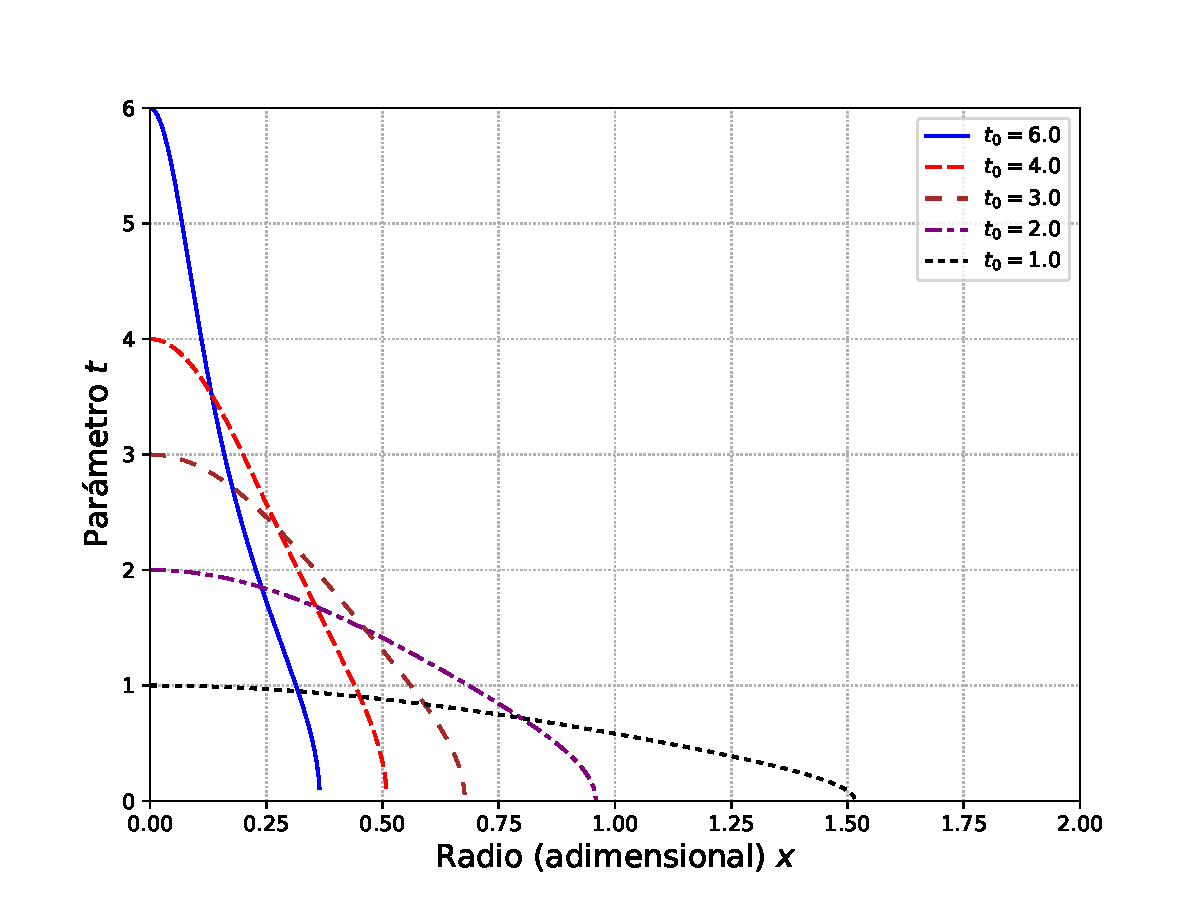
\includegraphics[angle=0,width=0.45\textwidth]{fig/fig-fermi-rel-t-x.pdf}
\figcaption{Soluci'on de ec. TOV: $t$ v/s $x$.}
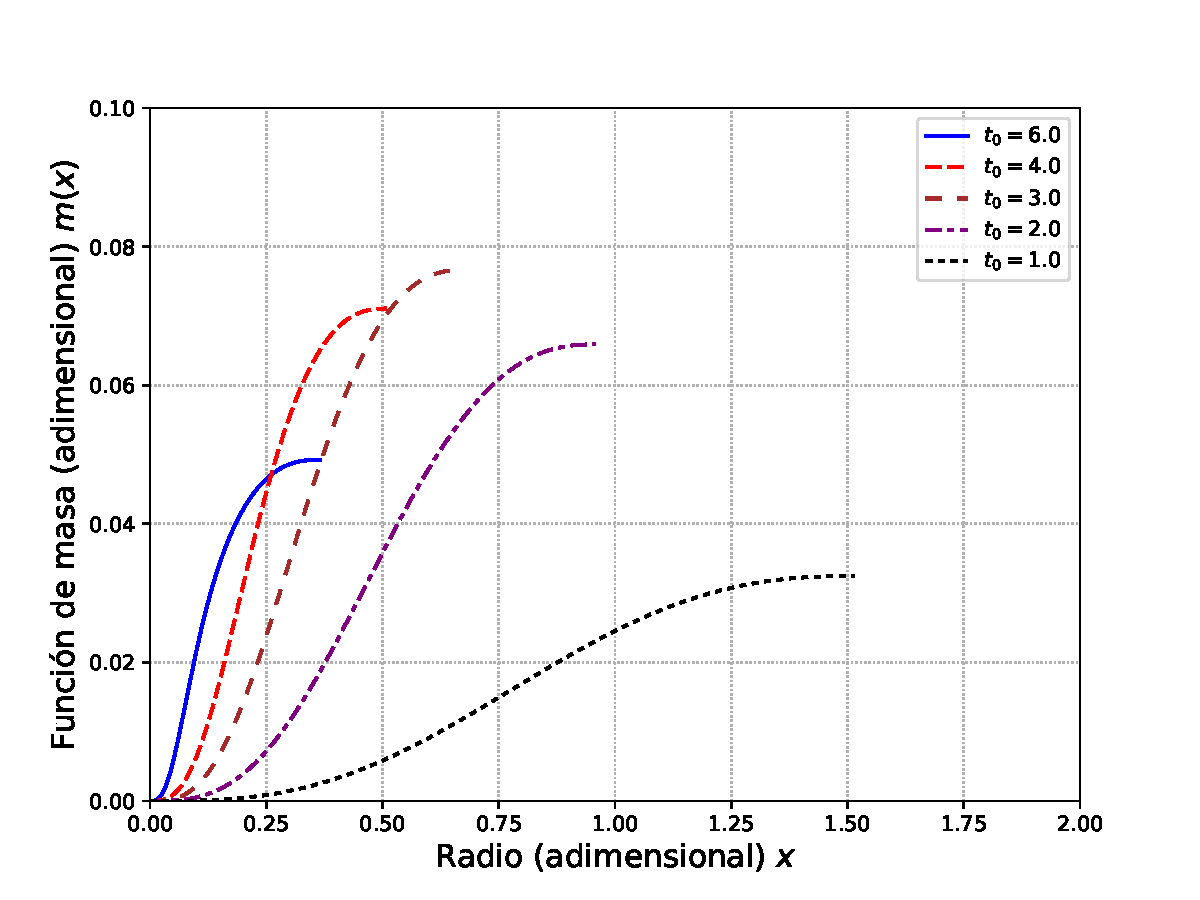
\includegraphics[angle=0,width=0.45\textwidth]{fig/fig-fermi-rel-m-x.pdf}
\figcaption{Soluci'on de ec. TOV: $m$ v/s $x$.}
\end{multicols}

Una caracter'istica que llama en seguida la atenci'on del gr'afico $m$ v/s $x$ es que la masa $m$ se incremente con $t_0$ hasta un cierto valor m'aximo, tras el cual disminuye. En variables f'isicas, esto significa que existe un m'aximo de la masa $M$ con respecto a la densidad central de una estrella de neutrones $\rho_{\rm c}=\rho(t_0)$. Podemos representar esta relaci'on resolviendo el sistema de ecuaciones un n'umero suficiente de veces (500 en nuestro caso), con los valores de la condici'on inicial entre $t_0=0.1$ a $t_0=7$, obteniendo as'i los valores de $x_1$ necesarios para determinar la masa $M$ seg'un \eqref{fermi-rel-masa}. Por otra parte, por cada valor de $t_0$ tendremos que la densidad central estar'a dada al evaluar $\epsilon$ dado por \eqref{fermi-energia-OV} en dicho punto (dividido por $c^2$):
\begin{align}
\rho_{\rm c}=\frac{\epsilon_{n}}{c^2}&=\frac{\pi m_{n}^4c^3}{4h^3}\left(\senh t_0-t_0\right)\\
&\approx5.725\cdot10^{17}\left(\senh t_0-t_0\right)\,[kg/m^3].
\end{align}
As'i, se obtiene el siguiente gr'afico:

\begin{figure}[H]
\centering
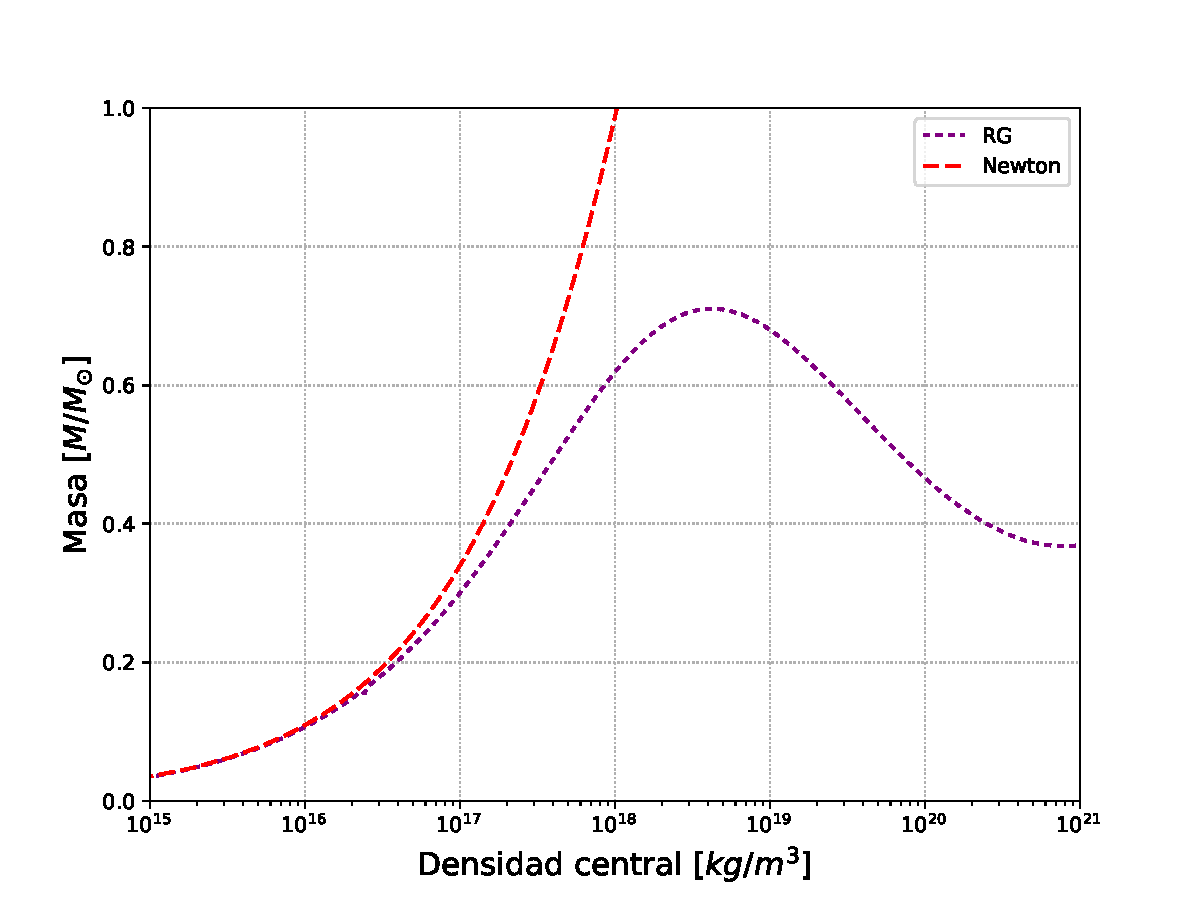
\includegraphics[angle=0,width=0.7\textwidth]{fig/fig-fermi-rel-masa-densidad.pdf}
\caption{Relaci'on masa-densidad central para estrellas de neutrones con las ecuaciones TOV y newtonianas}\label{grafico-fermi-rel-masa-densidad}
\end{figure}
Tambi'en podemos representar la relaci'on masa radio que resulta de la ecuaci'on TOV, para la cual simplemente graficamos los valores de $R$ y $M$ que entregan las relaciones \eqref{fermi-rel-radio} y \eqref{fermi-rel-masa} por cada $x_1$ correspondiente a un $t_0$ dado. Esto se muestra en la siguiente figura, en donde adem'as se grafican los correspondientes resultados newtonianos y el radio de Schwarzchild $R$ correspondiente por cada $M$:

\begin{align}
 R_S&=\frac{2G}{c^2}M\\
&\approx 2.954 \left(\frac{M}{M_{\odot}}\right)\;[km]
\end{align}

\begin{multicols}{2}
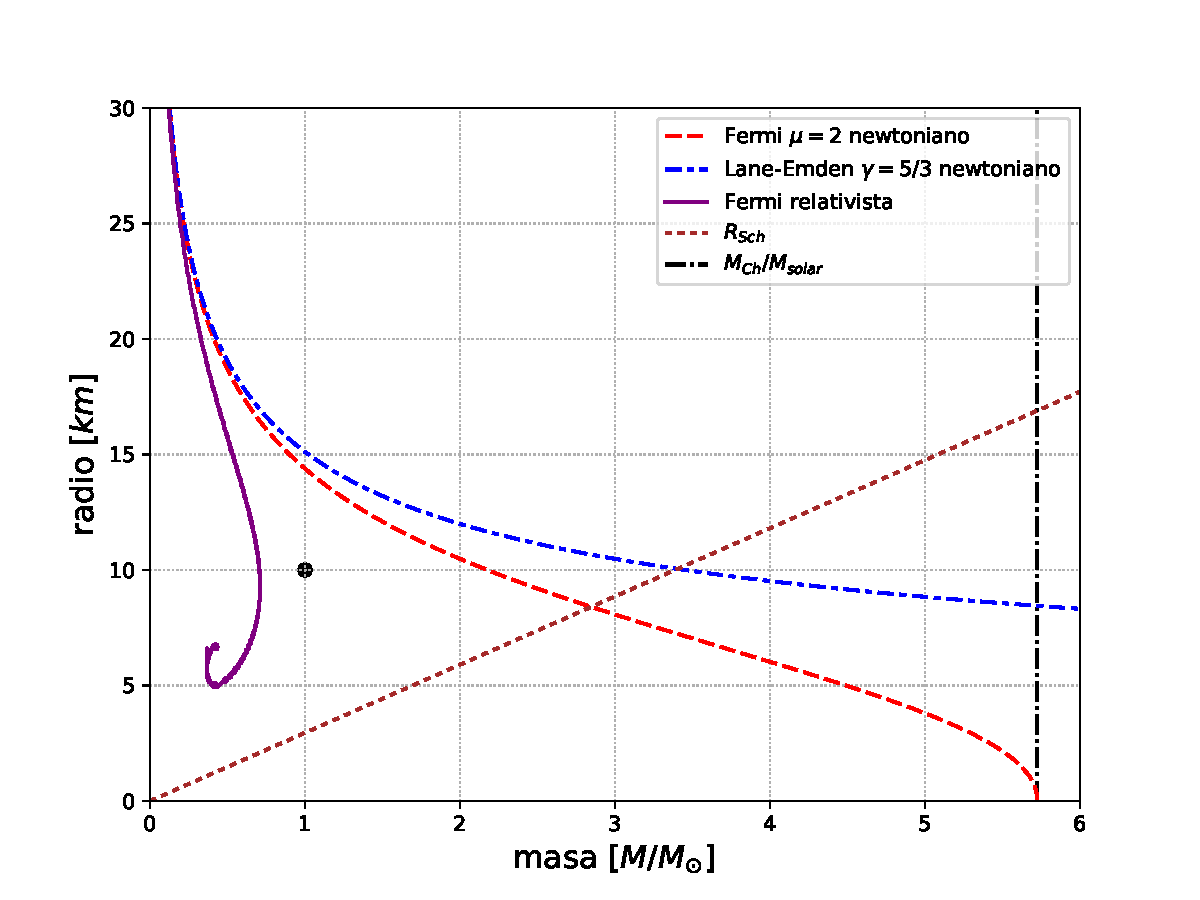
\includegraphics[angle=0,width=0.45\textwidth]{fig/fig-fermi-rel-masa-radio.pdf}
\figcaption{Relaci'on Masa-Radio para estrellas de neutrones con las ecuaciones TOV y newtonianas}
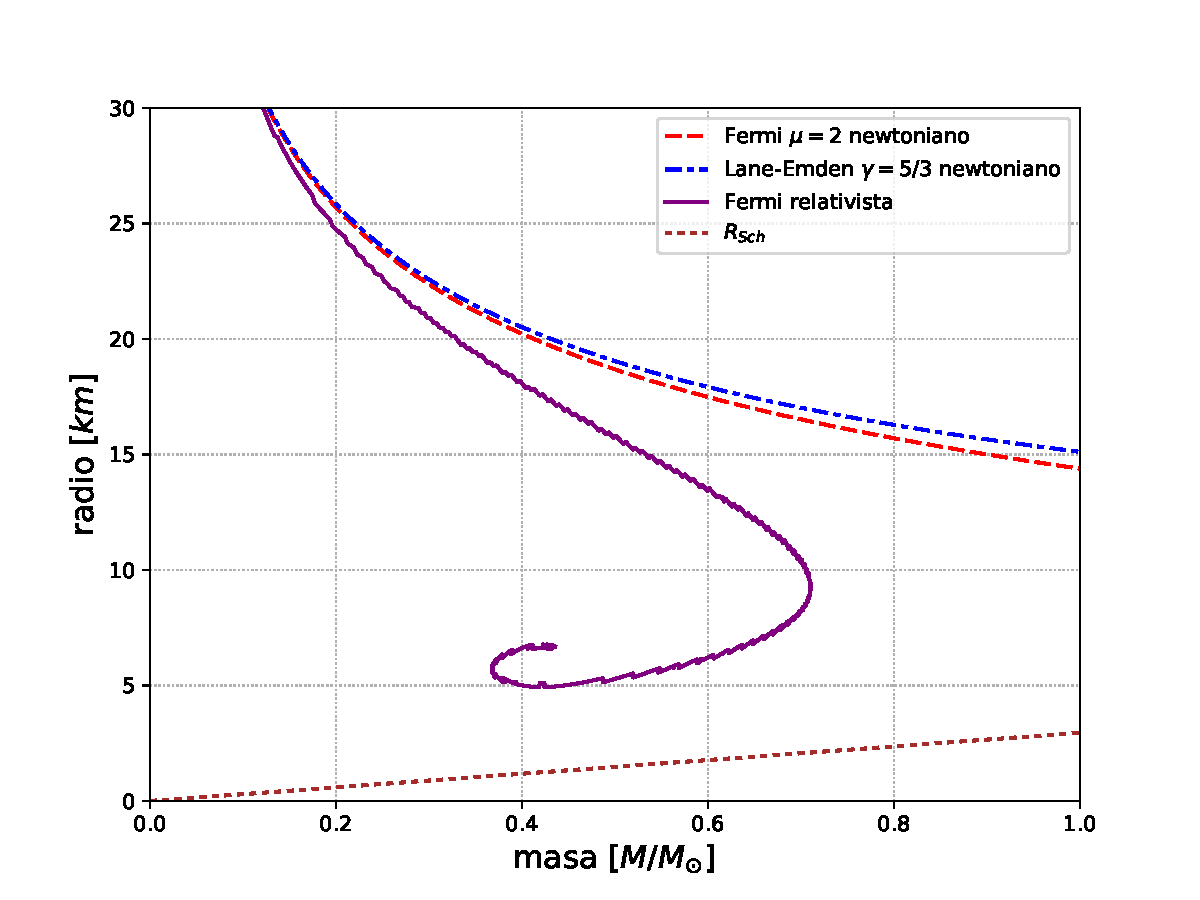
\includegraphics[angle=0,width=0.45\textwidth]{fig/fig-fermi-rel-masa-radio-b.pdf}
\figcaption{Relaci'on Masa-Radio para estrellas de neutrones con las ecuaciones TOV y newtonianas}
\end{multicols}

%\subsection{Masa Gravitacional  \texorpdfstring{$\mathcal{M}$}{M}}\label{sec:masagravitacional}
%% Interpretaci'on de la masa-energ'ia gravitacional. Ver Gravitation \cite{Misner73}
%La definici'on de masa gravitacional total $M$, a partir de su equivalente newtoniano \eqref{masa2},
%\begin{equation}\label{masa_gravitacional}
%\boxed{ M:=\mathcal{M}(R)=\int\limits_0^R4\pi r^2\,\rho(r)\,dr=\int\limits_V \rho(r)\;r^2\sen\theta\,dr\, d\theta\, d\varphi=\int\limits_V \rho(r) dV,}
%\end{equation}
%incluye  todas las formas de energ'ia de la estrella, incluyendo en particular su energ'ia en reposo y la energ'ia del campo gravitacional que produce. Para poder justificar esto, antes es necesario definir algunas cantidades. La primera de ellas es el escalar densidad num'erica de bariones $n$, extendiendo la definici'on \eqref{densidadbarionica} para incluir dependencia radial:
%\begin{equation}
% n(r)=\frac{d\mathcal{N}(r)}{d\mathcal{V}}\quad\Rightarrow\quad\mathcal{N}(r)=\int_{\mathcal{V}}n(r)d\mathcal{V}\label{variacional_numbariones0}
%\end{equation}
%en donde $\mathcal{N}(r)$ (que tambi'en es un escalar) es el n'umero de bariones al interior del volumen propio de la estrella $\mathcal{V}$. El diferencial de esta cantidad se obtendr'a a partir de la relaci'on siguiente en funci'on de $g_{\mu\nu}^3$, la m'etrica esf'erica (dada en \eqref{dsoriginal}) de la hipersuperficie tridimensional con $t=cte$:
%\begin{align}
% d\mathcal{V}&=\sqrt{|det(g_{\mu\nu}^3)|}dx^1dx^2dx^3\\
%&=\sqrt{|(-e^{\beta})(-r^2)(-r^2\sen^2\theta)|}dr d\theta d\varphi,\\
%&=e^{\beta/2}r^2\sen\theta dr\,d\theta\, d\varphi,\\
%&=\left(1-\frac{2G\mathcal{M}}{c^2 r}\right)^{-1/2}r^2\sen\theta\, dr\,d\theta\, d\varphi,\label{volumen_propio}
%\end{align}
%en donde se ha utilizado el coeficiente m'etrico $\beta$ dado en \eqref{beta}. Entonces, podemos determinar el n'umero total de bariones en la estrella reemplazando \eqref{volumen_propio} en la expresi'on \eqref{variacional_numbariones0} evaluada en el radio estelar $r=R$,  de donde al integrar en las variables angulares obtenemos que:
%\begin{equation}\label{variacional_numbariones}
% N=\int_0^R 4\pi r^2 n(r)\left(1-\frac{2G\mathcal{M}}{c^2 r}\right)^{-1/2}dr.
%\end{equation}
%A partir de esta definici'on, podemos encontrar una expresi'on razonable para la masa en reposo total de la estrella, que vendr'ia dada, al usar \eqref{masa_reposo}, por:
%\begin{equation}\label{masatotal_reposo}
% \boxed{M_0:=m_b N=\int_0^R\rho_0(r)\,d\mathcal{V}=\int_0^R 4\pi r^2 \rho_0(r)\left(1-\frac{2G\mathcal{M}}{c^2 r}\right)^{-1/2}dr.}
%\end{equation}
%Esta cantidad, o m'as propiamente $E_0=M_0c^2$, es la energ'ia que la materia de la estrella tendr'ia si fuera dispersada al infinito. Es interesante comparar la relaci'on anterior con \eqref{masa_gravitacional}.
%%Comunmente separalo, hyphenation?
%Con estas relaciones es posible definir una expresi'on razonable para la cantidad com'unmente conocida como la ``energ'ia de la estrella'' $E$, pues restando \eqref{masatotal_reposo} de \eqref{masa_gravitacional}, obtenemos la masa-energ'ia total de la estrella excluyendo masa en reposo. Esta cantidad, multiplicada por $c^2$,
%\begin{align}\label{energia_relativista0}
%E:=(M-M_0)c^2&=(M-m_B\,N)c^2,\\
%&=\int_0^R 4\pi r^2\,dr\,c^2\left\{\rho(r)-\rho_0(r)\left(1-\frac{2G\mathcal{M}(r)}{c^2 r}\right)^{-1/2}\right\},\label{energia_relativista1}
%\end{align}
%tiene la agradable propiedad que es posible separarla en una energ'ia interna y en una energ'ia potencial gravitatoria, que dentro del l'imite apropiado, se reducen a las expresiones newtonianas conocidas. En efecto, de la primera ley de la Termodin'amica tenemos la ecuaci'on \eqref{energia_interna_y_densidad} que relaciona la densidad de energ'ia interna $u$ con $\rho$ y $\rho_0$. Esta relaci'on es independiente en el sentido que no puede deducirse directamente de \eqref{energia_relativista0} como pudiera creerse a simple vista, debido a que las integrales que all'i aparecen difieren en sus elementos de volumen por un factor $e^{\beta/2}$. Luego, reemplazando \eqref{energia_interna_y_densidad} en \eqref{energia_relativista1}, podemos eliminar $\rho_0$ y obtener:
%\begin{align}
% E&=\int_0^R 4\pi r^2\,dr\left\{\rho(r)c^2+\left[u(r)-\rho(r)c^2\right]\left(1-\frac{2G\mathcal{M}(r)}{c^2 r}\right)^{-1/2}\right\}\\
%&=\int_0^R 4\pi r^2\,dr\left\{\,u(r)\,\left(1-\frac{2G\mathcal{M}(r)}{c^2 r}\right)^{-1/2}+\rho(r)c^2\left[1-\left(1-\frac{2G\mathcal{M}(r)}{c^2 r}\right)^{-1/2}\right]\right\}\\
%&=U+V
%\end{align}
%en donde se define la energ'ia interna total $U$ de la estrella como:
%\begin{align}\label{energia_interna_rel_exacta}
% \boxed{U:=\int_0^R 4\pi r^2\,u(r)\,\left(1-\frac{2G\mathcal{M}(r)}{c^2 r}\right)^{-1/2}dr,}
%\end{align}
%mientras que la energ'ia potencial gravitatoria se definir'a por:
%\begin{align}\label{energia_potencial_rel_exacta}
%\boxed{V:=\int_0^R 4\pi r^2\,\rho(r)c^2\left[1-\left(1-\frac{2G\mathcal{M}(r)}{c^2 r}\right)^{-1/2}\right]\,dr.}
%\end{align}
%Ahora, si consideramos como par'ametro de expansi'on la cantidad $G\mathcal{M}/(c^2r)$, podemos notar que el desarrollo en series de ambas definiciones de energ'ia anteriores ser'a:
%\begin{align}\label{energia_interna_rel_approx}
% U&=\int_0^R 4\pi r^2\,u(r)\,\left[1+\frac{G\mathcal{M}(r)}{c^2 r}-\frac{3}{2}\left(\frac{G\mathcal{M}(r)}{c^2 r}\right)^2+\cdots\right]dr,\\
%V&=-\int_0^R 4\pi r^2\,\rho(r)\left[\frac{G\mathcal{M}(r)}{ r}+\frac{3}{2c^2}\left(\frac{G\mathcal{M}(r)}{r}\right)^2+\cdots\right]\,dr.\label{energia_potencial_rel_approx}
%\end{align}
%Como se mencion'o, estas expresiones coinciden con sus correspondientes definiciones newtonianas al considerarlas a primer orden en $\mathcal{M}(r)$ y en $u(r)$, puesto que en dicho caso:
%\begin{align}
% U&\approx\int_0^R (4\pi r^2\,dr)\,u(r)=\int_0^R \,u(r)\,dV\\
%V&\approx-\int_0^R (4\pi r^2\,dr)\rho(r)\frac{G\mathcal{M}(r)}{r}=-\int_0^R(\rho_0\, dV)\frac{G\mathcal{M}(r)}{r}=-\int_0^R\frac{G\mathcal{M}(r)}{r}d\mathcal{M},
%\end{align}
%que corresponden a \eqref{energia_interna_newton} y \eqref{energia_potencial_newton}, respectivamente. N'otese que en las relaciones anteriores se ha usado el hecho que en el caso newtoniano, la densidad de masa-energ'ia total $\rho$ est'a dominada por la densidad de masa en reposo $\rho_0$, de donde se tendr'a que $\rho\approx \rho_0=m_b n$, y por la ecuaci'on \eqref{energia_interna_y_densidad} la energ'ia interna ser'a despreciable en comparaci'on con estos t'erminos. Adem'as se ha utilizado, consistemente con la discusi'on previa y en analog'ia a \eqref{masa1}, la relaci'on $d\mathcal{M}(r)/dV=\rho_0(r)$.
%
%Finalmente, usando las expresiones \eqref{energia_relativista0} y las definiciones \eqref{energia_interna_rel_exacta}, \eqref{energia_potencial_rel_exacta} y \eqref{masatotal_reposo}, podemos escribir una descomposici'on para $M$ de la siguiente forma:
%\begin{equation}\label{energia_separacion}
% \boxed{Mc^2=M_0 c^2+E=M_0 c^2+U+V.}
%\end{equation}
%De aqu'i podemos ver m'as claramente la afirmaci'on hecha al principio de esta secci'on: $Mc^2$ se puede considerar como la suma de la energ'ia en reposo de la materia de la estrella, adem'as de su energ'ia interna y la  energ'ia del campo gravitacional. Esto sucede a pesar que en la definici'on de $M$ est'e presente 'unicamente la densidad de masa-energ'ia de la materia $\rho$.
%
%Es importante notar que la descomposici'on hecha en \eqref{energia_separacion} de la distribuci'on de masa-energ'ia de la materia y su campo gravitacional es 'unicamente v'alida para un sistema esf'ericamente sim'etrico, tal como la estrella que modela. En general, debido a que el tensor energ'ia-momentum del campo gravitacional no es 'unico, \emph{no} es posible efectuar dicha descomposici'on para un sistema arbitrario\footnote{El problema no radica en la existencia de la energ'ia gravitacional, sino m'as bien en su no localizibilidad, pues el principio de equivalencia lo prohibe: siempre existir'a un sistema de referencia localmente inercial en el cual el campo gravitacional se anule ($\Gamma_{\mu\nu}^{\alpha}=0$), lo que implica que la energ'ia del campo tambi'en se anular'a en dicho SR, pero no necesariamente en otro.}. Pero en este caso, a pesar que esa afirmaci'on sigue teniendo validez, es posible seleccionar una distribuci'on de masa-energ'ia total que es f'isicamente razonable: $M$, lo que es avalado por \eqref{energia_separacion} y debido tambi'en a que en el caso newtoniano e posible identificarla con la masa total de una estrella, seg'un \eqref{masa1}. Adem'as, existe otra raz'on que justifica esta elecci'on: $M$ corresponde a la definici'on operacional de masa de una estrella usada en Astrof'isica, esto es, la obtenida de la tercera ley de Kepler ($M=\omega^2 a^3$) a partir de la medici'on del semieje mayor $a$ y periodo $\omega$ de un astro (un planeta u otra estrella en un sistema binario) que orbita en una trayectoria el'iptica en torno a la estrella considerada\footnote{Para mayores detalles, ver cap'itulo 23 del texto \cite{Misner73}.}.
%
%
%\section[Principio variacional para ec. TOV]{Ecuaci'on de estructura relativista de un principio variacional}\label{sec:ppio_variacional_rel}
%En esta secci'on se probar'a el an'alogo relativista (ver secci'on \ref{sec:ppio_variacional_newton} para el caso newtoniano) de la derivaci'on de las ecuaci'on de estructura de Tolman-Oppenheimer-Volkoff a partir de un principio variacional, tomando en cuenta las variaciones eulerianas de las variables del fluido. Esto es, se extremar'a el equivalente a la energ'ia total newtoniana $E$ del fluido, correspondiente a  $M$ (dado por \eqref{masa_gravitacional}), sujeto a la restricci'on de n'umero de bariones $N$ constante. Para encontrar dicho valor estacionario con respecto a todas las variaciones de $\rho(r)$ \footnote {Cada una de ellas representa una configuraci'on de equilibrio si existe una ecuaci'on de estado que relacione el perfil de densidad $\rho(r)$ con la presi'on $P(r)$ y densidad de bariones $n(r)$.} con $N$ constante, se utilizar'a el m'etodo de multiplicadores de Lagrange, que establece que la afirmaci'on anterior se cumplir'a si y s'olo si existe una constante $\lambda$ tal que la siguiente cantidad sea un extremo con respecto a variaciones arbitrarias de $\rho(r)$, pero ahora \emph{sin} restricciones.
%\begin{equation}
% M-\lambda N=\int_0^R 4\pi r^2\,dr\left\{\rho(r)-\lambda n(r)\,e^{\beta(r)/2}\right\}.
%\end{equation}
%De este modo, el valor estacionario de la cantidad anterior se obtendr'a a partir de\footnote{Notar que la variaci'on de $M-\lambda N$, por la ecuaci'on \eqref{energia_relativista0}, equivale a tomar la variaci'on de $E/c^2$, en donde el multiplicador de Lagrange $\lambda$ corresponde a la masa de un bari'on $m_B$}:
%\begin{align}
% \delta M-\lambda\delta N&=\int_0^R 4\pi r^2\,dr\left\{\delta\rho(r)-\lambda \delta\left[n(r)\,\left(1-\frac{2G\mathcal{M}}{c^2 r}\right)^{-1/2}\right]\right\}\\
%&=\int_0^R 4\pi r^2\,dr\left\{\delta\rho(r)-\lambda \delta n(r)\left(1-\frac{2G\mathcal{M}}{c^2 r}\right)^{-1/2}-n(r)\delta\left[\left(1-\frac{2G\mathcal{M}}{c^2 r}\right)^{-1/2}\right]\right\}\\
%&=\int_0^R 4\pi r^2\,dr\left\{\delta\rho(r)-\lambda \delta n(r)\left(1-\frac{2G\mathcal{M}}{c^2 r}\right)^{-1/2}-\frac{\lambda Gn(r)}{c^2 r} \delta\mathcal{M}(r)\left(1-\frac{2G\mathcal{M}}{c^2 r}\right)^{-3/2}\right\}\label{variacional_c1}
%\end{align}
%Ahora se debe encontrar una relaci'on entre $\delta \rho$ y $\delta n$ que permita expresar el segundo t'ermino de la ecuaci'on anterior \eqref{variacional_c1} en funci'on de $\delta\rho$, para lo cual recurrimos a la relaci'on obtenida de la primera ley de la Termodin'amica en el caso de entrop'ia por bari'on constante \eqref{1leytermo}, cambiando los diferenciales $d$ por variaciones $\delta$:
%\begin{equation}\label{variacional_c2}
% \delta n(r)=\frac{n(r)}{P(r)+\rho(r)c^2}\delta\rho(r) c^2.
%\end{equation}
%Luego, s'olo falta expresar el tercer t'ermino de \eqref{variacional_c1} en t'erminos de $\delta\rho$, para lo cual reescribimos $\delta\mathcal{M}$ usando su definici'on de \eqref{masa2}:
%\begin{align}
% \delta\mathcal{M}(r)=\int_0^r 4\pi r'^2\delta\rho(r')dr'.\label{variacional_c3}
%\end{align}
%De esta forma, reemplazando \eqref{variacional_c2} y \eqref{variacional_c3} en \eqref{variacional_c1}, podemos escribir las tres integrales s'olo en funci'on de variaciones en $\delta\rho$:
%\begin{align}
% \delta M-\lambda \delta N&=\int_0^R 4\pi r^2\delta \rho\,dr\left\{1-\frac{\lambda n(r)c^2}{P(r)+\rho(r)c^2} \left(1-\frac{2G\mathcal{M}}{c^2 r}\right)^{-1/2}\right\}\\
%&\quad-\frac{\lambda G}{c^2} \int_0^R 4\pi r\,dr\left(1-\frac{2G\mathcal{M}}{c^2 r}\right)^{-3/2}n(r)\int_0^r 4\pi r'^2\delta\rho(r')dr'\label{variacional_c4}
%\end{align}
%La 'ultima integral se puede reescribir simb'olicamente como una funci'on $f=f(r,r')$ integrada en el dominio se\~nalado (ver figura...), a la cual podemos invertir el orden de las variables de integraci'on:
%\begin{align}
% \int\limits_{r=0}^{r=R}dr\int\limits_{r'=0}^{r'=r}dr'\,f(r,r')=\int\limits_{r'=0}^{r'=R}dr'\int\limits_{r=r'}^{r=R}dr\,f(r,r')=\int\limits_{r=0}^{r=R}dr\int\limits_{r'=r}^{r'=R}dr\,f(r',r),
%\end{align}
%en donde en la 'ultima igualdad simplemente se han renombrado las variables de integraci'on. De este modo, la integral original indicada se puede reescribir como:
%\begin{align}
%&\frac{\lambda G}{c^2} \int_0^R 4\pi r\left(1-\frac{2G\mathcal{M}(r)}{c^2 r}\right)^{-3/2}n(r)\int_0^r 4\pi r'^2\delta\rho(r')dr'\\
%&=\int_0^R 4\pi r^2\left\{ \frac{\lambda G}{c^2}\int_r^R 4\pi r' n(r') \left(1-\frac{2G\mathcal{M}(r')}{c^2 r}\right)^{-3/2}dr'\right\}\delta\rho(r)dr.
%\end{align}
%Por lo tanto, \eqref{variacional_c4} equivaldr'a a:
%\begin{align}
% \delta M-\lambda \delta N&=\int_0^R 4\pi r^2\delta \rho\,dr\left\{1-\frac{\lambda n(r)c^2}{P(r)+\rho(r)c^2} \left(1-\frac{2G\mathcal{M}}{c^2 r}\right)^{-1/2}-\frac{\lambda G}{c^2}\int_r^{\infty} 4\pi r' n(r') \left(1-\frac{2G\mathcal{M}}{c^2 r}\right)^{-3/2}dr'\right\}.
%\end{align}
%Esta variaci'on se anular'a para todo $\delta\rho$ si y s'olo si el integrando anterior es id'enticamente nulo, de donde se podr'a despejar $\lambda$:
%\begin{align}
%&1-\lambda\left\{\frac{ n(r)c^2}{P(r)+\rho(r)c^2} \left(1-\frac{2G\mathcal{M}}{c^2 r}\right)^{-1/2}+\frac{ G}{c^2}\int_r^{\infty} 4\pi r' n(r') \left(1-\frac{2G\mathcal{M}}{c^2 r}\right)^{-3/2}dr'\right\}=0\\
%\Rightarrow\quad\frac{1}{\lambda}&=\frac{ n(r)c^2}{P(r)+\rho(r)c^2} \left(1-\frac{2G\mathcal{M}}{c^2 r}\right)^{-1/2}+\frac{ G}{c^2}\int_r^{\infty} 4\pi r' n(r') \left(1-\frac{2G\mathcal{M}}{c^2 r}\right)^{-3/2}dr'.
%\end{align}
%Pero el multiplicador de Lagrange $\lambda$ es constante, y en particular independiente de la coordenada radial, por lo que su derivada con respecto a $r$ deber'a anularse:
%\begin{align}
% 0&=\frac{\partial}{\partial r}\left(\frac{1}{\lambda}\right)=\frac{d}{dr}\left[\frac{ n(r)c^2}{P(r)+\rho(r)c^2}\right] \left(1-\frac{2G\mathcal{M}}{c^2 r}\right)^{-1/2}+\frac{n(r)c^2}{P(r)+\rho(r)c^2}\frac{d}{dr} \left(1-\frac{2G\mathcal{M}}{c^2 r}\right)^{-3/2}\\
%&\quad-\frac{ G}{c^2}4\pi r n(r) \left(1-\frac{2G\mathcal{M}}{c^2 r}\right)^{-3/2}\\
%&=\left[\frac{n'}{P+\rho c^2}-\frac{n(P'+\rho' c^2)}{(P+\rho c^2)^2}\right]c^2\left(1-\frac{2G\mathcal{M}}{c^2 r}\right)^{-1/2}\\
%&\quad+\frac{Gn}{P+\rho c^2}\left[\mathcal{M}'\frac{1}{r}-\frac{\mathcal{M}}{r^2}\right] \left(1-\frac{2G\mathcal{M}}{c^2 r}\right)^{-3/2}-\frac{ 4\pi G r}{c^2} n\left(1-\frac{2G\mathcal{M}}{c^2 r}\right)^{-3/2}\label{variacional_c5}.
%\end{align}
%La derivada de la masa parcial $\mathcal{M}$ se puede reemplazar por su definici'on \eqref{masa1}, mientras que el primer t'ermino en par'entesis cuadrado se logra simplificar al utilizar nuevamente la primera ley de la Termodin'amica \eqref{1leytermo} (tambi'en con $s=cte$), ahora en forma de derivada radial:
%\begin{align}
%\frac{\rho c^2+P}{n}\frac{dn}{dr} &=\frac{d\rho}{dr}c^2\\
%\Rightarrow \quad n'\left(P+\rho c^2\right)-n(\rho'c^2)&=0.
%\end{align}
%De este modo, el primer t'ermino en par'entesis cuadrado en \eqref{variacional_c5} ser'a equivalente a:
%\begin{align}
%\left[\frac{n'}{P+\rho c^2}-\frac{n(P'+\rho' c^2)}{(P+\rho c^2)^2}\right]&=\frac{n'(P+\rho c^2)-n\rho' c^2-nP'}{(P+\rho c^2)^2}\\
%&=-\frac{nP'}{(P+\rho c^2)^2}.
%\end{align}
%Luego, usando las expresiones indicadas, encontramos que de \eqref{variacional_c5} se pueden eliminar todas las derivadas radiales excepto la correspondiente a la presi'on $P'$, por lo que tendremos:
%\begin{align}
% 0&=c^2\left[-\frac{nP'}{(P+\rho c^2)^2}\right]\left(1-\frac{2G\mathcal{M}}{c^2 r}\right)^{-1/2}+\frac{Gn}{P+\rho c^2}\left[\left(4\pi r^2\rho\right)\frac{1}{r}-\frac{\mathcal{M}}{r^2}\right] \left(1-\frac{2G\mathcal{M}}{c^2 r}\right)^{-3/2}\\
%&\quad-\frac{ 4\pi G r}{c^2} n\left(1-\frac{2G\mathcal{M}}{c^2 r}\right)^{-3/2}.
%\end{align}
%Multiplicando por $\left(1-\frac{2G\mathcal{M}}{c^2 r}\right)^{-1/2}$ y $(P+\rho c^2)^2$, podemos despejar $P'$, obteniendo:
%\begin{align}
%P'c^2&=(P+\rho c^2)\left[4\pi G r\rho -\frac{G\mathcal{M}}{r^2}\right]\left(1-\frac{2G\mathcal{M}}{c^2 r}\right)^{-1}-\frac{4\pi G r}{c^2}(P+\rho c^2)^2\left(1-\frac{2G\mathcal{M}}{c^2 r}\right)^{-1}\\
%&=\left(1-\frac{2G\mathcal{M}}{c^2 r}\right)^{-1}(P+\rho c^2)\left[\cancel{4\pi G r\rho}-\frac{G\mathcal{M}}{r^2}-\frac{4\pi G r}{c^2}\left(P+\cancel{\rho c^2}\right)\right],\\
%\Rightarrow\quad P'&=-\frac{G\mathcal{M}\rho}{r^2}\left(1+\frac{P}{\rho c^2}\right)\left(1+\frac{4\pi r^3 P}{\mathcal{M}c^2}\right)\left(1-\frac{2G\mathcal{M}}{c^2 r}\right)^{-1}.
%\end{align}
%que es la ecuaci'on TOV \eqref{tov} de un modelo estelar relativista en equilibrio, tal como se quer'ia probar.
%
%\section[Inestabilidad relativista]{Inestabilidad relativista obtenida de un principio variacional}
%
%En esta secci'on se mostrar'a una inestabilidad debida netamente a efectos de Relatividad General que se presenta en ciertos tipos de enanas blancas. Se deducir'a de forma similar al m'etodo usado para hallar el criterio del 'indice politr'opico $\gamma$ de la secci'on \ref{sec:criterio_indicegamma}, es decir, extremando la energ'ia para encontrar la configuraci'on de equilibrio y a partir de dicha informaci'on determinar cu'ales de ellas son estables. El resultado que se encontrar'a es que la diferencia en la energ'ia con respecto al caso newtoniano implicar'a una restricci'on m'as fuerte sobre  $\gamma$ para una soluci'on estable, lo que se puede entender en base a las discusiones previas: Relatividad General tiende a desestabilizar modelos estelares en comparaci'on con el caso newtoniano.
%
%Para encontrar dicho efecto, primero se debe determinar la energ'ia de una estrella en Relatividad General. Se supondr'a que la ecuaci'on de estado del fluido ideal es politr'opica, dada por \eqref{estadopolitropica_general} con un 'indice $\gamma$ cercano a $4/3$. As'i, en primera aproximaci'on con respecto a Newton, la energ'ia estelar se puede escribir como
%\begin{equation}\label{energia_total1}
% E=U+V+\Delta U+\Delta E_{RG},
%\end{equation}
%en donde $U$ es la energ'ia interna newtoniana para un fluido con ecuaci'on de estado politr'opica $P=K\rho_0^{4/3}$, $\Delta U$ es la correci'on de dicha energ'ia para tomar en cuenta ecuaciones de estado cercanas con $\gamma\sim 4/3$, $V$ es la energ'ia potencial gravitatoria newtoniana, y $\Delta E_{RG}$ representa la correcci'on a la energ'ia total newtoniana debida a efectos de Relatividad General. A continuaci'on se determinar'a por separado los dos 'ultimos t'erminos.
%
%\subsection{Correcci'on de la energ'ia total por R.G.: \texorpdfstring{$\Delta E_{RG}$}{Delta E-RG}}
%La diferencia de energ'ia de una estrella politr'opica que se calcular'a en esta subsecci'on ser'a
%\begin{equation}
%\Delta E_{RG}=E_{RG}-E_{NW},
%\end{equation}
%en donde $E_{RG}$ es la energ'ia total relativista de la estrella (excluyendo la masa-energ'ia en reposo) dada por \eqref{energia_relativista0} y $E_{NW}$ es la energ'ia newtoniana dada por la suma de \eqref{energia_potencial_newton} y \eqref{energia_interna_newton}. Para determinar el primer t'ermino en una forma apropiada para nuestros fines, primero factorizamos el t'ermino $e^{\beta/2}$ de \eqref{energia_relativista1}:
%\begin{align}
%E_{RG}&=(M-m_B N)c^2\\
%&=\int_0^R \left(1-\frac{2G\mathcal{M}(r)}{c^2 r}\right)^{-1/2}4\pi r^2\,dr\,c^2\left\{\rho(r)\left(1-\frac{2G\mathcal{M}(r)}{c^2 r}\right)^{1/2}-\rho_0(r)\right\}\\
%&=\int_V \left\{\rho(r)c^2\left(1-\frac{2G\mathcal{M}(r)}{c^2 r}\right)^{1/2}-\rho_0(r)c^2\right\}\,d\mathcal{V}.
%\end{align}
%Aqu'i se ha usado la definici'on de volumen propio \eqref{volumen_propio}. Luego, debemos usar la relaci'on entre energ'ia interna $u$, densidad de masa total $\rho$ y densidad de masa en reposo $\rho_0$ dada en  \eqref{energia_interna_y_densidad}, para eliminar $\rho$ (a diferencia de lo realizado en la secci'on \ref{sec:masagravitacional} en donde se elimina $\rho_0$):
%\begin{align}
%E_{RG}&=\int_V \left\{\left[u+\rho_0c^2\right]\left(1-\frac{2G\mathcal{M}}{c^2 r}\right)^{1/2}-\rho_0c^2\right\}\,d\mathcal{V}\\
%&=\int_V \left\{\left[\frac{u}{\rho_0 c ^2}+1\right]\left(1-\frac{2G\mathcal{M}}{c^2 r}\right)^{1/2}-1\right\}\,\rho_0c^2\,d\mathcal{V}.
%\end{align}
%Esta formulaci'on tiene la ventaja que la cantidad $\rho_0\, d\mathcal{V}$ es un invariante (por lo que no se expande). De esta forma, podemos expandir la relaci'on anterior con respecto a $\mathcal{M}/r$ y $u/(\rho c^2)$ hasta cantidades a segundo orden (de forma an'aloga a lo realizado en \eqref{energia_interna_rel_approx} y \eqref{energia_potencial_rel_approx}):
%\begin{align}
% E_{RG}&=\int_V \left\{\left[\frac{u}{\rho_0 c ^2}+1\right]\left[1-\frac{G\mathcal{M}}{c^2 r}-\frac{1}{2}\left(\frac{G\mathcal{M}}{c^2 r}\right)^2+\mathcal{O}(\mathcal{M}^3)\right]-1\right\}\,\rho_0c^2\,d\mathcal{V}\\
%&=\int_V \left\{\frac{u}{\rho_0 c ^2}-\frac{G\mathcal{M}}{c^2 r}-\left(\frac{u}{\rho_0 c ^2}\right)\left(\frac{G\mathcal{M}}{c^2 r}\right)-\frac{1}{2}\left(\frac{G\mathcal{M}}{c^2 r}\right)^2+\mathcal{O}(\mathcal{M}^3)\right\}\,\rho_0c^2\,d\mathcal{V}.\label{energia_rg_1}
%\end{align}
%Ahora, debemos determinar la correspondiente expresi'on newtoniana para la energ'ia $E_{NW}$, dada por la suma de \eqref{energia_interna_newton} y \eqref{energia_potencial_newton}. Sin embargo, dicha energ'ia debe corresponder a la \emph{misma} estrella en ambas formulaciones, por lo cual se debe definir en t'erminos invariantes como la correspondiente a esferas de fluidos politr'opicas que tienen el mismo n'umero de bariones $\mathcal{N}$ en un volumen propio determinado $d\mathcal{V}$ (recordar la ambig\"uedad de coordenadas en Relatividad General). Por esta raz'on, $E_{NW}$ se deber'a escribir como
%\begin{align}
% E_{NW}&=\int\limits_0^R u(r^*)\, d\mathcal{V}(r^*)-\int_M\frac{G\mathcal{M}(r^*)}{r^*}\,d\mathcal{M}(r^*)\\
%&=\int\limits_M \frac{u(r^*)}{\rho_0}\, d\mathcal{M}(r^*)-\int_M\frac{G\mathcal{M}(r^*)}{r^*}\,d\mathcal{M}(r^*)\\
%&=\int\limits_V\left\{\frac{u}{\rho_0c^2}-\frac{G\mathcal{M}^*}{c^2r^*}\right\}\,\rho_0 c^2\,d\mathcal{V}\label{energia_nw_1},
%\end{align}
%en donde la coordenada newtoniana $r^*$ se diferencia de la coordenada radial de curvatura $r$ utilizada en \eqref{energia_rg_1}, en que debe satisfacer la relaci'on con respecto al volumen propio dentro del radio $\mathcal{V}$,
%\begin{equation}\label{volumen_propio_y_r*}
% \mathcal{V}(r^*)=\frac{4\pi}{3} (r^*)^3\qquad\Rightarrow\qquad r^*=\left(\frac{3\mathcal{V}}{4\pi}\right)^{1/3},
%\end{equation}
%y tambi'en la siguiente relaci'on con respecto a la masa dentro de $r^*$: $\mathcal{M}(r^*)$:
%\begin{align}\label{masa_y_r*}
% d\mathcal{M}^{*}:=d\mathcal{M}(r^*)=\rho_0\,d\mathcal{V}.
%\end{align}
%
%\subsubsection{Integral de la correcci'on relativista}
%Por lo tanto, la diferencia de energ'ia buscada, a segundo orden, se conseguir'a restando \eqref{energia_nw_1} de \eqref{energia_rg_1}:
%\begin{align}\label{delta_energia}
% \Delta E_{RG}=E_{RG}-E_{NW}\approx\int\limits_{\mathcal{V}}\left\{-\left(\frac{u}{\rho_0 c ^2}\right)\left(\frac{G\mathcal{M}}{c^2 r}\right)-\frac{1}{2}\left(\frac{G\mathcal{M}}{c^2 r}\right)^2+\frac{G\mathcal{M}^{*}}{c^2r^*}-\frac{G\mathcal{M}}{c^2 r}\right\}\,\rho_0c^2\,d\mathcal{V}.
%\end{align}
%Para poder calcular la integral anterior, primero se debe notar que los dos 'ultimos t'erminos en su integrando se pueden escribir como
%\begin{align}
%\frac{G}{c^2}\left(\frac{\mathcal{M}^*}{r^*}-\frac{\mathcal{M}}{ r}\right)&=\frac{G}{c^2}\left(\frac{\mathcal{M}^*}{r^*}-\frac{\mathcal{M}}{r^*}+\frac{\mathcal{M}}{r^*}-\frac{\mathcal{M}}{r}\right)\\
%&=\frac{G}{c^2}\left(\frac{\mathcal{M}^*-M}{r^*}-\frac{\mathcal{M}\left(r^{*}-r\right)}{r\,r^{*}}\right),\label{delta_energia_2l}
%\end{align}
%de modo que debemos encontrar la diferencia entre las coordenadas radiales $r^*-r$ y de las masas al interior de cada una de ellas, $\mathcal{M}(r^{*})-\mathcal{M}(r)$, para poder determinar \eqref{delta_energia} expl'icitamente.
%
%
%
%\begin{itemize}
% \item \emph{Determinaci'on de $r^*-r$}. Debemos establecer primero la relaci'on entre la coordenada de curvatura $r$ y el volumen propio dentro de  ella $\mathcal{V}(r)$. Por la definici'on de $d\mathcal{V}$ en \eqref{volumen_propio}, tendremos que expandiendo a primer orden en $\mathcal{M}/r$ e integrando primero en las variables angulares y despu'es en la radial:
%\begin{align}
%\mathcal{V}(r)&=\int_{\mathcal{V}} d\mathcal{V}=\int\limits_{r'=0}^{r'=r}\int\limits_{\theta=0}^{\theta=\pi}\int\limits_{\varphi=0}^{\varphi=2\pi}\left(1+\frac{G\mathcal{M}}{c^2 r'}+\mathcal{O}\left(\frac{\mathcal{M}}{r'}\right)^2\right)\,r'^2\sen\theta\, dr'\,d\theta\, d\varphi\\
%&\approx\int\limits_{r'=0}^{r'=r}4\pi\left[r'^2\,dr'+\frac{G\mathcal{M} r'}{c^2}dr'\right]\\
%&=\frac{4\pi r^3}{3}\left[1+\frac{3G}{ c^2r^3}\int\limits_{r'=0}^{r'=r}\mathcal{M}(r')\,r'\,dr'\right]\label{volumen_propio_y_r}.
%\end{align}
%De este modo, podemos reemplazar la expresi'on anterior en \eqref{volumen_propio_y_r*}, que relaciona $\mathcal{V}$ y $r^*$, para obtener, a primer orden, la relaci'on buscada entre las dos coordenadas:
%\begin{align}
%r^*&=\left(\frac{3}{4\pi}\frac{4\pi r^3}{3}\left[1+\frac{3G}{ c^2r^3}\int\limits_{r'=0}^{r'=r}\mathcal{M}(r')\,r'\,dr'\right]\right)^{1/3}\\
%&=r\left[1+\frac{1}{3}\frac{3G}{ c^2r^3}\int\limits_{r'=0}^{r'=r}\mathcal{M}(r')\,r'\,dr'\right]\\
%\Rightarrow\qquad r^*-r&=\frac{G}{ c^2r^2}\int\limits_{r'=0}^{r'=r}\mathcal{M}(r')\,r'\,dr'\label{energia_r_y_r*}.
%\end{align}
%
%
%
%\item \emph{Determinaci'on de $\mathcal{M}(r^{*})-\mathcal{M}(r)$}
%Para ello, primero se reescribe esta 'ultima a partir de su definici'on  \eqref{masa_gravitacional} en t'erminos del volumen propio definido en \eqref{volumen_propio}:
%\begin{align}
%\mathcal{M}(r)&=\int\limits_0^r 4\pi r'^2\,\rho(r')\,dr'=\int\limits_0^r\rho(r)e^{-\beta/2}\left(4\pi r'^2 e^{\beta/2}\,dr\right)\\
%&=\int\limits_0^r\rho(r)\left(1-\frac{2G\mathcal{M}(r)}{c^2 r}\right)^{1/2}\,d\mathcal{V}.
%\end{align}
%Por lo tanto, podremos determinar la diferencia entre ambas definiciones de masa restando la cantidad anterior de $\mathcal{M}(r^*)$, obtenida de integrar \eqref{masa_y_r*}, pues ahora ambas tendr'an en su integrando el elemento de volumen propio $d\mathcal{V}$
%\begin{align}
% \mathcal{M}(r^*)-\mathcal{M}(r)=\int_{\mathcal{V}}d\mathcal{V}\left[\rho_0-\rho(r)\left(1-\frac{2G\mathcal{M}(r)}{c^2 r}\right)^{1/2}\right].
%\end{align}
%Podemos simplificar lo anterior introduciendo la densidad de energ'ia interna $u(r)$ definida en \eqref{energia_interna_y_densidad}, de modo de eliminar la dependencia en la densidad de masa total $\rho(r)$, obteniendo a primer orden en $\mathcal{M}/r$ y $u$:
%\begin{align}
%\mathcal{M}(r^*)-\mathcal{M}(r)&=\int_{\mathcal{V}}d\mathcal{V}\left[\rho_0-\left(\rho_0+\frac{u}{c^2}\right)\left(1-\frac{2G\mathcal{M}(r)}{c^2 r}\right)^{1/2}\right]\\
%&=\int_{\mathcal{V}}\rho_0\,d\mathcal{V}\left[1-\left(1+\frac{u}{\rho_0 c^2}\right)\left(1-\frac{G\mathcal{M}(r)}{c^2 r}+\mathcal{O}\left(\frac{\mathcal{M}}{r}\right)^2\right)\right]\\
%&\approx-\int_{\mathcal{V}}\rho_0\,d\mathcal{V}\left(\frac{u}{\rho_0 c^2}-\frac{G\mathcal{M}(r)}{c^2 r}\right)\label{energia_m_y_m*}.
%\end{align}
%
%\end{itemize}
%Entonces, podemos reemplazar ambas diferencias \eqref{energia_r_y_r*} y \eqref{energia_m_y_m*} en \eqref{delta_energia_2l}, obteniendo:
%\begin{align}
%\frac{G}{c^2}\left(\frac{\mathcal{M}^*}{r^*}-\frac{\mathcal{M}}{ r}\right)&=\frac{G}{c^2}\left\{-\frac{1}{r^{*}}\int_{\mathcal{V}(r)}\rho_0\,d\mathcal{V}\left(\frac{u}{\rho_0 c^2}-\frac{G\mathcal{M}(r)}{c^2 r}\right)-\frac{\mathcal{M}(r)}{rr^{*}}\frac{G}{ c^2r^2}\int\limits_{0}^R\mathcal{M}(r')\,r'\,dr'\right\}.
%\end{align}
%Por lo tanto, reemplazamos estos dos 'ultimos t'erminos del integrando original en la integral \eqref{delta_energia}, obteniendo:
%\begin{align}
%  \Delta E_{RG}&\approx\int\limits_{V}\left\{-\left(\frac{u}{\rho_0 c ^2}\right)\left(\frac{G\mathcal{M}(r)}{c^2 r}\right)-\frac{1}{2}\left(\frac{G\mathcal{M}(r)}{c^2 r}\right)^2\right.\\
%&\quad +\left.\frac{G}{c^4}\left[-\frac{1}{r^{*}}\int_{\mathcal{V}(r)}\rho_0\,d\mathcal{V}\left(\frac{u}{\rho_0}-\frac{G\mathcal{M}(r)}{ r}\right)-\frac{\mathcal{M}(r)}{rr^{*}}\frac{G}{ r^2}\int\limits_{0}^R\mathcal{M}(r')\,r'\,dr'\right]\right\}\,\rho_0c^2\,d\mathcal{V}.
%\end{align}
%La expresi'on anterior se puede simplificar expres'andola en t'erminos s'olo de $r^{*}$ y sus cantidades asociadas, notando que como se han mantenido t'erminos a 2${}^{\circ}$ orden, es posible evaluar la integral con las relaciones \emph{newtonianas} para $\rho_0$, $\mathcal{V}$ y $\mathcal{M}$, pues se consigue un error s'olo a 3${}^{\circ}$ orden. As'i, y usando \eqref{masa_y_r*} para cambiar la variable de integraci'on de $\mathcal{V}(r^*)$ a $\mathcal{M}(r^*)$, tenemos:
%\begin{align}
%  \Delta E_{RG}&\approx\frac{G}{c^2}\int\limits_0^Md\mathcal{M}^{*}\Biggl\{-\frac{u}{\rho_0}\frac{\mathcal{M}^*}{ r^*}-\frac{G}{2}\left(\frac{\mathcal{M}^*}{r^*}\right)^{2}-\frac{1}{r^{*}}\int\limits_0^{\mathcal{M}^*} d\mathcal{M}'\left(\frac{u(r')}{\rho_0(r') }-\frac{G\mathcal{M}(r')}{r'}\right)\Biggr.\\
%&\quad -\Biggl.\frac{G\mathcal{M^*}}{(r^{*})^4}\int\limits_{0}^{r^*}\mathcal{M}(r')\,r'\,dr'\Biggr\}.
%\end{align}
%Separando expl'icitamente las 5 integrales, y renombrando la variable de integraci'on a $r=r^*$, tenemos que la correcci'on de energ'ia relativista est'a dada, a primer orden, por:
%\begin{align}
%   \Delta E_{RG}&\approx\frac{G}{c^2}\Biggl\{-\underbrace{\int\limits_0^M\frac{u}{\rho_0}\frac{\mathcal{M}}{ r}\,d\mathcal{M}}_{:=I_1}-\underbrace{\frac{G}{2}\int\limits_0^M\left(\frac{\mathcal{M}}{r}\right)^{2}d\mathcal{M}}_{:=I_2}-\underbrace{\int\limits_0^M\frac{d\mathcal{M}}{r}\int\limits_0^{\mathcal{M}} \frac{u(r')}{\rho_0(r') }\,d\mathcal{M}'}_{:=I_3}\Biggr.\\
%&\quad +\Biggl.\underbrace{G\int\limits_0^M\frac{d\mathcal{M}}{r}\int\limits_0^{\mathcal{M}}\frac{\mathcal{M}(r')}{r'}\,d\mathcal{M}'}_{:=I_4}-\underbrace{G\int\limits_0^M\frac{\mathcal{M}\,d\mathcal{M}}{r^4}\int\limits_{0}^R\mathcal{M}(r')\,r'\,dr'}_{:=I_5}\Biggr\}.
%\end{align}
%Denotando las integrales de la forma indicada, tendremos que la correci'on de energ'ia buscada se puede escribir como:
%\begin{align}
%	\Delta E_{RG}&\approx\frac{G}{c^2}\left\{ I_1+I_2+I_3+I_4+I_5\right\}\label{delta_energia_2}.
%\end{align}
%
%\subsubsection{Calculando la integral de correcci'on relativista}
%
%Ahora, la idea es obtener relaciones entre las 5 integrales anteriores para expresarlas de una forma m'as compacta.
%
%\begin{itemize}
%\item \emph{Relaci'on entre $I_1$ y $I_5$}\\
%Primero debemos reescribir el primer integrando de $I_5$, para lo cual usamos la ecuaci'on de masa \eqref{masa2}, recordando que $\rho\approx\rho_0$ en la teor'ia newtoniana:
%\begin{align}
% -\frac{\mathcal{M}\,d\mathcal{M}}{r^4}&=4\pi \left(-\frac{\mathcal{M}\rho_0}{r^2}\,dr\right).
%\end{align}
%Ahora podemos introducir la presi'on en la cantidad entre par'entesis usando la ecuaci'on de equilibrio hidrost'atico newtoniano \eqref{eqnewton}, con lo que tenemos:
%\begin{align}\label{energia_myp}
%-\frac{\mathcal{M}\,d\mathcal{M}}{r^4}&= \frac{4\pi}{G}dP.
%\end{align}
%Luego, reemplazando en la integral $I_5$ e integrando por partes, obtenemos:
%\begin{align}
% I_5&=-G\int\limits_0^M\frac{\mathcal{M}\,d\mathcal{M}}{r^4}\int\limits_{0}^R\mathcal{M}(r')\,r'\,dr'\\
%&= \int\limits_{P(r=0)}^{P(r=R)}4\pi\, dP \int\limits_{0}^R\mathcal{M}(r')\,r'\,dr'\\
%&=4\pi\int\limits_{P(r=0)}^{P(r=R)}\left\{d\left(P\int\limits_{0}^R\mathcal{M}(r')\,r'\,dr'\right)-P\mathcal{M}(r')\,r'\,dr'\right\}\\
%&=4\pi\left\{\cancelto{0}{P(R)}\;\int\limits_{0}^R\mathcal{M}(r')\,r'\,dr'-P(0)\cancelto{0}{\int\limits_{0}^{0}\mathcal{M}(r')\,r'\,dr'}\right\}-4\pi\int\limits_{0}^RP\mathcal{M}(r')\,r'\,dr'.
%\end{align}
%Utilizando la ecuaci'on de estado \eqref{estadopolitropica_alterna} para escribir $P$ en funci'on de la energ'ia interna $u$, y considerando nuevamente la ecuaci'on de masa \eqref{eqnewton} para introducir el diferencial $d\mathcal{M}$, tenemos:
%\begin{align}
% I_5&=-4\pi\left(\gamma-1\right)\int\limits_{0}^Ru(r)\mathcal{M}(r)\,r\,dr\\
%&=-\left(\gamma-1\right)\int\limits_{0}^R\frac{u(r)}{\rho_0}\frac{\mathcal{M}(r)}{r}\,d\mathcal{M}.
%\end{align}
%Pero la integral es f'acilmente identificable como $I_1$, por lo que finalmente encontramos la relaci'on:
%\begin{equation}\label{energia_item1}
% I_5=\left(\gamma-1\right)I_1.
%\end{equation}
%
%
%\item \emph{$I_4$ en t'erminos de $I_1$, $I_2$ e $I_5$}\\
%La idea ahora es reescribir el segundo integrando de $I_4$, para lo cual usamos la relaci'on \eqref{energia_myp} multiplicada por $r^3$, e integramos por partes, obteniendo:
%\begin{align}
%I_4&=G\int\limits_0^M\frac{d\mathcal{M}}{r}\int\limits_0^{\mathcal{M}}\frac{\mathcal{M}(r')}{r'}\,d\mathcal{M}'\\
%&=-G\int\limits_0^M\frac{d\mathcal{M}}{r}\int\limits_{P(r'=0)}^{P(r'=r)}\frac{4\pi r'^3}{G}\,dP'\\
%&=-4\pi \int\limits_0^M\frac{d\mathcal{M}}{r}\int\limits_{P(r'=0)}^{P(r'=r)}\left\{d(r'^3\,P')-P'\,d(r'^3)\right\}\\
%&=-4\pi \int\limits_0^M\frac{d\mathcal{M}}{r}\left\{r^3\,P(r)-0-3\int\limits_{r'=0}^{r'=r}P(r')r'^2\,dr'\right\}\\
%&=-4\pi \int\limits_0^M\,Pr^2\,d\mathcal{M}+3\int\limits_0^M\frac{d\mathcal{M}}{r}\int\limits_{r'=0}^{r'=r}P(r')\,4\pi\,r'^2\,dr'.
%\end{align}
%Ahora podemos integrar por partes nuevamente la primera integral, simplificando el resultado con \eqref{energia_myp} (multiplicada por $r^2$) y la ecuaci'on de estado \eqref{estadopolitropica_alterna}. Adem'as, se debe cambiar la variable de integraci'on a $\mathcal{M}$ en la segunda integral usando la ecuaci'on de masa \eqref{masa2}, con lo que tenemos:
%\begin{align}
% I_4&=-4\pi \int\limits_{r=0}^{r=R}\left\{d(Pr^2\,\mathcal{M})-Pd(r^2)\mathcal{M}-\mathcal{M}r^2\,dP\right\}+3\int\limits_0^M\frac{d\mathcal{M}}{r}\int\limits_{r'=0}^{r'=r}P(r')\,\frac{d\mathcal{M}}{\rho_0}\\
%&=-4\pi\left.\cancelto{0}{Pr^2}\right|_{r=0}^{r=R}+2\int\limits_{r=0}^{r=R}P\mathcal{M}4\pi\,r\,dr+\int\limits_{r=0}^{r=R}\mathcal{M}\left(4\pi\,r^2\,dP\right)+3\int\limits_0^M\frac{d\mathcal{M}}{r}\int\limits_{r'=0}^{r'=r}\frac{P(r')}{\rho_0(r')}\,d\mathcal{M}\\
%&=2(\gamma-1)\int\limits_{r=0}^{r=R}u(r)\,\frac{\mathcal{M}}{\rho_0\,r}\left(4\pi\rho_0\,r^2\,dr\right)+\int\limits_{0}^{M}\mathcal{M}\left(-\frac{G\mathcal{M}\,d\mathcal{M}}{r^2}\right)+3(\gamma-1)\int\limits_0^M\frac{d\mathcal{M}}{r}\int\limits_{0}^R\frac{u}{\rho_0}\,d\mathcal{M}   \\
%%
%&=2(\gamma-1)\int\limits_{0}^{M}\frac{u}{\rho_0}\frac{\mathcal{M}}{r}d\mathcal{M}-G\int\limits_{0}^{M}\left(\frac{\mathcal{M}}{r}\right)^2\,d\mathcal{M}+3(\gamma-1)\int\limits_0^M\frac{d\mathcal{M}}{r}\int\limits_{0}^R\frac{u}{\rho_0}\,d\mathcal{M}.
%\end{align}
%As'i, podemos finalmente identificar las integrales como $I_2$, $I_1$ e $I_3$ respectivamente, obteniendo la relaci'on
%\begin{align}\label{energia_item2}
% I_4=-2(\gamma-1)I_1+2I_2-3(\gamma-1)I_3.
%\end{align}
%
%
%\item \emph{$I_3$ en t'erminos de $I_1$, $I_2$ e $I_4$}\\
%Para este caso debemos primero integrar por partes la segunda integral de $I_3$, obteniendo:
%\begin{align}
% \int\limits_{0}^{\mathcal{M}}\frac{u}{\rho_0}\,d\mathcal{M}&=\int\limits_{0}^{\mathcal{M}}\left\{d\left(\frac{u}{\rho_0}\mathcal{M}\right)-\mathcal{M}\,d\left(\frac{u}{\rho_0}\right)\right\}\\
%&=\left(\frac{u(r)}{\rho_0(r)}\mathcal{M}(r)-\frac{u(0)}{\rho_0(0)}\cancelto{0}{\mathcal{M}(0)}\right)-\int\limits_{r'=0}^{r'=r}\mathcal{M}(r')\,d\left(\frac{u(r')}{\rho_0(r')}\right).
%\end{align}
%Usando la ecuaci'on de estado \eqref{estadopolitropica_alterna} y la relaci'on \eqref{relacion_dp}, podemos cambiar la variable de integraci'on a $dP$, de modo que:
%\begin{align}
% \int_{0}^{\mathcal{M}}\frac{u}{\rho_0}\,d\mathcal{M}&=\frac{u\mathcal{M}}{\rho_0}-\frac{1}{\gamma-1}\int\limits_{r'=0}^{r'=r}\mathcal{M}(r')\,d\left(\frac{P(r')}{\rho_0(r')}\right)\\
%&=\frac{u\mathcal{M}}{\rho_0}-\frac{1}{\gamma}\int\limits_{r'=0}^{r'=r}\mathcal{M}(r')\,\left(\frac{dP(r')}{\rho_0(r')}\right).
%\end{align}
%Ahora utilizamos la ecuaci'on de equilibrio hidrost'atico \eqref{eqnewton} para cambiar la variable de integraci'on a $dr'^{-1}$, de modo de poder integrar por partes nuevamente:
%\begin{align}
% \int\limits_{0}^{\mathcal{M}}\frac{u'}{\rho_0'}\,d\mathcal{M'}&=\frac{u\mathcal{M}}{\rho_0}-\frac{1}{\gamma}\int\limits_{r'=0}^{r'=r}\mathcal{M}(r')\,\left(-\frac{G\mathcal{M}(r')}{r'^2}dr'\right)\\
%&=\frac{u\mathcal{M}}{\rho_0}-\frac{G}{\gamma}\int\limits_{r'=0}^{r'=r}(\mathcal{M}(r'))^2\,d\left(\frac{1}{r'}\right)\\
%&=\frac{u\mathcal{M}}{\rho_0}-\frac{G}{\gamma}\int\limits_{r'=0}^{r'=r}\left\{d\left(\frac{\mathcal{M'}^2}{r'}\right)-\frac{d(\mathcal{M'}^2)}{r'}\right\}\\
%&=\frac{u\mathcal{M}}{\rho_0}-\frac{G}{\gamma}\left\{\frac{(\mathcal{M}(r))^2}{r}-\cancelto{0}{\lim_{r'\to0}\left(\frac{(\mathcal{M}(r))^2}{r}\right)}-2\int\limits_{0}^{\mathcal{M}}\frac{\mathcal{M'}\,d\mathcal{M'}}{r'}\right\}.
%\end{align}
%Luego, sustituyendo la expresi'on anterior en la integral original $I_3$, tenemos:
%\begin{align}
% I_3&=-\int\limits_0^M\frac{d\mathcal{M}}{r}\int\limits_0^{\mathcal{M}} \frac{u(r')}{\rho_0(r') }\,d\mathcal{M}',\\
%&=-\int\limits_0^M\frac{u}{\rho_0}\frac{\mathcal{M}}{r}d\mathcal{M}-\frac{G}{\gamma-1}\left[\int\limits_0^M\left(\frac{\mathcal{M}}{r}\right)^2d\mathcal{M}+2\int\limits_0^M\frac{d\mathcal{M}}{r}\int\limits_0^{\mathcal{M}}\frac{\mathcal{M}'}{r'}d\mathcal{M'}\right],
%\end{align}
%de donde podemos identificar las integrales $I_1$, $I_2$ e $I_4$:
%\begin{align}\label{energia_item3}
% I_3&=I_1-\frac{2}{\gamma-1}\left[I_2+I_4\right].
%\end{align}
%
%
%\item \emph{Integral total en t'erminos de $I_1$ e $I_2$}:
%Con las relaciones antes obtenidas podemos expresar cada una de las integrales en funci'on s'olo de $I_1$ e $I_2$. Para colocar $I_3$ en esta forma, reemplazamos  \eqref{energia_item2} en \eqref{energia_item3}, obteniendo:
%\begin{align}
% I_3&=I_1-\frac{2}{\gamma-1}\left\{I_2+\left[-2(\gamma-1)I_1+2I_2+-3(\gamma-1)I_3\right]\right\},\\
%\Rightarrow\qquad I_3&=-\frac{5\gamma-4}{5\gamma-6}\,I_1-\frac{1}{5\gamma-6}\,I_2.\label{energia_i3}
%\end{align}
%De forma an'aloga, si reemplazamos lo anterior en \eqref{energia_item2}, podemos poner $I_4$ en la forma mencionada:
%\begin{align}
% I_4&=-2(\gamma-1)I_1+2I_2-3(\gamma-1)\left\{-\frac{5\gamma-4}{5\gamma-6}\,I_1-\frac{1}{5\gamma-6}\,I_2\right\}\\
%&=5(\gamma-1)\,\frac{\gamma+2}{5\gamma-6}\,I_1-2\,\frac{4\gamma-3}{5\gamma-6}\,I_2,\label{energia_i4}
%\end{align}
%y dado que $I_5$ se escribe en t'erminos de $I_1$ seg'un \eqref{energia_item1}, tenemos que al reemplazar dicha expresi'on adem'as de las encontradas en \eqref{energia_i3} y \eqref{energia_i4} en la ecuaci'on original \eqref{delta_energia_2} para la correcci'on de energ'ia relativista, obtenemos finalmente:
%\begin{align}
% \Delta E_{RG}&\approx \frac{G}{c^2}\left[I_1+I_2-\frac{5\gamma-4}{5\gamma-6}\,I_1-\frac{1}{5\gamma-6}\,I_2+5(\gamma-1)\,\frac{\gamma+2}{5\gamma-6}\,I_1-2\,\frac{4\gamma-3}{5\gamma-6}\,I_2+(\gamma-1)\,I_1\right]\\
%&=\frac{G}{c^2}\left[\frac{5\gamma^2-8\gamma+2}{5\gamma-6}\,(2I_1)+\frac{\gamma-2}{5\gamma-6}\,(3I_2)\right]\label{delta_energia_3}.
%\end{align}
%
%\end{itemize}
%
%\subsubsection{Escribiendo la integral de correcci'on en variables politr'opicas}
%Con el objetivo de seguir simplificando \eqref{delta_energia_3}, es conveniente expresar $I_1$ e $I_2$ en funci'on de las variables politr'opicas adimensionales $x$ y $\Theta$, adem'as de los par'ametros densidad central $\rho_{\rm c}$, masa total de la estrella $M$ e 'indice politr'opico $\gamma$. Para ello, primero se reemplaza en $I_1$ la ecuaci'on de estado \eqref{estadopolitropica_alterna}, para despu'es sustituir las definiciones de $x$ \eqref{x},  $\Theta$ \eqref{theta}, $d\mathcal{M}$ \eqref{masa2}, la ecuaci'on de estado en forma usual \eqref{estadopolitropica} y la relaci'on entre $\mathcal{M}$ y $M$ \eqref{masapoli-en-r}, obteniendo:
%\begin{align}
% I_1&=-\frac{1}{(\gamma-1)}\int\limits_0^M\frac{P}{\rho_0}\frac{\mathcal{M}}{r}\,d\mathcal{M}\\
%&=-\frac{1}{(\gamma-1)}\int\limits_0^R\frac{K\rho^{\gamma}}{\rho_0}\frac{\mathcal{M}}{r}\,\left(4\pi\rho_0 r^2\,dr\right)\\
%&=-\frac{4\pi}{(\gamma-1)}K\int\limits_{0}^{x_1} (\rho_{\rm c}\Theta^{1/(\gamma-1)})^{\gamma}\left(\frac{x^2\,\left|\Theta'(x)\right|}{x_1^2\,\left|\Theta'(x_1)\right|}M\right)\,\left(ax\,d(ax)\right)\\
%&=-\frac{4\pi}{(\gamma-1)}\left(\frac{M\rho_{\rm c}^{\gamma}}{x_1^2\,\left|\Theta'(x_1)\right|}\right)a^2K\int\limits_{0}^{x_1}x^3\,\left|\Theta'(x)\right|[\Theta(x)]^{\gamma/(\gamma-1)}\,dx.
%\end{align}
%Usando la definici'on de la escala de longitud $a$ en \eqref{lanemden-a}, tenemos:
%\begin{align}
% I_1&=-\frac{4\pi}{(\gamma-1)}\left(\frac{M\rho_{\rm c}^{\gamma}}{x_1^2\,\left|\Theta'(x_1)\right|}\right)\left(\frac{K\gamma}{4\pi G(\gamma-1)}\rho_{\rm c}^{\gamma-2}\right)K\int\limits_{0}^{x_1}x^3\,\left|\Theta'(x)\right|[\Theta(x)]^{\gamma/(\gamma-1)}\,dx\\
%&=-\frac{\gamma}{Gc^2(\gamma-1)^2}\left(\frac{M\rho_{\rm c}^{2\gamma-2}}{x_1^2\,\left|\Theta'(x_1)\right|}\right)K^2\int\limits_{0}^{x_1}x^3\,\left|\Theta'(x)\right|[\Theta(x)]^{\gamma/(\gamma-1)}\,dx.\label{energia_i1_2}
%\end{align}
%A continuaci'on, debemos expresar $K$ en t'erminos de las variables mencionadas, lo que se puede obtener despejando de \eqref{masalaneemden},
%\begin{align}\label{energia_i2_k}
% K=\frac{4\pi G(\gamma-1)}{\gamma}\left(\frac{M}{4\pi x_1^2\left|\Theta'(x_1)\right|}\right)^{2/3}\rho_{\rm c}^{\frac{4-3\gamma}{3}}.
%\end{align}
%As'i, reemplazando en \eqref{energia_i1_2}, tenemos finalmente que $I_1$ queda expresada en funci'on de $M$, $\rho_{\rm c}$ y una integral de variables de Lane-Emden dependiente del 'indice politr'opico $\gamma$:
%\begin{align}
% I_1&=-\frac{G}{\gamma}\,\frac{(4\pi)^{2/3}}{\left[x_1^2\,\left|\Theta'(x_1)\right|\right]^{7/3}}\,M^{7/3}\,\rho_{\rm c}^{2/3}\int\limits_{0}^{x_1}x^3\,\left|\Theta'(x)\right|[\Theta(x)]^{\gamma/(\gamma-1)}\,dx\label{integral_i1}.
%\end{align}
%
%Por otra parte, la integral $I_2$ se puede determinar de forma an'aloga, pues usando \eqref{masa2}, \eqref{theta} y la relaci'on \eqref{masapoli-en-r}, tenemos:
%\begin{align}
% I_2&=-\frac{G}{2}\int\limits_0^M \frac{\mathcal{M}^2}{r^2}\left(4\pi \rho_0\, r^2\,dr\right)\\
%&=-\frac{4\pi G}{2}\int\limits_0^{x_1}\left(\frac{x^2\,\left|\Theta'(x)\right|}{x_1^2\,\left|\Theta'(x_1)\right|}M\right)^2\left(\rho_{\rm c}\Theta^{\gamma/(\gamma-1)}\right)(a\,dx)\\
%&=-\frac{4\pi G}{2\left[x_1^2\,\left|\Theta'(x_1)\right|\right]^2} \,M^2\rho_{\rm c}\;a\int\limits_0^{x_1} x^4\,\left|\Theta'(x)\right|\Theta^{\gamma/(\gamma-1)}\,dx.
%\end{align}
%Usando la definici'on de $a$ en \eqref{lanemden-a}, tenemos:
%\begin{align}
%I_2&=-\frac{(4\pi G)^{1/2}}{2\left[x_1^2\,\left|\Theta'(x_1)\right|\right]^2} \,M^2\rho_{\rm c}^{\gamma/2}\left(\frac{K\gamma}{\gamma-1}\right)^{1/2}\int\limits_0^{x_1} x^4\,\left|\Theta'(x)\right|\Theta^{\gamma/(\gamma-1)}\,dx,
%\end{align}
%y reemplazando \eqref{energia_i2_k} para eliminar la dependencia en $K$, obtenemos finalmente la integral $I_2$ en funci'on de par'ametros apropiados:
%\begin{align}\label{integral_i2}
% I_2=-\frac{(4\pi)^{2/3}G}{2\left[x_1^2\,\left|\Theta'(x_1)\right|\right]^{7/3}}\,M^{7/3}\rho_{\rm c}^{2/3}\int\limits_0^{x_1} x^4\,\left|\Theta'(x)\right|\Theta^{\gamma/(\gamma-1)}\,dx.
%\end{align}
%
%De este modo, sustituyendo \eqref{integral_i1} y \eqref{integral_i2} en la integral de correci'on \eqref{delta_energia_3}, podemos obtener:
%\begin{align}
% \Delta E_{RG}&\approx \frac{G}{c^2}\left\{\frac{5\gamma^2-8\gamma+2}{5\gamma-6}\,\left[-\frac{2G}{\gamma}\,\frac{(4\pi)^{2/3}}{\left[x_1^2\,\left|\Theta'(x_1)\right|\right]^{7/3}}\,M^{7/3}\,\rho_{\rm c}^{2/3}\int\limits_{0}^{x_1}x^3\,\left|\Theta'(x)\right|[\Theta(x)]^{\gamma/(\gamma-1)}\,dx\right]\right.\\
%&\quad+\left.\frac{\gamma-2}{5\gamma-6}\,\left[-\frac{3(4\pi)^{2/3}G}{2\left[x_1^2\,\left|\Theta'(x_1)\right|\right]^{7/3}}\,M^{7/3}\rho_{\rm c}^{2/3}\int\limits_0^{x_1} x^4\,\left|\Theta'(x)\right|\Theta^{\gamma/(\gamma-1)}\,dx\right]\right\},
%\end{align}
%es decir,
%\begin{equation}\label{delta_energia_rg}
%\boxed{
%\begin{aligned}
% \Delta E_{RG}&\approx\frac{G^2}{c^2}\frac{(4\pi)^{2/3}}{5\gamma-6}\frac{1}{\left[x_1^2\,\left|\Theta'(x_1)\right|\right]^{7/3}}\left\{-2\frac{5\gamma^2-8\gamma+2}{\gamma}\int\limits_{0}^{x_1}x^3\,\left|\Theta'(x)\right|[\Theta(x)]^{\gamma/(\gamma-1)}\,dx\right.\\
%&\quad+\left.\frac{3(2-\gamma)}{2}\int\limits_0^{x_1} x^4\,\left|\Theta'(x)\right|\Theta^{\gamma/(\gamma-1)}\,dx\right\}\;M^{7/3}\,\rho_{\rm c}^{2/3}.
%\end{aligned}}
%\end{equation}
%La expresi'on anterior se puede escribir separando la parte que depende de $\gamma$ de la de los dem'as par'ametros $M$ y $\rho_{\rm c}$, ya que
%\begin{equation}\label{delta_energia_rg-c}
%\boxed{\Delta E_{RG}\approx C_4\,M^{7/3}\,\rho_{\rm c}^{2/3}=\frac{G^2}{c^2}\mathcal{C}_4(\gamma)M^{7/3}\,\rho_{\rm c}^{2/3}}
%\end{equation}
%con $C_4:=(G^2/c^2)\,\mathcal{C}_4(\gamma)$, y en donde el coeficiente $\mathcal{C}_3(\gamma)$ dependiente 'unicamente de $\gamma$ es:
%\begin{equation}\label{energia_coef_c4}
%\begin{aligned}
%\mathcal{C}_4(\gamma)&:=\frac{(4\pi)^{2/3}}{5\gamma-6}\frac{1}{\left[x_1^2\,\left|\Theta'(x_1)\right|\right]^{7/3}}\left\{-2\frac{5\gamma^2-8\gamma+2}{\gamma}\int\limits_{0}^{x_1}x^3\,\left|\Theta'(x)\right|[\Theta(x)]^{\gamma/(\gamma-1)}\,dx\right.\\
%&+\left.\frac{3(2-\gamma)}{2}\int\limits_0^{x_1} x^4\,\left|\Theta'(x)\right|\Theta^{\gamma/(\gamma-1)}\,dx\right\}.
%\end{aligned}
%\end{equation}
%
%
%\subsection{Correcci'on de energ'ia interna para \texorpdfstring{$\gamma\neq 4/3$}{gamma no 4/3}: \texorpdfstring{$\Delta U$}{Delta U}}
%
%Si suponemos que la ecuaci'on de estado de los electrones al interior de una enana blanca corresponde a la de un gas de fermiones completamente degenerado en el l'imite ultra-relativista, entonces satisfacer'an la ecuaci'on de estado politr'opica con $\gamma=4/3$ dada en \eqref{fermi_relativista}. Sin embargo, en realidad dicha expresi'on es s'olo una aproximaci'on v'alida cuando el momentum de Fermi adimensional satisface $x_F\gg1$, por lo que es conveniente en el c'alculo a desarrollar (en el sentido del orden de la aproximaci'on usada para determinar la energ'ia relativista) tomar en cuenta la desviaci'on $\Delta U$ a orden m'as bajo para la energ'ia interna  de la ecuaci'on de estado mencionada. Para ello, de acuerdo a \eqref{energia_interna_y_densidad}, la densidad de energ'ia interna $u$ para un gas de Fermi de electrones se podr'a obtener  a partir de la densidad de masa-energ'ia total, $\epsilon=\rho c^2$, y de la densidad de masa en reposo de los electrones, $\rho_{0,e}=m_e\,n_e$:
%\begin{align}
% u&=\rho c^2-\rho_{0,e}\,c^2=\epsilon_e-m_e\,n_e\,c^2.
%\end{align}
%Reemplazando la expansi'on para $\epsilon_e$ en el caso $x_F \gg1$ dada en \eqref{energia_expansion_fermi_relativista} y la densidad num'erica de electrones $n_e$ de \eqref{densidadfermi1}, obtenemos:
%\begin{align}
%u&=\frac{8\pi m_{e}^4c^5}{3h^3}\left[\frac{3}{4}x_F^4+\frac{3}{4}x_F^2-\frac{3}{8}\ln(x_F)+\cdots\right]-\frac{8\pi c^5}{3h^3}m_e^4x_F^3\\
%&=\frac{8\pi m_{e}^4c^5}{3h^3}\frac{3x_F^3}{4}\left[x_F-\frac{4}{3}+\frac{1}{x_F}+\cdots\right].
%\end{align}
%Sabemos que el primer t'ermino en la expresi'on anterior necesariamente implica una ecuaci'on de estado politr'opica con $\gamma=4/3$ (ecuaci'on \eqref{estadopolitropica_alterna} que fue usada para el c'alculo de la energ'ia interna en el caso newtoniano). Por otra parte, el segundo t'ermino es una constante, as'i que ser'a irrelevante en el contexto de los c'alculos a realizar. Por lo tanto, la correcci'on a orden m'as bajo en la densidad de energ'ia interna vendr'a dada por el tercer t'ermino de la expresi'on anterior:
%\begin{align}
% \Delta u=\frac{8\pi m_{e}^4c^5}{3h^3}x_F^3\frac{3}{4x_F}.
%\end{align}
%Luego, la correcci'on en la energ'ia interna se obtendr'a integrando en el volumen propio de la estrella y cambiando la variable de integraci'on a $\mathcal{M}$, mediante la introducci'on de la densidad de masa en reposo total de la estrella, $\rho_0$, seg'un \eqref{masa_y_r*}\footnote{Note que la densidad de masa en reposo de los electrones es despreciable con respecto a la masa en reposo total de la estrella: $\rho_{0,e}\ll\rho_0$, ya que esta 'ultima es dominada principalmente por los bariones de los n'ucleos at'omicos.}. As'i, podemos escribir:
%\begin{align}
% \Delta U&=\int_{\mathcal{V}}u(r)d\mathcal{V}=\int_{M}\frac{u(r)}{\rho_0}d\mathcal{M}\\
%&=\int_{M}d\mathcal{M}\frac{8\pi m_{e}^4c^5}{3h^3}x_F^3\frac{3}{4x_F}\left(\frac{8\pi c^3m_e^3}{3h^3}x_F^3\mu_e m_u\right)^{-1}\\
%&=\frac{3}{4}\frac{m_e c^2}{\mu_e m_u}\int\limits_{0}^{M}\frac{1}{x_F}d\mathcal{M},
%\end{align}
%en donde se ha usado la definici'on de $\rho_0$ para el caso de electrones \eqref{densidad_electrones}. Usando nuevamente esta relaci'on, pero ahora en la forma \eqref{xrelativo_electrones}, es posible escribir la integral en funci'on de la densidad de masa en reposo de la estrella:
%\begin{align}
% \Delta U&=\frac{3}{4}\frac{m_e c^2}{\mu_e m_u}\int\limits_{0}^{M}\left(\frac{3h^3}{8\pi c^3 m_u m_e^3}\right)^{-1/3}\left(\frac{\rho_0}{\mu_e}\right)^{-1/3}d\mathcal{M} \\
%&=\frac{3}{4}\left(\frac{8\pi}{3}\right)^{1/3}\frac{m_e^2c^3}{h(\mu_e m_u)^{2/3}}\int\limits_{0}^{M}\frac{d\mathcal{M}}{\rho_0^{1/3}}.
%\end{align}
%Ahora, al igual que en los c'alculos anteriores, se expresar'a esta integral en variables politr'opicas. Para ello, se usa la definici'on de $d\mathcal{M}$ en \eqref{masa2}, $x$ en \eqref{x} y $\Theta$ en \eqref{theta}:
%\begin{align}
%\Delta U&=\frac{3}{4}\left(\frac{8\pi}{3}\right)^{1/3}\frac{m_e^2c^3}{h(\mu_e m_u)^{2/3}}\int\limits_{0}^R\frac{4\pi r^2\rho_0\,dr}{\rho_0^{1/3}}\\
%&=\frac{3}{4}\left(\frac{8\pi}{3}\right)^{1/3}\frac{m_e^2c^3}{h(\mu_e m_u)^{2/3}}4\pi a^3 \int\limits_{0}^Rx^2\left(\rho_{\rm c}\Theta^{\frac{1}{\frac{4}{3}-1}}\right)^{2/3}\,dx\\
%&=\frac{3}{4}\left(\frac{8\pi}{3}\right)^{1/3}\frac{m_e^2c^3}{h(\mu_e m_u)^{2/3}}\frac{\left[4\pi a^3 \rho_{\rm c}\right]}{\rho_{\rm c}^{1/3}}\int\limits_{0}^Rx^2\left(\Theta^3\right)^{2/3}\,dx.
%\end{align}
%Podemos eliminar la escala de longitud $a$ en la cantidad en par'entesis cuadrados introduciendo la masa total $M$ mediante \eqref{masaparcial-laneemden}, obteniendo finalmente:
%\begin{align}\label{delta_energia_interna}
% \boxed{\Delta U=-\frac{m_e^2 c^3}{h(\mu_e m_u)^{2/3}}\frac{3}{4}\left(\frac{8\pi}{3}\right)^{1/3}\frac{1}{x_1^2\,\left|\Theta'(x)\right|}\left\{\int\limits_0^{x_1}x^2\,[\Theta(x)]^2\,dx\right\}\,M\,\rho_{\rm c}^{-1/3}.}
%\end{align}
%El resultado anterior se puede separar en la parte dependiente de $\gamma$ y los dem'as par'ametros y constantes del siguiente modo:
%\begin{equation}\label{delta_energia_interna-c}
% \Delta U\approx -C_3\,M\,\rho_{\rm c}^{-1/3}=-\frac{m_e^2 c^3}{h(m_u\mu_e)^{2/3}}\,\mathcal{C}_3(\gamma)\,M\,\rho_{\rm c}^{-1/3},
%\end{equation}
%en donde el coeficiente que se obtiene num'ericamente est'a dado por
%\begin{equation}\label{energia_coef_c3}
% \mathcal{C}_3(4/3):=\frac{3}{4}\left(\frac{8\pi}{3}\right)^{1/3}\frac{1}{x_1^2\,\left|\Theta'(x)\right|}\int\limits_0^{x_1}x^2\,[\Theta(x)]^2\,dx.
%\end{equation}
%
%
%\subsection{Energ'ia total relativista y densidad cr'itica}
%Por lo tanto, la energ'ia total relativista se podr'a obtener, seg'un \eqref{energia_total1}, sumando las expresiones newtonianas de energ'ia potencial \eqref{energia_potencial_newton-c} e interna \eqref{energia_interna_newton-c} para $\gamma=4/3$, adem'as de la correci'on relativista \eqref{delta_energia_rg-c} y de la energ'ia interna para el mismo 'indice politr'opico \eqref{delta_energia_interna-c}:
%\begin{align}\label{energia_total_rel-1}
% E=(C_1\,M\,-C_2\,M^{5/3})\,\rho_{\rm c}^{1/3}+C_3\,M\,\rho_{\rm c}^{-1/3}-C_4\,M^{7/3}\,\rho_{\rm c}^{2/3},
%\end{align}
%Las constantes dependientes de $\gamma$: $C_1$, $C_2$, $C_3$ y $C_4$ est'an definidas respectivamente en \eqref{energia_coef_c1}, \eqref{energia_coef_c2}, \eqref{energia_coef_c3} y \eqref{energia_coef_c4}. Sus valores num'ericos se consiguen evalu'andolas en $\gamma=4/3$
%
%Por lo tanto, los estados de equilibrio $(M_{\rm eq},\rho_{\rm c,eq})$ de una estrella relativista con $\gamma\sim4/3$ ser'an, por el teorema \eqref{criterio_transicion}, aquellos estacionarios con respecto a la densidad central $\rho_{\rm c}$, manteniendo la masa total $M$ constante ('o el n'umero $N$ de bariones):
%\begin{align}
% \left.\frac{\partial E}{\partial \rho_{\rm c}}\right|_{eq}=\frac{1}{3}(C_1M-C_2M_{eq}^{5/3})\rho_{\rm c,eq}^{-2/3}-\frac{1}{3}C_3M_{eq}\rho_{\rm c,eq}^{-4/3}-\frac{2}{3}C_4M_{eq}^{7/3}\rho_{\rm c,eq}^{-1/3}&=0\label{energia_rel_condicion_eq}\\
%\Rightarrow \qquad\frac{M_{eq}\rho_{\rm c,eq}^{-1/3}}{3}\left[(C_1-C_2M_{eq}^{2/3})\rho_{\rm c,eq}^{-1/3}-C_3\rho_{\rm c,eq}^{-1}-2C_4M_{eq}^{4/3}\right]&=0\\
%\Rightarrow \qquad 2C_4 M_{eq}^{4/3}+C_2 \rho_{\rm c}^{-1/3}M_{eq}^{2/3}+(C_3\rho_{\rm c,eq}^{-1/3}-C_1\rho_{\rm c,eq}^{-1/3})&=0.
%\end{align}
%La 'ultima relaci'on es una ecuaci'on cuadr'atica en $M_{\rm eq}^{2/3}$, de donde se puede establecer que las masas de equilibrio deben ser sus ceros:
%\begin{align}
% M_{eq}^{2/3}=\frac{1}{4C_4}\left[-C_2\rho_{\rm c,eq}^{-1/3}\pm\sqrt{C_2^2\rho_{\rm c,eq}^{-2/3}-8C_4(C_3\rho_{\rm c,eq}^{-1}-C_1\rho_{\rm c,eq}^{-1/3})}\right],
%\end{align}
%es decir, a diferencia del caso $\gamma=4/3$ analizado en \eqref{sec:criterio_indicegamma}, ahora tendremos que la masa de equilibrio depende expl'icitamente de la densidad central. Luego, dado que el car'acter de ese equilibrio depender'a del signo de $\partial^2 E/\partial \rho_{\rm c}^2$, entonces 'este ser'a estable si es positivo e inestable si negativ, y tendremos que la estrella cambiar'a de una configuraci'on estable a una inestable cuando dicha segunda derivada se anule:
%\begin{align}
% \left.\frac{\partial^2 E}{\partial \rho_{\rm c}^2}\right|_{eq}=-\frac{2}{3}\frac{1}{3}(C_1M-C_2M_{eq}^{5/3})\rho_{\rm c,eq}^{-5/3}+\frac{4}{3}\frac{1}{3}C_3M_{eq}\rho_{\rm c,eq}^{-7/3}+\frac{1}{3}\frac{2}{3}C_4M_{eq}^{7/3}\rho_{\rm c,eq}^{-4/3}&=0\\
%\Rightarrow\qquad-\left[(C_1M-C_2M_{eq}^{5/3})\rho_{\rm c,eq}^{-2/3}\right]+2C_3M_{eq}\rho_{\rm c,eq}^{-4/3}+C_4M_{eq}^{7/3}\rho_{\rm c,eq}^{-1/3}&=0.
%\end{align}
%Reemplazando la condici'on \eqref{energia_rel_condicion_eq} en el par'entesis cuadrado, tendremos que:
%\begin{align}
% -\left[C_3M_{eq}\rho_{\rm c,eq}^{-4/3}+2C_4M_{eq}^{7/3}\rho_{\rm c,eq}^{-1/3}\right]+2C_3M_{eq}\rho_{\rm c,eq}^{-4/3}+C_4M_{eq}^{7/3}\rho_{\rm c,eq}^{-1/3}&=0,
%% \Rightarrow \qquad C_3M_{eq}\rho_{\rm c,eq}^{-4/3}-C_4M_{eq}^{7/3}\rho_{\rm c,eq}^{-1/3}&=0\\
%\end{align}
%es decir, la densidad cr'itica central de la estrella $\rho_{\rm c,eq}^{cr}$ en el punto de transici'on est'a dada por:
%\begin{align}
%\rho_{\rm c,eq}^{\rm cr}&=\frac{C_3}{C_4}\frac{1}{M_{eq}^{4/3}}.
%\end{align}
%De forma consistente con las aproximaciones que hemos usado, es v'alido usar para $M$ la masa cr'itica newtoniana, sin las correciones relativistas ni de energ'ia interna, que ya se hall'o en \eqref{masacritica_chandra} y que no es otra cosa sino la masa de Chandrasekhar $M_{\rm ch}$. De este modo, podemos conseguir una forma expl'icita para esta densidad cr'itica al quedar expresada s'olo en funci'on de las constantes antes mencionadas:
%\begin{align}
% \rho_{\rm c,eq}^{cr}&=\frac{C_3}{C_4}\frac{1}{M_{ch}^{4/3}}=\frac{C_3}{C_4}\left(\frac{C_2}{C_1}\right)^2\\
%&=\left(\frac{m_e^2 c^3}{h(m_u\mu_e)^{2/3}}\,\mathcal{C}_3(4/3)\frac{c^2}{G^2}\frac{1}{\mathcal{C}_4(4/3)}\right)\left(\frac{G\mathcal{C}_2(4/3)}{K\mathcal{C}_1(4/3)}\right)^2.
%\end{align}
%Pero la constante politr'opica $K$ para el caso analizado de $\gamma=4/3$ corresponde al caso l'imite de electrones ultrarelativistas, estando dada en funci'on de constantes fundamentales por \eqref{fermi_relativista}, de donde obtenemos la expresi'on final para la densidad cr'itica:
%\begin{equation}
% \boxed{\rho_{\rm c,eq}^{cr}=\frac{64\pi^{2/3}}{3^{2/3}}\frac{m_e^2 c^3}{h^3}\left(m_u\mu_e\right)^2\left.\frac{\mathcal{C}_3\mathcal{C}_2^2}{\mathcal{C}_4\mathcal{C}_1^2}\right|_{\gamma=4/3}.}
%\end{equation}
%
%\subsection{Energ'ia total relativista e 'indice adiab'atico cr'itico}
%
%Adem'as del resultado anterior, tambi'en es posible establecer un criterio para el 'indice adiab'atico an'alogo al encontrado para el caso newtoniano en \eqref{sec:criterio_indicegamma}. Para lograr este objetivo, se debe considerar la energ'ia total relativista como la suma de la energ'ia interna \eqref{energia_interna_newton-c}, pero a diferencia del an'alisis anterior ahora con un 'indice politr'opico $\gamma$ variable, adem'as de la energ'ia potencial \eqref{energia_potencial_newton-c} y la correci'on de energ'ia relativista \eqref{delta_energia_rg-c}:
%\begin{align}\label{energia_total_rel-2}
% E=C_1\,M\,\,\rho_{\rm c}^{\gamma-1}-C_2\,M^{5/3}\,\rho_{\rm c}^{1/3}-C_4\,M^{7/3}\,\rho_{\rm c}^{2/3}.
%\end{align}
%De este modo, los estados de equilibrio ser'an aquellos que satisfagan
%\begin{align}
%\left.\frac{\partial E}{\partial \rho_{\rm c}}\right|_{eq}=(\gamma-1)C_1M\rho_{\rm c,eq}^{\gamma-2}-\frac{1}{3}C_2M_{eq}^{5/3}\rho_{\rm c,eq}^{-2/3}-\frac{2}{3}C_4M_{eq}^{7/3}\rho_{\rm c,eq}^{-1/3}&=0\label{energia_rel_condicion_eq2},
%\end{align}
%y el estado cr'itico que pasa de un equilibrio estable a otro inestable vendr'a dado por la condici'on:
%\begin{align}
%\left.\frac{\partial^2 E}{\partial \rho_{\rm c}^2}\right|_{eq}=(\gamma-1)(\gamma-2)C_1M\rho_{\rm c,eq}^{\gamma-3}+\frac{1}{3}\frac{2}{3}C_2M_{eq}^{5/3}\rho_{\rm c,eq}^{-5/3}+\frac{2}{3}\frac{1}{3}C_4M_{eq}^{7/3}\rho_{\rm c,eq}^{-4/3}&=0.
%\end{align}
%Reemplazando \eqref{energia_rel_condicion_eq2} en la relaci'on anterior, encontramos que podemos eliminar $C_1$, obteniendo
%\begin{align}
%\frac{(\gamma-2)}{3}\rho_{\rm c,eq}^{-1}\left(C_2M_{eq}^{5/3}\rho_{\rm c,eq}^{-2/3}+2C_4M_{eq}^{7/3}\rho_{\rm c,eq}^{-1/3}\right)+\frac{1}{3}\frac{2}{3}C_2M_{eq}^{5/3}\rho_{\rm c,eq}^{-5/3}+\frac{2}{3}\frac{1}{3}C_4M_{eq}^{7/3}\rho_{\rm c,eq}^{-4/3}&=0\\
%(\gamma-2)\left(C_2\rho_{\rm c,eq}^{-1/3}+2C_4M_{eq}^{2/3}\right)+\frac{2}{3}\left(C_2\rho_{\rm c,eq}^{-1/3}+C_4M_{eq}^{2/3}\right)&=0,
%\end{align}
%en donde se ha multiplicado por $3\,\rho_{\rm c,eq}^{4/3}\,M^{5/3}$ para simplificar. As'i, podemos reagrupar y escribir lo anterior en la forma:
%\begin{align}
% (\gamma-4/3)C_2\rho_{\rm c,eq}^{-1/3}+(\gamma-2)\left(2C_4M_{eq}^{2/3}\right)&=\frac{2}{3}C_4M_{eq}^{2/3}\\
%\Rightarrow\qquad (\gamma-4/3)=\frac{2}{3}\frac{C_4}{C_2}M_{eq}^{2/3}\rho_{\rm c,eq}^{1/3}.
%\end{align}
%Pero la densidad central est'a relacionada con la masa y el radio de equilibrio de una estrella newtoniana politr'opica por \eqref{densidad0politropica}, por lo que reemplazando dicha expresi'on para $\rho_{\rm c,eq}$, obtenemos
%\begin{align}
%\gamma-4/3&=\frac{2}{3}\frac{C_4}{C_2}M_{eq}^{2/3}\left(\frac{1}{4\pi}\frac{x_1^3}{x_1^2\,\left|\Theta'(x_1)\right|}\frac{M_{eq}}{R_{eq}^3}\right)^{1/3},
%\end{align}
%en donde las soluciones de la ecuaci'on de Lane-Emden $x_1$  $\Theta'(x_1)$ son para $\gamma=4/3$. Finalmente, reemplazando las constantes que dependen 'unicamente de $\gamma$ en \eqref{energia_coef_c2} y \eqref{energia_coef_c4}, obtenemos la condici'on:
%\begin{equation}
% \boxed{\gamma-4/3=\left[\frac{x_1}{3(4\pi\, x_1^2\,\left|\Theta'(x_1)\right|)^{1/3}}\left.\frac{\mathcal{C}_4}{\mathcal{C}_2}\right|_{\gamma=4/3}\right]\left(\frac{2GM_{eq}}{Rc^2}\right).}
%\end{equation}
%
%
%\section{Pulsaci'on estelar relativista}
%En esta secci'on se desarrollar'a
% un c'alculo perturbativo de una inestabilidad debida a efectos de Relatividad General presente en ciertos tipos de estrellas (supermasivas)\footnote{El descubrimiento de esta inestabilidad se debe a Chandrasekhar, en 1964. El c'alculo aqu'i presentado se basa en el realizado en el cap'itulo 26 del texto \cite{Misner73}}. En forma m'as precisa, se modelar'an las pulsaciones radiales de una estrella relativista esf'ericamente sim'etrica no rotante compuesta de fluido ideal, en la aproximaci'on lineal de peque\~nas amplitudes. El objetivo final ser'a encontrar las frecuencias $\omega$ permitidas por dicho sistema, lo que determinar'a la estabilidad estelar de acuerdo al criterio de transici'on dado en la secci'on \ref{sec:criterio_transicion}.
%
%\subsection{Definiciones y ecuaciones de equilibro}
%
%\subsubsection{Configuraci'on de equilibrio}
%Para el c'alculo perturbativo, lo primero que se requiere es la soluci'on no perturbada de las ecuaciones de Einstein para el sistema descrito, que se denotar'a con el sub'indice $0$. Esto es precisamente lo que se hizo en la secci'on \ref{sec:einsteinfluido}, en donde se encontr'o los coeficientes m'etricos $\alpha$ (\ref{alpha1}) y $\beta$ (\ref{beta}) de la m'etrica de Schwarzschild interior correspondiente dada por \eqref{dsoriginal}, adem'as de las ecuaciones TOV (\ref{tov}) para la presi'on $P$ y de masa (\ref{masa2}). Para los objetivos de esta secci'on, se requerir'a reescribir todas esas ecuaciones en forma de derivada de las tres primeras variables mencionadas anteriormente, eliminando la dependencia en $\mathcal{M}$. Para ello, se parte de la ecuaci'on (\ref{alpha'}), eliminando la dependencia en $P'$ mediante (\ref{tov}):
%\begin{align}
% \alpha'_0&=-2\frac{P_0'}{P_0+\rho_0 c^2}\\
%&=\frac{2}{\cancel{P_0+\rho_0 c^2}}\frac{G\mathcal{M}_0\cancel{\rho_0}}{r^2}\left[\frac{\cancel{\rho_0 c^2+P_0}}{\cancel{\rho_0} c^2}\right]\left[ 1+\frac{4\pi r^3P_0}{\mathcal{M}_0c^2}\right]\left[ 1-\frac{2G\mathcal{M}_0}{c^2r}\right]^{-1}\\
%&=\frac{2G}{c^2 r^2}\left[\mathcal{M}_0+\frac{4\pi r^3P_0}{c^2}\right]\left[ 1-\frac{2G\mathcal{M}_0}{c^2r}\right]^{-1}\\
%&=\frac{1}{r}\frac{2G\mathcal{M}_0}{c^2 r}\left[ 1-\frac{2G\mathcal{M}_0}{c^2r}\right]^{-1}+\frac{8\pi GrP_0}{c^4}\left[ 1-\frac{2G\mathcal{M}_0}{c^2r}\right]^{-1}\label{nuevoa'1}
%\end{align}
%Pero, de la definici'on de $\beta_0$ (\ref{beta}), es posible reescribir el 1"o  t'ermino y el denominador del segundo, ya que
%\begin{equation}\label{1menosb}
%e^{\beta_0}=\left(1-\frac{2G\mathcal{M}_0}{c^2r}\right)^{-1}\quad\Rightarrow\quad 1-e^{\beta_0}=-\frac{2G\mathcal{M}_0}{c^2r}\left(1-\frac{2G\mathcal{M}_0}{c^2r}\right)^{-1}
%\end{equation}
%Entonces, la ecuaci'on para $\alpha'_0$ ser'ia.
%\begin{equation}\label{nuevoalpha'}\marginnote{Ec. de estructura para $\alpha_0'$}
% \boxed{\alpha'_0=-\frac{1}{r}\left(1-e^{\beta_0}\right)+\frac{8\pi G}{c^4}rP_0 e^{\beta_0}.}
%\end{equation}
%Por otra parte, derivando $\beta_0$ expl'icitamente con respecto a $r$, y eliminando $\mathcal{M}'_0$ mediante \ref{masa2}, se obtiene:
%\begin{align}
% \beta'_0&=-\left(1-\frac{2G\mathcal{M}_0}{c^2r}\right)^{-1}\frac{-2G}{c^2}\frac{d}{dr}\left(\frac{\mathcal{M}_0}{r}\right),\\
%&=\frac{2G}{c^2}\left[1-\frac{2G\mathcal{M}_0}{c^2r}\right]^{-1}\left(-\frac{\mathcal{M}_0}{r^2}+\frac{1}{r}\underbrace{\frac{d\mathcal{M}_0}{dr}}_{\text{de \ref{masa2}}}\right),\\
%&=-\frac{1}{r}\frac{2G\mathcal{M}_0}{c^2 r}\left[ 1-\frac{2G\mathcal{M}_0}{c^2r}\right]^{-1}+\frac{8\pi Gr\rho}{c^2}\left[ 1-\frac{2G\mathcal{M}_0}{c^2r}\right]^{-1}.
%\end{align}
%As'i, usando (\ref{1menosb}) para reescribir la expresi'on anterior, se obtiene finalmente:
%\begin{equation}\label{nuevobeta'}\marginnote{Ec. de estructura para $\beta_0'$}
% \boxed{\beta'_0=\frac{1}{r}\left(1-e^{\beta_0}\right)+\frac{8\pi G}{c^4}r\rho_0c^2 e^{\beta_0}.}
%\end{equation}
%Agregando a las ecuaciones anteriores la relaci'on (\ref{alpha'}) en la forma:
%\begin{equation}\label{p'alpha'}\marginnote{Ec. de estructura para $P_0'$ y $\alpha_0'$}
% \boxed{P'_0=-\frac{1}{2}\left(P_0+\rho_0 c^2\right)\alpha'_0,}
%\end{equation}
%y la m'etrica esf'ericamente sim'etrica para las cantidades en equilibrio desde el elemento de l'inea:
%\begin{equation}\marginnote{M'etrica no perturbada}
%\boxed{ds^2=e^{\alpha_0}c^2dt^2-e^{\beta_0}dr^2-r^2(d\theta^2+\sen^2\theta d\varphi^2),}
%\end{equation}
%tendremos as'i las expresiones buscadas, que son ecuaciones diferenciales de primer orden acopladas para $\alpha_0$, $\beta_0$ y $P_0$ ($\rho_0$ se obtiene de la ecuaci'on de estado (\ref{estado})), denominadas ecuaciones de estructura.
%\subsubsection{Cantidades perturbadas}
%Como se asumi'o que la estrella oscila radialmente, el elemento de l'inea para los coeficientes m'etricos que incluyen perturbaciones (y dependen as'i expl'icitamente del tiempo), estar'ia dado por la expresi'on m'as general en condiciones de simetr'ia esf'erica: \ref{ds2_rt} del apunte de R.G.
%
%Por otra parte, dado que se asumen perturbaciones de peque\~na amplitud con respecto a la configuraci'on de equilibrio, los dos coeficientes m'etricos mencionados y las tres variables termodin'amicas (incluyendo la densidad num'erica bari'onica $n$ de su definici'on en (\ref{densidadbarionica})) estar'an dadas por:
%\marginpar{\footnotesize\vspace{0.5cm}Definiciones de cantidades perturbadas}
%\begin{align}
% \alpha(r,t)&=\alpha_0(r)+\delta\alpha(r,t)& \beta(r,t)&=\beta_0(r)+\delta\beta(r,t)&\label{pert1}\\
%P(r,t)&=P_0(r)+\delta P(r,t)&\rho(r,t)&=\rho_0(r)+\delta \rho(r,t)&n(r,t)&=n_0+\delta n(r,t).\label{pert2}
%\end{align}
%
%Adem'as, se requiere el desplazamiento radial $\xi$ del elemento de fluido localizado originalmente en la coordenada de equilibrio $r$. De este modo, dicho elemento de fluido ser'a desplazado a la coordenada $r+\xi(r,t)$ en la configuraci'on perturbada.
%
%La base del an'alisis perturbativo que se desarrollar'a a continuaci'on se basa en reemplazar las definiciones de las variables anteriores en las ecuaciones que se indicar'an, despreciando todas las cantidades a segundo orden en las perturbaciones $\delta \alpha$, $\delta\beta$, $\delta P$, $\delta \rho$ y $\delta n$. En otras palabras, se realizar'a un procedimiento de linealizaci'on de las ecuaciones mencionadas.
%
%\subsubsection{Perturbaciones Eulerianas y Lagrangianas}
%Las variables termodin'amicas perturbadas definidas en (\ref{pert2}) se denominan \emph{perturbaciones eulerianas} (denotadas por el prefijo $\delta$) en $P$, $\rho$ y $n$, y miden cambios en dichas variables por un observador fijo en las coordenadas ($ct$,$r$,$\theta$,$\varphi$). Por otra parte, las \emph{perturbaciones lagrangianas} (denotadas por el prefijo $\Delta$) son cambios medidos por un observador que se mueve con el fluido, es decir, ubicado en la coordenada radial $r$ en la configuraci'on de equilibrio y en la coordenada radial $r+\xi(r,t)$ en la configuraci'on perturbada. De este modo, las siguientes expresiones relacionar'an ambos tipos de perturbaciones:
%\marginpar{\footnotesize\vspace{0.5cm}Definiciones de perturbaciones lagrangianas}
%\begin{align}
%\Delta P(r,t)&=P(r+\xi(r,t),t)-P_0(r)\nonumber\\
%&=\delta P+P'_0\xi;\label{ppert}\\
%\Delta \rho(r,t)&=\rho(r+\xi(r,t),t)-\rho_0(r)\nonumber\\
%&=\delta \rho+\rho'_0\xi;\label{rhopert}\\
%\Delta n(r,t)&=n(r+\xi(r,t),t)-n_0(r)\nonumber\\
%&=\delta n+n'_0\xi.\label{npert}
%\end{align}
%
%\subsection{Resolviendo las ecuaciones linealizadas}
%A continuaci'on, se deducir'an las cuatro ecuaciones provenientes de las cuatro condiciones mencionadas en lo t'itulos de las subsecciones siguientes, que dan origen a expresiones para las perturbaciones de las variables mencionadas anteriormente en funci'on del desplazamiento inicial $\xi$.
%
%\subsubsection{Conservaci'on de Bariones}
%La ley de conservaci'on de bariones establece que
%\begin{equation}\marginnote{\text{Ecuaci'on para}\\\text{la densidad}\\\text{bari'onica $n$}}
% \nabla_{\mu}\left(n u^{\mu}\right)=0,\label{bariones}
%\end{equation}
%con $n$ definida en \eqref{densidadbarionica}. Luego,
%\begin{equation}\label{bariones1}
% \nabla_{\mu}\left(n u^{\mu}\right)=u^{\mu}\left(\nabla_{\mu} n\right)+n\nabla_{\mu}u^{\mu},
%\end{equation}
%en donde primer t'ermino se puede reescribir notando que:
%\begin{equation}\label{identidadbariones}
% u^{\mu}\left(\nabla_{\mu} n\right)=\left(u^{\mu}\nabla_{\mu} \right)n=u^{\mu}\frac{\partial n}{\partial x^{\mu}}=\frac{dx^{\mu}}{d\tau}\frac{\partial n}{\partial x^{\mu}}=\frac{dn}{d\tau},
%\end{equation}
%y se puede interpretar como la derivada de la densidad bari'onica $n=n(x^{\mu})$ a lo largo de la l'inea de mundo del fluido. Entonces, reemplazando en (\ref{bariones1}) :
%\begin{align}
%\nabla_{\mu}\left(n u^{\mu}\right)=\frac{dn}{d\tau}+n\nabla_{\mu}u^{\mu}=0
%\end{align}
%y en t'erminos de perturbaciones lagrangianas, se obtiene la ecuaci'on para $\Delta n$:
%\begin{equation}\label{bariones2}\marginnote{\text{Ecuaci'on para}\\\text{$\Delta n$}}
%\frac{d\Delta n}{d\tau}=-n\left(\nabla_{\mu}u^{\mu}\right)=-n\frac{1}{\sqrt{-g}}\partial_{\mu}\left(\sqrt{-g}u^{\mu}\right).
%\end{equation}
%En donde se ha usado una conocida identidad para la divergencia de  un vector contravariante, en t'erminos de la traza de la m'etrica $g$. Ahora, la idea es expresar la ecuaci'on en t'erminos de cantidades conocidas, linealiz'andola. Para ello, en primer lugar se obtendr'a una expresi'on para la \marginnote{Obtenci'on de $u^{\mu}$}cuadrivelocidad, que en la configuraci'on perturbada al depender expl'icitamente del tiempo adoptar'a la forma:
%\begin{equation}
% u^{\mu}=(u^{0},u^{1},0,0)
%\end{equation}
%Usando la definici'on del desplazamiento radial $\xi$:
%\begin{equation}
%\frac{u^{1}}{u^{0}}=\frac{dx^1/d\tau}{dx^0/d\tau}=\left.\frac{dx^{1}}{dx^{0}}\right|_0=\frac{1}{c}\frac{dr}{dt}=\frac{1}{c}\frac{\partial \xi}{\partial t}=\frac{1}{c}\dot{\xi},
%\end{equation}
%obtenemos la siguiente relaci'on para los componentes de $u^{\mu}$
%\begin{equation}\label{u0u1}
% u^1=\frac{u^0\dot{\xi}}{c}.
%\end{equation}
%Por otra parte, procediendo de forma an'aloga a (\ref{cuadri}) podemos obtener la siguiente identidad para la componente temporal de la cuadrivelocidad, usando la m'etrica (\ref{ds2_rt}) del apunte de R.G. y (\ref{u0u1})
%\begin{align}
%c^2=g_{\mu\nu}u^{\mu}u^{\nu}&=e^{\alpha(r,t)}(u^{0})^2-e^{\beta(r,t)}(u^{1})^2\\
%&=e^{\alpha(r,t)}(u^{0})^2-e^{\beta(r,t)}\underbrace{\cancelto{0}{\left(\frac{1}{c}u^0\dot{\xi}\right)^2}}_{\begin{smallmatrix}
%\text{Es de $2^{\circ}$}\\
%\text{orden en $\xi$}                                                    \end{smallmatrix}}
%\end{align}
%Luego, despejando $u^{0}$ y usando la definici'on de la m'etrica perturbada (\ref{pert1}), se tiene:
%\begin{equation}
% u^{0}=ce^{-\frac{1}{2}\alpha(r,t)}=ce^{-\frac{1}{2}(\alpha_0(r)+\delta\alpha(r,t))}=ce^{-\frac{1}{2}\alpha_0(r)}e^{-\frac{1}{2}\delta\alpha(r,t)}
%\end{equation}
%Expandiendo 1"o orden en serie de Taylor la exponencial correspondiente a la perturbaci'on, obtenemos la componente 0 (temporal) de la cuadrivelocidad:
%\begin{equation}\label{utemporal}\marginnote{\text{$u^0$}}
% u^0=ce^{-\frac{1}{2}\alpha_0(r)}\left(1-\frac{\delta\alpha(r,t)}{2}\right).
%\end{equation}
%Y reemplazando en (\ref{u0u1})
%\begin{equation}
%u^1=\frac{\dot{\xi}}{c}ce^{-\frac{1}{2}\alpha_0(r)}\left(1-\underbrace{\cancelto{0}{\frac{\delta\alpha(r,t)}{2}}}_{\begin{smallmatrix}
%\text{Es de $2^{\circ}$}\\
%\text{orden en $\xi\cdot\delta\alpha$}                                                                                     \end{smallmatrix}}\right),
%\end{equation}
%obtenemos la componente 1 (radial) de la cuadrivelocidad:
%\begin{equation}\label{uradial}\marginnote{\text{$u^1$}}
%u^{1}=\dot{\xi}e^{-\frac{1}{2}\alpha_0(r)}.
%\end{equation}
%En segundo lugar, se requiere determinar la traza de la m'etrica perturbada. \marginnote{Obtenci'on de la traza $g$} Usando las definiciones (\ref{pert1}), y del elemento de l'inea dado en la ec. (\ref{ds2_rt}) del apunte de R.G, se tendr'a que como la m'etrica es diagonal, su traza linealizada ser'a:
%\begin{align}
% g&=e^{\alpha(r,t)}\left(-e^{\beta(r,t)}\right)(-r^2)(-r^2\sen^2\theta),\\
%&=-e^{\alpha_0(r)}e^{\beta_0(r)}e^{\delta\alpha(r,t)+\delta\beta(r,t)}r^4\sen^2\theta,\\
%&=-e^{\alpha_0(r)}e^{\beta_0(r)}\left(1+\delta\alpha(r,t)+\delta\beta(r,t)\right)r^4\sen^2\theta.
%\end{align}\marginpar{\footnotesize\vspace{-1cm}traza $g$}
%Luego, como la cantidad usada en (\ref{bariones2}) es la ra'iz del negativo de este escalar, se tendr'a que:
%\begin{align}
%\sqrt{-g}&=e^{\frac{1}{2}\alpha_0(r)}e^{\frac{1}{2}\beta_0(r)}\left(1+\delta\alpha(r,t)+\delta\beta(r,t)\right)^{1/2}r^2\sen\theta,\\
%&=e^{\frac{1}{2}\alpha_0(r)}e^{\frac{1}{2}\beta_0(r)}\left[1+\frac{1}{2}\left(\delta\alpha(r,t)+\delta\beta(r,t)\right)\right]^{1/2}r^2\sen\theta\label{trazag}
%\end{align}\marginpar{\footnotesize\vspace{-1cm}$\sqrt{g}$}
%Por lo tanto, para encontrar la ecuaci'on deseada, se reemplazan en (\ref{bariones2}) la identidad (\ref{identidadbariones}), las expresiones de $u^{0}$ en (\ref{utemporal}), $u^{1}$ en (\ref{uradial}) y $\sqrt{-g}$ en \ref{trazag}, adem'as de $n$ definida en t'erminos de perturbaciones eulerianas (\ref{pert2}) y su respectiva perturbaci'on lagrangiana seg'un (\ref{npert}). De este modo, el lado izquierdo linealizado de (\ref{bariones2}) ser'a:
%\marginnote{Calculando el lado izquierdo de (\ref{bariones2})}\begin{align}
% \frac{d\Delta n}{d\tau}&=u^{\mu}\frac{\partial \Delta n}{\partial x^{\mu}},\\
%&=u^0\frac{\partial \Delta n}{\partial ct}+u^1\frac{\partial \Delta n}{\partial r},\\
%&=ce^{-\frac{1}{2}\alpha_0(r)}\left(1-\cancelto{0}{\frac{\delta\alpha(r,t)}{2}}\right)\frac{\partial \Delta n}{\partial ct}+\cancelto{0}{\dot{\xi}e^{-\frac{1}{2}\alpha_0(r)}\frac{\partial \Delta n}{\partial r}},
%\end{align}
%As'i, obtenemos:
%\begin{equation}\label{barionesleft}
% \frac{d\Delta n}{d\tau}=e^{-\frac{1}{2}\alpha_0(r)}\frac{\partial \Delta n}{\partial t}
%\end{equation}
%Por otra parte, el lado derecho de la misma ecuaci'on \eqref{bariones2} ser'a:\marginnote{Calculando el lado derecho de (\ref{bariones2})}
%\begin{equation}\label{barionesright1}
% -n(r,t)\frac{1}{\sqrt{g}}\partial_{\mu}\left(\sqrt{-g}u^{\mu}\right)=-(n_0(r)+\delta n(r,t))\frac{1}{\sqrt{-g}}\left[\frac{\partial(\sqrt{-g}u^0)}{\partial ct}+\frac{\partial(\sqrt{-g})u^1}{\partial r}\right]
%\end{equation}
%Calculemos primero los argumentos de las derivadas del par'entesis cuadrado de la expresi'on anterior (usando \eqref{trazag}):
%\begin{align}
%\sqrt{-g}u^0&=\cancel{e^{\frac{1}{2}\alpha_0(r)}}e^{\frac{1}{2}\beta_0(r)}r^2\sen\theta\left[1+\frac{1}{2}\left(\underline{\delta\alpha(r,t)}+\delta\beta(r,t)\right)\right]^{1/2}c\cancel{e^{-\frac{1}{2}\alpha_0(r)}}\left(1-\underline{\frac{\delta\alpha(r,t)}{2}}\right)\\
%&=ce^{\frac{1}{2}\beta_0(r)}r^2\sen\theta\left(1+\frac{1}{2}\delta\beta(r,t)\right)
%\end{align}
%\begin{align}
%\sqrt{-g}u^1&=\cancel{e^{\frac{1}{2}\alpha_0(r)}}e^{\frac{1}{2}\beta_0(r)}r^2\sen\theta\left[1+\frac{1}{2}\cancelto{0}{\left(\delta\alpha(r,t)+\delta\beta(r,t)\right)}\right]^{1/2}\left(\dot{\xi}\cancel{e^{-\frac{1}{2}\alpha_0(r)}}\right)\\
%&=e^{\frac{1}{2}\beta_0(r)}r^2\sen\theta\dot{\xi}
%\end{align}
%Luego, el par'entesis cuadrado en (\ref{barionesright1}) es:
%\begin{align}
% \left[\frac{\partial(\sqrt{-g}u^0)}{\partial ct}+\frac{\partial(\sqrt{-g})u^1}{\partial r}\right]&=ce^{\frac{1}{2}\beta_0(r)}r^2\sen\theta\frac{\partial}{\partial ct}\left(\frac{1}{2}\delta\beta(r,t)\right)+\sen\theta\frac{\partial}{\partial r}\left(e^{\frac{1}{2}\beta_0(r)}r^2\dot{\xi}\right)\\
%&=\sen\theta\left[e^{\frac{1}{2}\beta_0(r)}r^2\frac{\delta\dot{\beta}}{2}+\frac{\partial}{\partial r}\left(e^{\frac{1}{2}\beta_0(r)}r^2\dot{\xi}\right)\right]\\
%&=\sen\theta\frac{\partial}{\partial t}\left[e^{\frac{1}{2}\beta_0(r)}r^2\frac{\delta\beta}{2}+\frac{\partial}{\partial r}\left(e^{\frac{1}{2}\beta_0(r)}r^2\xi\right)\right]
%\end{align}
%Entonces, reemplazando la expresi'on anterior en (\ref{barionesright1}) obtenemos finalmente para su lado derecho,
%\begin{align}
%-n(r,t)\frac{1}{\sqrt{-g}}\partial_{\mu}\left(\sqrt{-g}u^{\mu}\right)&=-(n_0(r)+\cancelto{0}{\delta n(r,t)})e^{-\frac{1}{2}\alpha_0(r)}e^{-\frac{1}{2}\beta_0(r)}r^{-2}\sen^{-1}\theta\\
%&\phantom{=}\cdot\left[1-\frac{1}{2}\left(\cancelto{0}{\delta\alpha(r,t)+\delta\beta(r,t)}\right)\right]^{-1/2}\\
%&\phantom{=}\cdot\sen\theta\frac{\partial}{\partial t}\left[e^{\frac{1}{2}\beta_0(r)}r^2\frac{\delta\beta}{2}+\frac{\partial}{\partial r}\left(e^{\frac{1}{2}\beta_0(r)}r^2\xi\right)\right]\\
%&=-n_0e^{-\frac{1}{2}\alpha_0(r)}e^{-\frac{1}{2}\beta_0(r)}r^{-2}\frac{\partial}{\partial t}\left[e^{\frac{1}{2}\beta_0(r)}r^2\frac{\delta\beta}{2}+\left(e^{\frac{1}{2}\beta_0(r)}r^2\xi\right)'\right].\label{barionesright}
%\end{align}
%Finalmente, igualando los lados izquierdo (\ref{barionesleft}) y derecho (\ref{barionesright}), se encuentra que la ecuaci'on para las perturbaciones lagrangianas $\Delta n$ se reduce a
%\begin{align}
% \cancel{e^{-\frac{1}{2}\alpha_0(r)}}\frac{\partial \Delta n}{\partial t}&=-n_0\cancel{e^{-\frac{1}{2}\alpha_0(r)}}e^{-\frac{1}{2}\beta_0(r)}r^{-2}\frac{\partial}{\partial t}\left[e^{\frac{1}{2}\beta_0(r)}r^2\frac{\delta\beta}{2}+\left(e^{\frac{1}{2}\beta_0(r)}r^2\xi\right)'\right]\\
% \frac{\partial \Delta n}{\partial t}&=-\frac{\partial}{\partial t}\left\{n_0e^{-\frac{1}{2}\beta_0(r)}r^{-2}\left[\cancel{e^{\frac{1}{2}\beta_0(r)}r^2}\frac{\delta\beta}{2}+\left(e^{\frac{1}{2}\beta_0(r)}r^2\xi\right)'\right]\right\}
%\end{align}
%Integrando con respecto a $t$, se encuentra finalmente la ecuaci'on de valor inicial para $\Delta n$ en t'erminos de la perturbaci'on radial $\xi$:
%\begin{equation}\marginnote{\text{Ecuaci'on de valor}\\\text{inicial para $\Delta n$}}
% \boxed{\Delta n=-n_0\left[r^{-2}e^{-\frac{1}{2}\beta_0(r)}\left(e^{\frac{1}{2}\beta_0(r)}r^2\xi\right)'+\frac{\delta\beta}{2}\right]}\label{ecbarionica}
%\end{equation}
%\subsubsection{Condici'on Adiab'atica}
%Dado que estamos asumiendo condiciones adiab'aticas para el fluido del cual se compone la estrella pulsante, es v'alida la ecuaci'on de estado siguiente, que es una generalizaci'on relativista de \eqref{estadopolitropica}.
%\begin{equation}\label{estadoadiabatica}\marginnote{Ecuaci'on de estado adiab'atica}
% P=Kn^{\gamma},
%\end{equation}
%en donde $\gamma$ es el 'indice adiab'atico, que se puede definir en funci'on de cantidades conocidas a trav'es de la derivada logar'itmica de la expresi'on anterior (con S la entrop'ia total).
%\begin{align}
% \gamma=\left.\frac{\partial \ln P}{\partial\ln n}\right|_{S=cte}
%\end{align}
%
%Considerando las perturbaciones eulerianas a ambos lados de \eqref{estadoadiabatica}, se obtiene la relaci'on
%\begin{align}
% \Delta P&=K\gamma n^{\gamma-1}\Delta n\\
%&=\frac{\gamma P}{n}\Delta n
%\end{align}
%
%Luego, reemplazando lo anterior en \eqref{ecbarionica} y considerando las definiciones \eqref{ppert} y \eqref{pert2}, es posible expresar la perturbaci'on lagrangiana de la presi'on en funci'on de $\delta \beta$ y $\xi$,:
%\begin{align}
% \delta P&=\Delta P-\xi P_0'\\
%&=\frac{\gamma P}{n}\Delta n-\xi P_0'\\
%&=\gamma\frac{P_0+\delta P}{n_0+\delta n}(-n_0)\left[r^{-2}e^{-\frac{1}{2}\beta_0(r)}\left(e^{\frac{1}{2}\beta_0(r)}r^2\xi\right)'+\frac{\delta\beta}{2}\right]-\xi P_0'
%\end{align}
%As'i, obtenemos el resultado final que resulta de la condici'on adiab'atica:
%\begin{equation}\label{ecadiabatica}\marginnote{Ecuaci'on de valor inicial para $\delta P$}
% \boxed{\delta P=-\gamma P_0\left[r^{-2}e^{-\frac{1}{2}\beta_0(r)}\left(e^{\frac{1}{2}\beta_0(r)}r^2\xi\right)'+\frac{\delta\beta}{2}\right]-\xi P_0'}
%\end{equation}
%
%\subsubsection{Conservaci'on de Energ'ia}
%De la primera ley de la Termodin'amica generalizada al caso relativista, \eqref{1leytermo}, asumiendo que la entrop'ia es conservada a lo largo de una l'inea de fluido (existe un intercambio nulo de calor entre un elemento de fluido y otro), obtenemos:\footnote{\rm Esta expresi'on tambi'en se puede derivar independientemente a partir de la ley de conservaci'on del tensor energ'ia-momentum (ecuaci'on \eqref{dcT0} del apunte de R.G.) aplicada para un fluido ideal, representado por \eqref{tem3}, y de la ley de conservaci'on de bariones, ec. \eqref{bariones}}.
%
%\begin{equation}\label{consenergia}
%c^2 \frac{d\rho}{d\tau}=\frac{\rho c^2+P}{n}\frac{dn}{d\tau},
%\end{equation}
%con $\tau$ el tiempo propio a lo largo de dicha l'inea de fluido. En t'erminos de perturbaciones lagrangianas:
%\begin{equation}
% \frac{d\Delta\rho}{d\tau}=\frac{\rho+P/c^2}{n}\frac{\Delta n}{d\tau},
%\end{equation}
%Considerando las definiciones de las cantidades perturbadas en
%\eqref{pert2}, e integrando a $1^{\circ}$ orden, se obtiene
%\begin{equation}
% \Delta\rho=\frac{\rho_0+P_0/c^2}{n_0}\Delta n.
%\end{equation}
%en donde se ha considerado la constante de integraci'on igual a 0. De este modo, combinando con la definici'on de perturbaci'on lagrangiana \eqref{rhopert}
%\begin{align}
% \delta \rho&=\Delta \rho -\rho_0'\xi\\
%&=\frac{\rho_0+P_0/c^2}{n_0}\Delta n_0-\rho_0'\xi
%\end{align}
%y con la ecuaci'on obtenida de la condici'on adiab'atica \eqref{ecbarionica}, tenemos finalmente una expresi'on de la perturbaci'on lagrangiana de $\rho$ en t'erminos de $\delta\beta$ y $\xi$:
%\begin{equation}\label{ecenergia}\marginnote{Ecuaci'on de valor inicial para $\delta\rho$}
%\boxed{\delta\rho=-(\rho_0+P_0/c^2)\left[r^{-2}e^{-\frac{1}{2}\beta_0(r)}\left(e^{\frac{1}{2}\beta_0(r)}r^2\xi\right)'+\frac{\delta\beta}{2}\right]-\xi \rho_0'}
%\end{equation}
%
%
%\subsubsection{Ecuaciones de campo de Einstein}
%El objetivo del c'alculo presentado a continuaci'on ser'a obtener las ecuaciones de valor inicial en $\delta \beta$ y $\delta \alpha$, linealizando las ecuaciones de campo de Einstein \eqref{EE1} del apunte de R.G. Afortunadamente, s'olo se requieren dos componentes de ellas, descritos en su lado izquierdo por las componentes del tensor de Einstein $G_{10}$ y $G_{11}$. Pero ya se calcularon ambas componentes en el caso de la m'etrica dependiente del tiempo descrito por el elemento de l'inea \eqref{ds2_rt} del apunte de R.G, dados por \eqref{g01b} y \eqref{g11} respectivamente. Linealizando ambos con las definiciones \eqref{pert1}, se tiene:
%\begin{equation}\label{g10p}
% G_{10}=\frac{\dot{\beta}}{cr}=\frac{d}{dt}\left(\beta_0(r)+\delta\beta(r,t)\right)\frac{1}{cr}=\frac{\delta\dot{\beta}}{cr},
%\end{equation}
%y
%\begin{align}
% G_{11}&=\frac{\alpha'}{r}+\frac{1}{r^2}-\frac{e^{\beta}}{r^2}\\
%&=\frac{\left(\alpha'_0(r)+\delta\alpha(r,t)\right)'}{r}+\frac{1}{r^2}-\frac{e^{\beta_0(r)+\delta\beta(r,t)}}{r^2}\\
%&=\frac{\alpha_0'}{r}+\frac{1}{r^2}-\frac{e^{\beta_0}}{r^2}+\frac{\delta\alpha'}{r}-\frac{e^{\beta_0}}{r^2}\delta\beta\\
%&=\left.G_{11}\right|_0+\frac{\delta\alpha'}{r}-\frac{e^{\beta_0}}{r^2}\delta\beta\label{g11p}
%\end{align}
%Ahora, el otro lado de las ecuaciones de Einstein se obtiene a partir del tensor de energ'ia momentum de un fluido ideal (ec. \eqref{tem3}). Para determinarlo, observamos que los 'indices de los dos componentes no nulos de la cuadrivelocidad contravariante se obtienen a partir de la m'etrica antes mencionada, usando \eqref{utemporal}:
%\begin{align}
% u_0=g_{0\gamma} u^{\gamma}&=e^{\alpha_0}(1+\delta\alpha)u^0\\
%&=ce^{\frac{1}{2}\alpha_0}(1+\delta\alpha)\left(1-\frac{\delta\alpha}{2}\right)\\
%&=ce^{\frac{1}{2}\alpha_0}\left(1+\frac{\delta\alpha}{2}\right),\label{up0}
%\end{align}
%y \eqref{uradial}:
%\begin{align}
% u_1=g_{1\gamma}u^{\gamma}=-e^{\beta_0}(1+\delta\beta)u^1=-e^{\beta_0}e^{-\frac{1}{2}\alpha_0}\dot{\xi}\label{up1}
%\end{align}
%Por lo tanto, las componentes relevantes del tensor de energ'ia-momentum de un fluido ideal ser'an:
%\begin{align}
% T_{01}&=\left(\rho+\frac{P}{c^2}\right)u_{0}u_{1}-P\cancelto{0}{g_{01}}\\
%&=\left(\rho_0+\delta\rho+\frac{P_0+\delta P}{c^2}\right)ce^{\frac{1}{2}\alpha_0}\left(1+\frac{\delta\alpha}{2}\right)\left(-e^{\beta_0}e^{-\frac{1}{2}\alpha_0}\dot{\xi}\right)\\
%&=-ce^{\beta_0}\left(\rho_0+\frac{P_0}{c^2}\right)\dot{\xi}\label{t01p}
%\end{align}
%y
%\begin{align}
%T_{11}&=\left(\rho+\frac{P}{c^2}\right)u_{1}u_{1}-Pg_{11}\\
%&=-\left(\rho_0+\delta\rho+\frac{P_0+\delta P}{c^2}\right)\cancelto{0}{\left(e^{\beta_0}e^{-\frac{1}{2}\alpha_0}\dot{\xi}\right)\left(e^{\beta_0}e^{-\frac{1}{2}\alpha_0}\dot{\xi}\right)}-(P_0+\delta P)(-e^{\beta_0})\left(1+\delta\beta\right)\\
%&=Pe^{\beta_0}=\left.T_{11}\right|_{0}+e^{\beta_0}\delta P+e^{\beta_0}P_0\delta\beta\label{t11p}
%\end{align}
%Luego, una de las ecuaciones de Einstein correspondientes provendr'a de igualar \eqref{g10p} con \eqref{t01p} provista de los factores necesarios:
%\begin{align}
% \frac{\delta\dot{\beta}}{cr}=\frac{8\pi G}{c^4}\left(-ce^{\beta_0}\left(\rho_0+\frac{P_0}{c^2}\right)\dot{\xi}\right)
%\end{align}
%Integrando con respecto al tiempo y escogiendo la constante de integraci'on nula debido a que $\delta\beta=0$ para $\xi=0$, tenemos la ecuaci'on de valor inicial para la perturbaci'on lagrangiana de la m'etrica:
%\begin{equation}\label{deltabeta1}\marginnote{Ecuaci'on de valor inicial para $\delta\beta$}
%\boxed{ \delta\beta=-\left(\frac{8\pi G}{c^4}\right)\left(\rho_0c^2+P_0\right)re^{\beta_0}\xi.}
%\end{equation}
%Equivalentemente, podemos expresar la relaci'on anterior usando las ecuaciones de estructura \eqref{nuevoalpha'} y \eqref{nuevobeta'}:
%\begin{equation}\label{deltabeta2}
%\boxed{ \delta\beta=-\left(\alpha_0'+\beta_0'\right)\xi}
%\end{equation}
%Por otra parte, la otra ecuaci'on de Einstein provendr'a de igualar \eqref{g11p} con \eqref{t11p} provista de los factores necesarios:
%\begin{align}
%\cancelto{0}{\left.G_{11}\right|_0}+\frac{\delta\alpha'}{r}-\frac{e^{\beta_0}}{r^2}\delta\beta&=\frac{8\pi G}{c^4}\left(\cancelto{0}{\left.T_{11}\right|_{0}}+e^{\beta_0}\delta P+e^{\beta_0}P_0\delta\beta\right)\\
%\delta\alpha'&=\frac{8\pi G}{c^4}r e^{\beta_0}\delta P+\left(\frac{e^{\beta_0}}{r}+\frac{8\pi G}{c^4}rP_0e^{\beta_0}\right)\delta\beta.
%\end{align}
%Usando la ecuaci'on de valor inicial proveniente de la condici'on adiab'atica, \eqref{ecadiabatica}, para expresar la perturbaci'on lagrangiana $\delta P$ en t'erminos de $\delta\beta$ y $\xi$:
%
%\begin{equation}
% \delta\alpha'=\frac{8\pi G}{c^4}r e^{\beta_0}\left\{-\gamma P_0\left[r^{-2}e^{-\frac{1}{2}\beta_0(r)}\left(e^{\frac{1}{2}\beta_0}r^2\xi\right)'+\frac{\delta\beta}{2}\right]-\xi P_0'\right\}+\left(\frac{e^{\beta_0}}{r}+\frac{8\pi G}{c^4}rP_0e^{\beta_0}\right)\delta\beta.\label{deltaalpha1}
%\end{equation}
%
%Para tener una ecuaci'on de valor inicial para $\delta\alpha$ que no dependa de $\delta\beta$, se debe notar que el par'entesis cuadrado anterior se puede escribir como:
%\begin{align}
% \left[r^{-2}e^{-\frac{1}{2}\beta_0}\left(e^{\frac{1}{2}\beta_0}r^2\xi\right)'+\frac{\delta\beta}{2}\right]&=r^{-2}e^{-\frac{1}{2}\beta_0}\left[(r^2\xi)'e^{\frac{1}{2}\beta_0}+\frac{1}{2}\beta_0'e^{\frac{1}{2}\beta_0}(r^2\xi)\right.
%\\
%&\phantom{=}\left.+\frac{1}{2}\alpha_0'e^{\frac{1}{2}\beta_0}(r^2\xi)-\frac{1}{2}\alpha_0'e^{\frac{1}{2}\beta_0}(r^2\xi)\right]+\frac{\delta\beta}{2},\\
%&=r^{-2}e^{\frac{1}{2}\alpha_0}\left[(r^2\xi)e^{-\frac{1}{2}\alpha_0}-\frac{1}{2}\alpha_0'e^{-\frac{1}{2}\alpha_0}(r^2\xi)\right]+\frac{1}{2}(\alpha_0'+\beta_0')\xi+\frac{\delta\beta}{2},
%\end{align}
%y mediante la relaci'on \eqref{deltabeta2}, se observa que los dos 'ultimos t'erminos del lado derecho de la ecuaci'on anterior se eliminan entre s'i, por lo que:
%\begin{equation}\label{simplificacion}
%\left[r^{-2}e^{-\frac{1}{2}\beta_0}\left(e^{\frac{1}{2}\beta_0}r^2\xi\right)'+\frac{\delta\beta}{2}\right]=r^{-2}e^{\frac{1}{2}\alpha_0}(r^2e^{-\frac{1}{2}\alpha_0}\xi)'
%\end{equation}
%As'i, \eqref{deltaalpha1} adopta la forma:
%\begin{equation}
% \delta\alpha'=\frac{8\pi G}{c^4}r e^{\beta_0}\left\{-\gamma P_0r^{-2}e^{\frac{1}{2}\alpha_0}(r^2e^{-\frac{1}{2}\alpha_0}\xi)'\right\}-\frac{8\pi G}{c^4}r P_0' e^{\beta_0}\xi+\left(\frac{e^{\beta_0}}{r}+\frac{8\pi G}{c^4}rP_0e^{\beta_0}\right)\delta\beta.\label{deltaalpha2}
%\end{equation}
%Ahora, se debe notar que los dos 'ultimos t'erminos en par'entesis redondos pueden quedar expresados en funci'on de $\alpha_0'$, pues de la ecuaci'on de estructura \eqref{nuevoalpha'}:
%\begin{equation}
% \left(\frac{e^{\beta_0}}{r}+\frac{8\pi G}{c^4}rP_0e^{\beta_0}\right)\delta\beta=\left[\frac{e^{\beta_0}}{r}+\left(\alpha_0'+\frac{1}{r}\left(1-e^{\beta_0}\right)\right)\right]\delta\beta=\left(\alpha_0'+\frac{1}{r}\right)\delta\beta
%\end{equation}
%Luego, usando la ecuaci'on de estructura que liga $\alpha_0'$ y $P_0'$ \eqref{p'alpha'} y la ecuaci'on de valor inicial para $\delta\beta$ \eqref{deltabeta1}, notamos que
%\begin{align}
%  \left(\frac{e^{\beta_0}}{r}+\frac{8\pi G}{c^4}rP_0e^{\beta_0}\right)\delta\beta&=\left(\alpha_0'+\frac{1}{r}\right)\delta\beta\\&=\left(-2\frac{P_0'}{\cancel{P_0+\rho c^2}}+\frac{1}{r}\right)\left(-\frac{8\pi G}{c^4}\right)\left(\rho_0c^2+P_0\right)re^{\beta_0}\xi\\
%&=\left[\frac{16\pi G}{c^4}rP_0'-\frac{8\pi G}{c^4}\left(\rho_0 c^2+P_0\right)\right]e^{\beta_0}\xi\label{parentesis1}
%\end{align}
%Finalmente, reemplazando \eqref{parentesis1} en \eqref{deltaalpha2}, se tiene la ecuaci'on de valores para $\delta\alpha$ en t'erminos de $\xi$
%\begin{equation}\label{deltaalpha}\marginnote{Ecuaci'on de valor inicial para $\delta\alpha$}
%\boxed{\delta\alpha'=-\left(\frac{8\pi G}{c^4}\right)\gamma P_0r^{-1} e^{\beta_0+\frac{1}{2}\alpha_0}(r^2e^{-\frac{1}{2}\alpha_0}\xi)'+\left(\frac{8\pi G}{c^4}\right)\left[r P_0'-(\rho_0 c^2+P_0) \right]e^{\beta_0}\xi}
%\end{equation}
%
%\subsection{Ecuaci'on Din'amica y condiciones de borde}
%Lo que se ha encontrado en la subsecci'on anterior son las ecuaciones de valores iniciales que expresan las perturbaciones lagrangianas de las tres cantidades termodin'amicas y los dos coeficientes m'etricos en t'erminos de $\xi$. Por lo tanto, lo que se desarrollar'a a continuaci'on es la ecuaci'on din'amica para el grado de libertad din'amico del desplazamiento del fluido $\xi$. Para ello, se procede en forma similar a la desarrollada en la secci'on \ref{sec:einsteinfluido} para obtener la derivada del coeficiente m'etrico $\alpha'$ : se usa la conservaci'on del tensor energ'ia-momentum en la forma dada por \eqref{cons}. Observando los s'imbolos de Christoffel no nulos dados por \eqref{gammas1_sch}-\eqref{gammas3_sch} del apunte de R.G, notamos que el segundo t'ermino del lado derecho es:
%\begin{align}
%\Gamma^{\nu}_{\nu\lambda}T^{\lambda\mu}&=\Gamma_{00}^{0} T^{0\mu}+\Gamma_{01}^{0} T^{1\mu}+\Gamma_{11}^{1} T^{1\mu}+\Gamma_{10}^{1} T^{0\mu}+\Gamma_{21}^{2} T^{1\mu}+\Gamma_{31}^3 T^{1\mu}+\Gamma_{32}^3 T^{2\mu}\\
%&=T_{0\mu}\left(\frac{\dot{\alpha}}{2}+\frac{\dot{\beta}}{2}\right)+T^{1\mu}\left(\frac{\alpha'}{2}+\frac{\beta'}{2}+\frac{1}{r}+\frac{1}{r}\right)+T^{2\mu}(-\sen\theta\cos\theta)\label{cons1}
%\end{align}
%y el tercer t'ermino ser'a:
%\begin{equation}
% \Gamma_{\nu\lambda}^{\mu}T^{\lambda \nu}=\Gamma_{00}^{\mu}T^{00}+\Gamma_{01}^{\mu}T^{10}+\Gamma_{10}^{\mu}T^{01}+\Gamma_{11}^{\mu}T^{11}+\Gamma_{22}^{\mu}T^{22}+\Gamma_{33}^{\mu}T^{33}\label{cons2}
%\end{equation}
%Por lo tanto, ahora se requieren todas las componentes no nulas del tensor energ'ia-momentum para un fluido ideal en las cantidades perturbadas. Ya se determinaron $T_{01}$\eqref{t01p} y $T_{11}$\eqref{t11p}, de modo que s'olo falta por calcular tres componentes mediante \eqref{up0} y \eqref{up1}:
%\begin{align}
% T_{00}&=\left(\rho+\frac{P}{c^2}\right)u_{0}u_{0}-Pg_{00}\\
%&=\left(\rho+\cancelto{0}{\frac{P}{c^2}}\right)c^2 e^{\alpha}-\cancelto{0}{P e^{\alpha}}\\
%&=\rho c^2 e^{\alpha}=\rho c^2 e^{\alpha_0}\left(1+\delta\alpha\right)\label{t00p}
%\end{align}
%adem'as de
%\begin{align}
% T_{22}&=\left(\rho+\frac{P}{c^2}\right)\cancelto{0}{u_{2}u_{2}}-Pg_{22}\\
%&=(P_0+\delta P)r^2\label{t22p}
%\end{align}
%y por 'ultimo $T_{33}$ que se diferencia de la anterior en s'olo un factor:
%\begin{align}
% T_{33}&=\left(\rho+\frac{P}{c^2}\right)\cancelto{0}{u_{3}u_{3}}-Pg_{33}\\
%&=(P_0+\delta P)r^2\sen^2\theta\label{t33p}
%\end{align}
%
%Pero dado que para \eqref{cons} se requiere $T^{\mu\nu}$ (ambos 'indices contravariantes), es necesario ``subir'' los 'indices mediante la m'etrica dependiente del tiempo perturbada, ec. \eqref{ds2_rt} del apunte de R.G:
%\begin{align}
% T^{00}&=g^{00}g^{00}T_{00}=(e^{-\alpha})^2\rho c^2 e^{\alpha}=\rho c^2 e^{-\alpha_0}(1-\delta\alpha),\label{tem00p}\\
% T^{11}&=g^{11}g^{11}T_{11}=(-e^{-\beta})^2(Pe^{\beta})={Pe^{-\beta_0}(1-\delta\beta)},\label{tem11p}
%\\
%T^{22}&=g^{22}g^{22}T_{22}=(-r^{-2})^2(P_0+\delta P)r^{-2}=(P_0+\delta P)r^{-2},\label{tem22p}\\
%T^{33}&=g^{33}g^{33}T_{33}=(-r^{-2}\sen^{-2}\theta)^2(P_0+\delta P)r^2\sen^2\theta=(P_0+\delta P)r^{-2}\sen^{-2}\theta\label{tem33p}\\
%T^{01}&=T_{10}=g^{00}g^{11}T_{01}=(e^{-\alpha})(-e^{-\beta})\left(-ce^{\beta_0}\right)\left(\rho_0+\frac{P_0}{c^2}\right)\dot{\xi}=ce^{-\alpha_0}\left(\rho_0+\frac{P_0}{c^2}\right)\dot{\xi}\label{tem01p}
%\end{align}
%De este modo, reemplazando \eqref{tem11p}-\eqref{tem01p} en \eqref{cons2}, y 'esta a su vez junto con \eqref{cons1} en la componente $\mu=1$ de \eqref{cons}, obtenemos al linealizar dicha ecuaci'on:
%\begin{align}
% 0=\nabla_v T^{1\nu}&=\partial_{\nu}T^{\mu\nu}+\Gamma^{\nu}_{\nu\lambda}T^{\lambda\mu}+\Gamma^{\mu}_{\nu\lambda}T^{\lambda\nu}\\
%&=\partial_0 T^{10}+\partial_1 T^{11}+\cancelto{0}{T^{01}\left(\frac{\dot{\alpha}}{2}+\frac{\dot{\beta}}{2}\right)}+T^{11}\left(\frac{\alpha'}{2}+\frac{\beta'}{2}+\frac{2}{r}\right)\\
%&\nonumber\phantom{=}+\Gamma_{00}^{1}T^{00}+2\Gamma_{10}^{1}T^{10}+\Gamma_{11}^{1}T^{11}+\Gamma_{22}^{1}T^{22}+\Gamma_{33}^{1}T^{33}\\
%&=\frac{\partial}{c\partial t}\underbrace{\left(c e^{-\alpha_0}\left(\rho_0+\frac{P_0}{c^2}\right)\dot{\xi}\right)}_{T�{01}: \eqref{tem01p}}+\frac{\partial}{\partial r}\underbrace{\left(P_0 e^{-\beta_0}+e^{-\beta_0}\delta P-e^{-\beta_0}P_0\delta\beta\right)}_{T^{11}: \eqref{tem11p}}\\
%&\nonumber\phantom{=}+\underbrace{\left(P_0 e^{-\beta_0}+e^{-\beta_0}\delta P-e^{-\beta_0}P_0\delta\beta\right)}_{T^{11}: \eqref{tem11p}}\left(\frac{\alpha_0'+\beta_0'}{2}+\frac{\delta\alpha'+\delta\beta'}{2}+\frac{2}{r}\right)\\
%&\nonumber\phantom{=}+\underbrace{\left(\frac{\alpha'}{2}e^{\alpha-\beta}\right)}_{\Gamma_{10}^0: \eqref{gammas3_sch}}\underbrace{\left(\rho c^2 e^{-\alpha}\right)}_{T^{00}}+\cancelto{0}{\underbrace{2\frac{\dot{\beta}}{2}}_{\Gamma_{10}^1: \eqref{gammas1_sch}}T^{10}}+\underbrace{\frac{\beta'}{2}}_{\Gamma_{11}^1: \eqref{gammas1_sch}}\underbrace{\left(P_0 e^{-\beta_0}+e^{-\beta_0}\delta P-e^{-\beta_0}P_0\delta\beta\right)}_{T^{11}: \eqref{tem11p}}\\
%&\phantom{=}+\underbrace{(-re^{\beta})}_{\Gamma_{22}^1: \eqref{gammas1_sch}}\underbrace{\left(P_0+\delta P\right)r^{-2}}_{T^{22}: \eqref{tem22p}}+\underbrace{\left(-r\sen^2\theta e^{-\beta}\right)}_{\Gamma_{33}^1: \eqref{gammas2_sch}}\underbrace{\left(P_0+\delta P\right)\left(r^{-2}\sen^{-2}\theta\right)}_{T^{33}: \eqref{tem33p}}\\
%&=e^{-\alpha_0}\left(\rho_0+\frac{P_0}{c^2}\right)\ddot{\xi}+\partial r(P e^{-\beta})+Pe^{-\beta}\left(\frac{\alpha'+\beta'}{2}+\cancel{\frac{2}{r}}\right)\\
%&\phantom{=}+\rho c^2 e^{-\beta}\frac{\alpha'}{2}+\frac{\beta'}{2}P e^{-\beta}-\cancel{\frac{P}{r^2}r e^{-\beta}}-\cancel{\frac{P}{r^2\sen^2\theta}r\sen^2\theta e^{-\beta}}\quad\begin{smallmatrix}\text{multiplicando}\times e^{\beta_0}  \end{smallmatrix}
%\\
%&=e^{-\alpha_0+\beta_0}\left(\rho_0+\frac{P_0}{c^2}\right)\ddot{\xi}+P'+\frac{\alpha'}{2}(P+\rho c^2)\\
%&=e^{\beta_0-\alpha_0}\left(\frac{\rho_0 c^2+P_0}{c^2}\right)\ddot{\xi}+\delta P'+\frac{\delta \alpha'}{2}(P_0+\rho_0 c^2)+\frac{\alpha_0'}{2}(\delta P+\delta\rho c^2)\\
%&\phantom{=}+\left[P_0'+\frac{\alpha_0'}{2}\left(P_0+\rho_0 c^2\right)\right]
%\end{align}
%Pero de la ecuaci'on de estructura que relaciona $P_0'$ con $\alpha_0'$, ec. \eqref{p'alpha'}, observamos que se elimina el 'ultimo par'entesis cuadrado, por lo que:
%
%\begin{equation}\label{ecdinamica}\marginnote{Ecuaci'on din'amica en $\xi$ a simplificar}
% e^{\beta_0-\alpha_0}\left(P_0+\rho c^2\right)\left(\frac{\ddot{\xi}}{c^2}\right)=-\delta P'-(\delta P+\delta\rho c^2 c^2)\frac{\alpha_0'}{2}-(P_0+\rho_0 c^2)\frac{\delta \alpha'}{2}.
%\end{equation}
%Entonces, el objetivo ahora es expresar la ecuaci'on anterior  s'olo en t'erminos de $\xi$. Para ello, primero se reemplaza \eqref{simplificacion} en \eqref{ecadiabatica} y \eqref{ecenergia} con el objetivo de eliminar la dependencia en $\delta\beta$ de las perturbaciones eulerianas $\delta P$ y $\delta\rho$, obteni'endose respectivamente:
%\begin{align}
%\delta \rho c^2&=-\left(\rho_0c^2+P_0\right) r^{-2}e^{\frac{1}{2}\alpha_0}(r^2e^{-\frac{1}{2}\alpha_0}\xi)'-\rho_0' c^2\xi\\
%\delta P&=-(\gamma P_0)r^{-2}e^{\frac{1}{2}\alpha_0}(r^2e^{-\frac{1}{2}\alpha_0}\xi)'-P_0'\xi.
%\end{align}
%As'i, estas cantidades s'olo dependen del desplazamiento radial $\xi$. Tambi'en es necesaria la derivada $\delta P '$:
%\begin{equation}
%\delta P '= -\left(\gamma P_0 r^{-2}e^{\frac{1}{2}\alpha_0}\right)'\left(r^2 e^{-\frac{1}{2}\alpha_0}\xi\right)'-\left(\gamma P_0 r^{-2}e^{\frac{1}{2}\alpha_0}\right)\left(r^2 e^{-\frac{1}{2}\alpha_0}\xi\right)''-(P_0'\xi)'.
%\end{equation}
%Luego, reemplazando las relaciones anteriores y \eqref{deltaalpha} en \eqref{ecdinamica}, tenemos que:
%\begin{align}
% e^{\beta_0-\alpha_0}\left(P_0+\rho_0 c^2\right)\left(\frac{\ddot{\xi}}{c^2}\right)&=-\left[-\left(\gamma P_0 r^{-2}e^{\frac{1}{2}\alpha_0}\right)'\left(r^2 e^{-\frac{1}{2}\alpha_0}\xi\right)'-\left(\gamma P_0 r^{-2}e^{\frac{1}{2}\alpha_0}\right)\left(r^2 e^{-\frac{1}{2}\alpha_0}\xi\right)''\right.\\
%&\phantom{=}-\left.(P_0'\xi)'\right]-\left[-(\gamma P_0)r^{-2}e^{\frac{1}{2}\alpha_0}(r^2e^{-\frac{1}{2}\alpha_0}\xi)'-P_0'\xi\right]\frac{\alpha_0'}{2}\\
%&\phantom{=}-\left[-\left(\rho_0 c^2+P_0\right) r^{-2}e^{\frac{1}{2}\alpha_0}(r^2e^{-\frac{1}{2}\alpha_0}\xi)'-\rho_0'c^2\xi\right]\frac{\alpha_0'}{2}\\
%&\phantom{=}-\frac{P_0+\rho c^2}{2}\left\{-\left(\frac{8\pi G}{c^4}\right)\left(\gamma P_0r e^{\beta_0}\right)r^{-2}e^{\frac{1}{2}\alpha_0}(r^{2}e^{-\frac{1}{2}\alpha_0}\xi)'\right.\\
%&\phantom{=}+\left.\left(\frac{8\pi G}{c^4}\right)\left[r P_0'-(\rho_0 c^2+P_0) \right]e^{\beta_0}\xi\right\}
%\end{align}
%La idea ahora es escribir el lado derecho de la ecuaci'on (RHS) en forma ``can'onica''. Agrupando los t'erminos en $\gamma$:
%\begin{align}
%RHS&=\left(r^2 e^{-\frac{1}{2}\alpha_0}\xi\right)'\left\{\left(\gamma P_0 r^{-2}e^{\frac{1}{2}\alpha_0}\right)'+\left(\gamma P_0 r^{-2}e^{\frac{1}{2}\alpha_0}\right)\left[\frac{\alpha_0'}{2}+\frac{8\pi G}{c^4}\frac{re^{\beta_0}}{2}(P_0+\rho c^2)\right]\right\}\\
%&\phantom{=}+\left(r^2 e^{-\frac{1}{2}\alpha_0}\xi\right)''\left(\gamma P_0 r^{-2}e^{\frac{1}{2}\alpha_0}\right)+P_0''\xi+P_0\xi'+\frac{1}{2}r^{-2}e^{\frac{1}{2}\alpha_0}(r^2e^{-\frac{1}{2}\alpha_0}\xi)'\alpha_0'\left(P_0+\rho c^2\right)\\
%&\phantom{=}+\frac{\xi}{2}\alpha_0'\left(P_0'+\rho_0' c^2\right)-\frac{\xi}{2}\left(P_0+\rho_0 c^2\right)\left(\frac{8\pi G}{c^4}\right)\left[r P_0'-(P_0+\rho_0 c^2) \right]e^{\beta_0},
%\end{align}
%y notando que sumando las ecuaciones de estructura \eqref{nuevoalpha'} y \eqref{nuevobeta'} se obtiene
%\begin{equation}\label{a'+b'}
% \alpha_0'+\beta_0'=\frac{8\pi G}{c^4}re^{\beta_0}\left(P_0+\rho c^2\right),
%\end{equation}
%los t'erminos que tienen el factor $\gamma$ en el RHS ($RHS_{\gamma}$) se pueden reescribir, usando \eqref{p'alpha'}, como:
%\begin{align}
% RHS_{\gamma}&=\left(r^2 e^{-\frac{1}{2}\alpha_0}\xi\right)'\left\{\left(\gamma P_0 r^{-2}e^{\frac{1}{2}\alpha_0}\right)'+\frac{1}{2}\left(\gamma P_0 r^{-2}e^{\frac{1}{2}\alpha_0}\right)\left[2\alpha_0'+\beta_0'\right]\right\}+\left(r^2 e^{-\frac{1}{2}\alpha_0}\xi\right)''\left(\gamma P_0 r^{-2}e^{\frac{1}{2}\alpha_0}\right)\\
%&=\left(r^2 e^{-\frac{1}{2}\alpha_0}\xi\right)'\left\{\gamma P_0' r^{-2}e^{\frac{1}{2}\alpha_0}+\gamma P_0 r^{-2}\left(\frac{1}{2}\alpha_0'e^{\frac{1}{2}\alpha_0}\right)+\gamma P_0 \left(-2r^{-3}\right)e^{\frac{1}{2}\alpha_0}\right.\\
%&\phantom{=}+\left.\frac{1}{2}\left(\gamma P_0 r^{-2}e^{\frac{1}{2}\alpha_0}\right)\left[2\alpha_0'+\beta_0'\right]\right\}+\left(r^2 e^{-\frac{1}{2}\alpha_0}\xi\right)''\left(\gamma P_0 r^{-2}e^{\frac{1}{2}\alpha_0}\right)\\
%&=\left(r^2 e^{-\frac{1}{2}\alpha_0}\xi\right)'\gamma e^{\frac{1}{2}\alpha_0}\left\{-\frac{1}{2}(\cancel{P_0}+\rho_0 c^2)r^{-2}\alpha_0'+\cancel{\frac{1}{2}P_0r^{-2}\alpha_0'}-2P_0r^{-3}+\frac{1}{2}P_0 r^{-2}\left[2\alpha_0'+\beta_0'\right]\right\}\\
%&\phantom{=}+\left(r^2 e^{-\frac{1}{2}\alpha_0}\xi\right)''\left(\gamma P_0 r^{-2}e^{\frac{1}{2}\alpha_0}\right)\\
%&=\left(r^2 e^{-\frac{1}{2}\alpha_0}\xi\right)'\left(\gamma e^{\frac{1}{2}\alpha_0}\right)\left\{-\frac{\alpha_0'}{2}r^{-2}\rho_0 c^2+\left(\frac{\alpha_0'}{2}r^{-2}P_0-\frac{\alpha_0'}{2}r^{-2}P_0\right)-2P_0 r^{-3}\right.\\
%&\phantom{=}+\left.P_0r^{-2}\alpha_0'+\frac{1}{2}P_0r^{-2}\beta_0'\right\}+\left(r^2 e^{-\frac{1}{2}\alpha_0}\xi\right)''\left(\gamma P_0 r^{-2}e^{\frac{1}{2}\alpha_0}\right)\\
%&=\left(r^2 e^{-\frac{1}{2}\alpha_0}\xi\right)'\left(\gamma e^{\frac{1}{2}\alpha_0}\right)\left\{-\frac{1}{2}\alpha_0'\left(P_0+\rho_0 c^2\right)r^{-2}-2P_0 r^{-3}+P_0\left(\frac{3}{2}\alpha_0'+\frac{1}{2}\beta_0'\right)r^{-2}\right\}\\
%&\phantom{=}+\left(r^2 e^{-\frac{1}{2}\alpha_0}\xi\right)''\left(\gamma P_0 r^{-2}e^{\frac{1}{2}\alpha_0}\right)
%\end{align}
%Usando la ecuaci'on de estructura que permite expresar el primer t'ermino dentro del par'entesis llave en funci'on de $P_0'$, ec. \eqref{p'alpha'}, podemos expresar lo anterior en la forma:
%\begin{align}
% RHS_{\gamma}&=\left(r^2 e^{-\frac{1}{2}\alpha_0}\xi\right)'\left(\gamma e^{\frac{1}{2}\alpha_0}\right)\left\{P_0'r^{-2}-2P_0 r^{-3}+P_0r^{-2}\left(\frac{3}{2}\alpha_0'+\frac{1}{2}\beta_0'\right)\right\}\\
%&\phantom{=}+\left(r^2 e^{-\frac{1}{2}\alpha_0}\xi\right)''\left(\gamma P_0 r^{-2}e^{\frac{1}{2}\alpha_0}\right)\\
%&=\left(r^2 e^{-\frac{1}{2}\alpha_0}\xi\right)'\left(\gamma e^{\frac{1}{2}\alpha_0}\right)\left(e^{-\frac{3}{2}\alpha_0-\frac{1}{2}\beta_0}\right)\left\{(P_0r^{-2})'\left(e^{\frac{3}{2}\alpha_0+\frac{1}{2}\beta_0}\right)\right.\\
%&\phantom{=}\left.+P_0r^{-2}\left(\frac{3}{2}\alpha_0'+\frac{1}{2}\beta_0'\right)\left(e^{\frac{3}{2}\alpha_0+\frac{1}{2}\beta_0}\right)\right\}+\left(r^2 e^{-\frac{1}{2}\alpha_0}\xi\right)''\left(\gamma P_0 r^{-2}e^{\frac{1}{2}\alpha_0}\right)\\
%&=\left(r^2 e^{-\frac{1}{2}\alpha_0}\xi\right)'\left(\gamma e^{\frac{1}{2}\alpha_0}\right)\left(e^{-\frac{3}{2}\alpha_0-\frac{1}{2}\beta_0}\right)\left(P_0r^{-2}e^{\frac{3}{2}\alpha_0+\frac{1}{2}\beta_0}\right)'\\
%&\phantom{=}+\left(r^2 e^{-\frac{1}{2}\alpha_0}\xi\right)''\left(e^{-\frac{3}{2}\alpha_0-\frac{1}{2}\beta_0}\right)\left(\gamma P_0 r^{-2}e^{\frac{1}{2}\alpha_0}\right)\left(e^{\frac{3}{2}\alpha_0\frac{1}{2}\beta_0}\right)\\
%&=\left(e^{-\alpha_0-\frac{1}{2}\beta_0}\right)\left\{\left(r^2 e^{-\frac{1}{2}\alpha_0}\xi\right)'\left(\gamma P_0r^{-2}e^{\frac{3}{2}\alpha_0+\frac{1}{2}\beta_0}\right)'+\left(r^2 e^{-\frac{1}{2}\alpha_0}\xi\right)''\left(\gamma P_0r^{-2}e^{\frac{3}{2}\alpha_0+\frac{1}{2}\beta_0}\right)\right\}\\
%&=\left(e^{-\alpha_0-\frac{1}{2}\beta_0}\right)\left[\left(\gamma P_0r^{-2}e^{\frac{3}{2}\alpha_0+\frac{1}{2}\beta_0}\right)\left(r^2 e^{-\frac{1}{2}\alpha_0}\xi\right)'\right]'
%\end{align}
%As'i, el lado derecho de la ecuaci'on din'amica original para $\xi$ ser'ia, separando los t'erminos que no dependan de $\gamma$ en aquellos que dependan de $\xi$ y $\xi'$:
%\begin{align}
% RHS&=\left(e^{-\alpha_0-\frac{1}{2}\beta_0}\right)\left[\left(\gamma P_0r^{-2}e^{\frac{3}{2}\alpha_0+\frac{1}{2}\beta_0}\right)\left(r^2 e^{-\frac{1}{2}\alpha_0}\xi\right)'\right]'+P_0''\xi+P_0\xi'\\
%&\phantom{=}+\frac{1}{2}r^{-2}e^{\frac{1}{2}\alpha_0}\left[(r^2e^{-\frac{1}{2}\alpha_0})\xi'+(r^2e^{-\frac{1}{2}\alpha_0})'\xi\right]'\alpha_0'\left(P_0+\rho c^2\right)\\
%&\phantom{=}+\frac{\xi}{2}\left\{\alpha_0'\left(P_0'+\rho_0' c^2\right)-\left(P_0+\rho_0 c^2\right)\left(\frac{8\pi G}{c^4}\right)e^{\beta_0}\left[r P_0'-(P_0+\rho_0 c^2) \right]\right\}\\
%&=\left(e^{-\alpha_0-\frac{1}{2}\beta_0}\right)\left[\left(\gamma P_0r^{-2}e^{\frac{3}{2}\alpha_0+\frac{1}{2}\beta_0}\right)\left(r^2 e^{-\frac{1}{2}\alpha_0}\xi\right)'\right]'+\xi'\cancelto{0}{\left\{P_0'+\frac{1}{2}\alpha_0'\left(P_0+\rho_0 c^2\right)\right\}}\\
%&\phantom{=}+\xi\left\{P_0''+\frac{1}{2}r^{-2}e^{\frac{1}{2}\alpha_0}(r^2e^{-\frac{1}{2}\alpha_0})'\alpha_0'\left(P_0+\rho c^2\right)+\frac{\alpha_0'}{2}\left(P_0'+\rho_0' c^2\right)\right.\\
%&\phantom{=}\left.-\left(P_0+\rho_0 c^2\right)\left(\frac{8\pi G}{c^4}\right)\frac{e^{\beta_0}}{2}\left[r P_0'-(P_0+\rho_0 c^2) \right]\right\}
%\end{align}
%En donde se ha usado \eqref{p'alpha'} para eliminar el t'ermino con el factor $\xi'$, a la vez que podemos reescribir $P_0''$ de forma tal que:
%\begin{align}
%  RHS&=\left(e^{-\alpha_0-\frac{1}{2}\beta_0}\right)\left[\left(\gamma P_0r^{-2}e^{\frac{3}{2}\alpha_0+\frac{1}{2}\beta_0}\right)\left(r^2 e^{-\frac{1}{2}\alpha_0}\xi\right)'\right]'\\
%&\phantom{=}+\xi\left\{-\cancel{\frac{1}{2}\left(P_0'+\rho_0' c^2\right)\alpha_0'}-\frac{1}{2}\left(P_0+\rho_0 c^2\right)\alpha_0''+\frac{1}{2}r^{-2}e^{\frac{1}{2}\alpha_0}(r^2e^{-\frac{1}{2}\alpha_0})'\alpha_0'\left(P_0+\rho_0 c^2\right)\right.\\
%&\phantom{=}\left.+\cancel{\frac{\alpha_0'}{2}\left(P_0'+\rho_0' c^2\right)}-\left(P_0+\rho_0 c^2\right)\left(\frac{8\pi G}{c^4}\right)\frac{e^{\beta_0}}{2}\left[r P_0'-(P_0+\rho_0 c^2) \right]\right\}\label{ecdinamica1}
%\end{align}
%Pero el t'ermino que tiene un factor $\alpha_0'$ se puede reescribir calculando la derivada como:
%\begin{align}
% \frac{1}{2}r^{-2}e^{\frac{1}{2}\alpha_0}(r^2e^{-\frac{1}{2}\alpha_0})'\alpha_0'\left(P_0+\rho_0 c^2\right)&=\frac{1}{2}r^{-2}e^{\frac{1}{2}\alpha_0}\left[\left(2re^{-\frac{1}{2}\alpha_0}\right)\alpha_0'-\frac{1}{2}\alpha_0'r^2e^{-\frac{1}{2}\alpha_0}\right]\alpha_0'(P_0+\rho c^2)\\
%&=\frac{1}{2}\left(2r^{-1}\alpha_0'-\frac{(\alpha_0')^2}{2}\right)(P_0+\rho c^2).
%\end{align}
%Luego, factorizando por $(P_0+\rho c^2)$, el lado derecho \eqref{ecdinamica1} de la ecuaci'on din'amica  se puede escribir como:
%\begin{align}
% RHS&=\left(e^{-\alpha_0-\frac{1}{2}\beta_0}\right)\left[\left(\gamma P_0r^{-2}e^{\frac{3}{2}\alpha_0+\frac{1}{2}\beta_0}\right)\left(r^2 e^{-\frac{1}{2}\alpha_0}\xi\right)'\right]'\\
%&\phantom{=}+\frac{\xi}{2}\left(P_0+\rho c^2\right)\left\{-\alpha_0''+\left(2r^{-1}\alpha_0'-\frac{(\alpha_0')^2}{2}\right)-\left(\frac{8\pi G}{c^4}\right)e^{\beta_0}rP_0'+\left(\frac{8\pi G}{c^4}\right)\left(P_0+\rho c^2\right)e^{\beta_0}\right\}\label{ecdinamica2}
%\end{align}
%Ahora se simplificar'a el t'ermino encerrado en par'entesis llave en la segunda l'inea del lado derecho de la expresi'on anterior, que depende linealmente de $\xi$, denot'andose como $RHS_{\xi}$. Para ello, en primer lugar se determinar'a el primer t'ermino, $\alpha''$, que se puede calcular a partir de la definici'on \eqref{nuevoalpha'}:
%\begin{align}
% \alpha_0''&=\frac{d}{dr}\left[-\frac{1}{r}\left(1-e^{\beta_0}\right)+\frac{8\pi G}{c^4}rP_0 e^{\beta_0}\right]\\
%&=\frac{1}{r^2}\left(1-e^{\beta_0}\right)+\frac{e^{\beta_0}}{r}\beta_0'+\frac{8\pi G}{c^4}P_0 e^{\beta_0}+\frac{8\pi G}{c^4}rP_0' e^{\beta_0}+\frac{8\pi G}{c^4}rP_0 e^{\beta_0}\beta_0'\\
%&=\frac{1}{r}\left[\frac{1}{r}\left(1-e^{\beta_0}\right)+\frac{8\pi G}{c^4}rP_0 e^{\beta_0}\right]+\left[\frac{e^{\beta_0}}{r}+\frac{8\pi G}{c^4}rP_0 e^{\beta_0}\right]\beta_0'+\frac{8\pi G}{c^4}rP_0' e^{\beta_0}\\
%&=\frac{1}{r}\left[-\alpha_0'+\frac{16\pi G}{c^4}rP_0 e^{\beta_0}\right]+\left[\alpha_0'+\frac{1}{r}\right]\beta_0'+\frac{8\pi G}{c^4}rP_0' e^{\beta_0}\\
%\end{align}
%En donde varios t'erminos se han simplificado en t'erminos de $\alpha_0'$ usando su misma definici'on en \eqref{nuevoalpha'}. As'i, reemplazando lo anterior en \eqref{ecdinamica2} y usando la expresi'on para  $\alpha_0'+\beta_0'$\eqref{a'+b'}, adem'as de la relaci'on entre $P_0'$ y $\alpha_0'$ \eqref{p'alpha'}, se tiene:
%\begin{align}
%  RHS_{\xi}&=\left[\frac{\alpha_0'}{r}-\frac{16\pi G}{c^4}P_0 e^{\beta_0}-\alpha_0'\beta_0'-\frac{\beta_0'}{r}-\underline{\frac{8\pi G}{c^4}rP_0' e^{\beta_0}}\right]+2\frac{\alpha_0'}{r}-\frac{(\alpha_0')^2}{2}-\underline{\left(\frac{8\pi G}{c^4}\right)e^{\beta_0}rP_0'}\\
%&\phantom{=}+\left(\frac{8\pi G}{c^4}\right)\left(P_0+\rho c^2\right)e^{\beta_0}\\
%&=\underline{3\frac{\alpha_0'}{r}}-\frac{16\pi G}{c^4}P_0 e^{\beta_0}-\frac{16\pi G}{c^4}e^{\beta_0}rP_0'-\frac{(\alpha_0')^2}{2}-\alpha_0'\beta_0'-\cancel{\frac{\beta_0'}{r}}+\frac{1}{r}\left(\underline{\alpha_0'}+\cancel{\beta_0'}\right)\\
%&=4\frac{\alpha_0'}{r}-\frac{16\pi G}{c^4}P_0e^{\beta_0}+\left(\frac{8\pi G}{c^4}\right)re^{\beta_0}\left(P_0+\rho_0 c^2\right)\alpha_0'-\frac{(\alpha_0')^2}{2}-\alpha_0'\beta_0'\\
%&=4\frac{\alpha_0'}{r}-\frac{16\pi G}{c^4}P_0e^{\beta_0}+\left(\underline{\alpha_0'}+\cancel{\beta_0'}\right)\alpha_0'-\underline{\frac{(\alpha_0')^2}{2}}-\cancel{\alpha_0'\beta_0'}\\
%&=\frac{(\alpha_0')^2}{2}+4\frac{\alpha_0'}{r}-\frac{16\pi G}{c^4}P_0e^{\beta_0}\\
%&=\frac{(P_0')^2}{(P_0+\rho c^2)^2}\frac{2}{r}-\frac{8 P_0'}{P_0+\rho c^2}-\frac{16\pi G}{c^4}P_0e^{\beta_0}
%\end{align}
%Por lo tanto, reemplazando en \eqref{ecdinamica2}, tendremos que el lado derecho de la ecuaci'on din'amica es:
%\begin{align}
% RHS&=\left(e^{-\alpha_0-\frac{1}{2}\beta_0}\right)\left[\left(\gamma P_0r^{-2}e^{\frac{3}{2}\alpha_0+\frac{1}{2}\beta_0}\right)\left(r^2 e^{-\frac{1}{2}\alpha_0}\xi\right)'\right]'\\
%&\phantom{=}+\frac{\xi}{2}\left(P_0+\rho c^2\right)\left\{\frac{2(P_0')^2}{(P_0+\rho c^2)^2}-\frac{8 P_0'}{P_0+\rho c^2}\frac{1}{r}-\frac{16\pi G}{c^4}P_0e^{\beta_0}\right\},
%\end{align}
%por lo que finalmente, podremos escribir la ecuaci'on din'amica que describe las pulsaciones estelares para $\xi$ \eqref{ecdinamica} en la forma (ver \cite{Chandra64}):\marginpar{\footnotesize\vspace{1cm}Ecuaci'on din'amica para $\xi$}
%\begin{equation}
%\boxed{\begin{aligned}
%e^{\beta_0-\alpha_0}\left(P_0+\rho_0 c^2\right)\left(\frac{\ddot{\xi}}{c^2}\right)&=\left(e^{-\alpha_0-\frac{1}{2}\beta_0}\right)\left[\left(\gamma P_0r^{-2}e^{\frac{3}{2}\alpha_0+\frac{1}{2}\beta_0}\right)\left(r^2 e^{-\frac{1}{2}\alpha_0}\xi\right)'\right]'\\
%&\phantom{=}+\left[\frac{(P_0')^2}{P_0+\rho c^2}-4 \frac{P_0'}{r}-\frac{8\pi G}{c^4}\left(P_0+\rho_0 c^2\right)P_0e^{\beta_0}\right]\xi,
%\end{aligned}}\label{ecdinamicafinal}
%\end{equation}
%o, si multiplicamos ambos lados por $\left(e^{\alpha_0+\frac{1}{2}\beta_0}\right)$ :
%\begin{align}
%e^{\frac{3}{2}\beta_0}\left(P_0+\rho_0 c^2\right)\left(\frac{\ddot{\xi}}{c^2}\right)&=\left[\left(\gamma P_0r^{-2}e^{\frac{3}{2}\alpha_0+\frac{1}{2}\beta_0}\right)\left(r^2 e^{-\frac{1}{2}\alpha_0}\xi\right)'\right]'\\
%&\quad+\left(e^{\alpha_0+\frac{1}{2}\beta_0}\right)\left[\frac{(P_0')^2}{P_0+\rho c^2}-4 \frac{P_0'}{r}-\frac{8\pi G}{c^4}\left(P_0+\rho_0 c^2\right)P_0e^{\beta_0}\right]\xi,
%\end{align}
% y formando en el lado izquierdo y en el segundo t'ermino del lado derecho una funci'on de desplazamiento normalizada definida por:
%\begin{equation}
% \zeta=r^2 e^{-\frac{\alpha_0}{2}}\xi,\label{zeta}
%\end{equation}
%tendremos que:
%\begin{align}
%e^{\frac{3}{2}\beta_0}&\left(P_0+\rho_0 c^2\right)\left(r^{-2}e^{\frac{1}{2}\alpha_0}\right)\left(\frac{r^2e^{-\frac{1}{2}\alpha_0}\ddot{\xi}}{c^2}\right)=\left[\left(\gamma P_0r^{-2}e^{\frac{3}{2}\alpha_0+\frac{1}{2}\beta_0}\right)\left(r^2 e^{-\frac{1}{2}\alpha_0}\xi\right)'\right]'\\
%&\quad+\left(e^{\alpha_0+\frac{1}{2}\beta_0}\right)\left[\frac{(P_0')^2}{P_0+\rho c^2}-4 \frac{P_0'}{r}-\frac{8\pi G}{c^4}\left(P_0+\rho_0 c^2\right)P_0e^{\beta_0}\right]\left(r^{-2}e^{\frac{1}{2}\alpha_0}\right)\left(r^2 e^{-\frac{1}{2}\alpha_0}\xi\right),
%\end{align}
%es decir:
%\begin{equation}\label{ecdinamicafinal2}
%\boxed{
%\begin{aligned}
%r^{-2}&e^{\frac{3}{2}\beta_0+\frac{1}{2}\alpha_0}\left(P_0+\rho_0 c^2\right)\left(\frac{\ddot{\zeta}}{c^2}\right)=\left[\left(\gamma P_0r^{-2}e^{\frac{3}{2}\alpha_0+\frac{1}{2}\beta_0}\right)\left(\zeta\right)'\right]'\\
%&\quad+\left(e^{\frac{3}{2}\alpha_0+\frac{1}{2}\beta_0}\right)\left[\frac{(P_0')^2}{P_0+\rho c^2}\frac{1}{r^{2}}-4\frac{P_0'}{r^3}-\frac{8\pi G}{c^4}\left(P_0+\rho_0 c^2\right)\frac{P_0 e^{\beta_0}}{r^{2}}\right]\left(\zeta\right).
%\end{aligned}}
%\end{equation}
%Definiendo las funciones que determinan la estructura de la estrella de equilibrio:
%\begin{align}
%W&=\left(P_0+\rho c^2\right)r^{-2}e^{\frac{3}{2}\beta_0+\frac{\alpha_0}{2}},\\
%P&=\gamma P_0 r^{-2}e^{\frac{\beta_0}{2}+\frac{3}{2}\alpha_0},\\
%Q&=e^{\frac{\beta_0}{2}+\frac{3}{2}\alpha_0}\left[\frac{(P_0')^2}{P_0+\rho c^2}r^{-2}-4 P_0'r^{-3}-\frac{8\pi G}{c^4}\left(P_0+\rho_0 c^2\right)P_0 r^{-2}e^{\beta_0}\right],
%\end{align}
%es posible escribir la ecuaci'on en forma expl'icitamente autoadjunta (ver \cite{Misner73}).:
%\begin{equation}\label{pulsacion}
% \boxed{W\ddot{\zeta}/c^2=(P\zeta')'+Q\zeta}.
%\end{equation}
%Las condiciones de borde impuestas sobre la ecuaci'on anterior est'an dadas por
%
%\begin{enumerate}
% \item Las perturbaciones eulerianas de la densidad $\delta \rho$ \eqref{ecenergia} y presi'on $\delta P$ \eqref{ecadiabatica} deben ser finitas en todo punto, en particular para $r=0$, lo que implica a partir de su definici'on que:
%\begin{equation}
%\frac{\xi}{r}\text{ finito para }r\to0,
%\end{equation}
%
%\item La perturbaci'on lagrangiana de presi'on $\Delta P$ \eqref{ecadiabatica}  en la superficie de la estrella $r=R$ debe anularse, lo que indica que
%\begin{equation}
%\Delta P(r\to R)=-\gamma P_0\left[r^{-2}e^{\frac{1}{2}\alpha_0(r)}\left(e^{\frac{1}{2}\alpha_0(r)}r^2\xi\right)'\right]\,\to\,0
%\end{equation}
%
%\end{enumerate}
%
%
%\subsection{Problema de eigenvalores y principio variacional}
%
%Suponiendo que la funci'on de desplazamiento normalizada $\zeta$ tiene una dependencia temporal sinusoidal (transformada de Fourier):
%\begin{equation}
% \zeta=\zeta(r) e^{-i\omega t},
%\end{equation}
%la ecuaci'on din'amica \eqref{pulsacion} se reducir'a a la ecuaci'on de eigenvalores:
%
%\begin{align}
% (P\zeta')'+Q\zeta + (\omega/c)^2 W \zeta=0  \label{pulsacion2}\\
%\Leftrightarrow \left[\frac{d}{dr}\left(P\frac{d}{dr}\right)+Q\right]\zeta=-(\omega/c)^2 W\zeta
%\end{align}
%sujeta a las misma condiciones de borde antes especificadas, pero expresadas en funci'on de $\zeta$ mediante su definici'on \eqref{zeta}:
%\begin{enumerate}
% \item $\frac{\zeta}{r^3}<\infty\quad\text{para}\quad r\;\to\;0$.
%\item $\gamma P_0 r^2 e^{\frac{1}{2}\alpha_0}\zeta\to0\quad\text{para}\quad r\;\to\; R$
%\end{enumerate}
%
%Es posible mostrar (ver \cite{Bardeen66}) que la ecuaci'on \eqref{pulsacion2}, para todos los modelos estelares de inter'es f'isico, posee un espectro de frecuencias de modos normales radiales (para la frecuencia $\omega$) discreto, e implica que el n-'esimo modo tiene n nodos entre el centro y la superficie de la estrella. Adem'as, las eigenfunciones $\zeta_n$ satisfacen la relaci'on de ortogonalidad:
%\begin{equation}
%\begin{split}
% \int\limits_0^R W\zeta_i\zeta_jdr&=\int\limits_0^R e^{\frac{3}{2}\beta_0+\frac{\alpha_0}{2}} r^{-2}(P_0+\rho_0 c^2)(r^{2}e^{-\frac{\alpha_0}{2}}\xi_i)(r^{2}e^{-\frac{\alpha_0}{2}}\xi_j)dr\\
%&=\int\limits_0^Re^{\frac{3}{2}\beta_0-\frac{\alpha_0}{2}}r^{2}(P_0+\rho_0 c^2)\xi_i\xi_jdr=0 \quad\text{si}\quad i\neq j.
%\end{split}
%\end{equation}
%
%Un m'etodo para resolver la ecuaci'on de eigenvalores anterior se basa en la t'ecnica variacional de Rayleigh-Ritz \footnote{La equivalencia entre las ecuaciones de eigenvalores y el principio variacional se describe en el cap'itulo 6 (p'ag. 736 y siguientes) del texto \cite{Morse53} y en la secci'on 12.3 (p'ag. 333 y siguientes) del texto \cite {Mathews71}. Su aplicaci'on a este problema se detalla en \cite{Bardeen66}}, la cual establece que el problema de eigenvalores \eqref{pulsacion2} junto con sus respectivas condiciones de borde, puede ser reescrito de modo tal que los eigenvalores del al n-'esimo modo $\omega_n$ correspondan a los valores extremales de:
%\begin{equation}\label{variacional}
% (\omega/c)^2=\frac{\int\limits_0^R\left( P\zeta'^{2}-Q\zeta^2\right)dr}{\int\limits_0^R W \zeta^2 dr}
%\end{equation}
%Y las correspondientes eigenfunciones ser'an $\zeta_n$. La t'ecnica de Rayleigh-Ritz para determinar los N eigenvalores m'as bajos y sus correspondientes eigenfunciones consiste entonces en construir un conjunto de al menos N funciones ``de prueba'' $y_i$ que satisfagan las condiciones de borde dadas, y que sean ortonormales con respecto al producto interior $W(r)$ en la misma forma que las eigenfunciones $\zeta_n$:
%\begin{equation}
%\int\limits_0^R Wy_iy_jdr=\delta_{ij}
%\end{equation}
%La idea es que las funciones de prueba $\zeta_i$ se asemejen lo m'as posible (su distancia definida con el producto interior anterior sea m'inima) a las eigenfunciones por hallar $\zeta_n$. Una vez encontradas, los $N$ eigenvalores m'as bajos $\omega_n$ ser'an aproximadamente cercanos a los $N$ eigenvalores m'as bajos $a_n$ de la matriz:
%\begin{equation}
%A_{ij}=\int\limits_0^R\left[Py_i'y_j'-Qy_i y_j \right]dr,
%\end{equation}
%y la desigualdad $\omega_n^2\leq a_n$ se mantiene para todo $n\leq N$. Adem'as. si $a_i^{(n)}$ es el eigenvector de $A_{ij}$ correspondiente a $a_n$, luego, $\sum_i a_i^{(n)} y_i(r)$ se asemeja a la eigenfunci'on $\zeta_n(r)$ m'as cercanamente que cualquier otra combinaci'on lineal de las funciones de prueba $y_i(r)$.
%
%Por otra parte, dado que el valor extremal m'inimo de la expresi'on \eqref{variacional} es el modo fundamental de pulsaci'on, y como su denominador es definido positivo, se tiene que de acuerdo a lo mencionado al principio de esta secci'on (si $\omega^2<0$ habr'a inestabilidad), la condici'on de estabilidad contra perturbaciones adiab'aticas radiales ser'a:
%\begin{equation}\label{estabilidad}
% \boxed{\int\limits_0^R\left( P\zeta'^{2}-Q\xi^2\right)dr>0}
%\end{equation}
%
%En la pr'actica, para hallar los modos normales y por ende las condiciones de estabilidad, se recurre a una integraci'on num'erica de la ecuaci'on de eigenvalores \eqref{pulsacion2}, que no depende de principios variacionales\footnote{Ver \cite{Bardeen66} para una comparaci'on de m'etodos de resoluci'on de \eqref{pulsacion}}.
%
%\subsection{Resultados de la ecuaci'on din'amica de pulsaciones estelares}
%
%En un cap'itulo anterior, se dedujo que el radio $R$ de una estrella en equilibrio hidrost'atico necesariamente debe satisfacer la siguiente desigualdad que se deriva de asumir una densidad constante en el sistema de ecuaciones relativistas:
%\begin{equation}\label{condicionradio}
% R\geq\frac{9}{8}r_S,
%\end{equation}
%con $r_S$ el radio de Schwarzschild. Por otra parte, tambi'en se dedujo de la teor'ia newtoniana de gravitaci'on que el 'indice adiab'atico debe satisfacer la siguiente condici'on para la estabilidad din'amica de una estrella:
% \begin{equation}\label{condiciongamma}
%\gamma\geq \frac{4}{3}.                                                                                                                                                                                                                                                      \end{equation}
%Ahora bien, es posible deducir resolviendo la ecuaci'on de pulsaci'on estelar \eqref{pulsacion}, que la teor'ia de Relatividad General afecta la condici'on anterior: para todo $\gamma$ finito, una inestabilidad din'amica siempre interviene antes que el radio de la estrella alcance la condici'on \eqref{condicionradio}. En forma m'as precisa, existe la siguiente condici'on para el radio en caso que $\gamma$ se acerque a $4/3$
%\begin{equation}\label{condicionrelativista}
% \boxed{R>\frac{K}{\gamma-\frac{4}{3}}r_S\quad\text{para}\quad\gamma\to\left(\frac{4}{3}\right)^{+}},
%\end{equation}
%en donde $K$ es una constante que depende principalmente de la distribuci'on de densidad. En otras palabras, a diferencia de la teor'ia Newtoniana, en Relatividad General se desarrollla una inestabilidad din'amica mucho antes que la estrella alcance el radio de Schwarzschild.
